\documentclass[12pt,twoside]{report}
\usepackage[utf8]{inputenc}
\usepackage[greek,english]{babel}
\usepackage{lmodern}
\usepackage{ragged2e}
\usepackage{dirtree}

\usepackage{color}
\usepackage[table]{xcolor}
\usepackage[nottoc]{tocbibind}

\usepackage{graphicx}
\graphicspath{{images/}}
\usepackage{caption}
\usepackage{subcaption}
\usepackage{float}

\usepackage[a4paper,width=150mm,top=25mm,bottom=25mm,bindingoffset=6mm]{geometry}
\usepackage{fancyhdr}
\pagestyle{fancy}
\fancyhead{}
\setlength{\headheight}{15pt}
\fancyhead[RO,LE]{\selectlanguage{english}Project Management Web App\selectlanguage{greek}}
\fancyfoot{}
\fancyfoot[LE,RO]{\thepage}
\fancyfoot[LO,CE]{\selectlanguage{greek}Κεφάλαιο \thechapter}
\fancyfoot[CO,RE]{\selectlanguage{greek}ΤΕΙ Κεντρικής Μακεδονίας}
\renewcommand{\headrulewidth}{0.4pt}
\renewcommand{\footrulewidth}{0.4pt}

\usepackage{enumitem}
\usepackage{listings}
\lstset{
  mathescape = true,
  basicstyle = \ttfamily}
\newcommand{\dollar}{\mbox{\textdollar}}

\usepackage{csquotes}
\usepackage[style=authortitle,sorting=ynt]{biblatex}
\addbibresource{references.bib}
\newcommand{\e}[1]{\foreignlanguage{english}{#1}}
\newcommand{\pSpace}{\null\quad}

\usepackage{menukeys}

\usepackage{hyperref}
\hypersetup{
    colorlinks=true,
    linkcolor=blue,
    filecolor=magenta,      
    urlcolor=cyan,
}
 
\urlstyle{same}

%----------
\title{Thesis Tutorial}
\author{
\textgreek{Ιωάν-Δαμιάν Αγκιντίν}
\and
\textgreek{Αναστάσιος Γυμνόπουλος}
}

\date{\textgreek{Οκτώβριος} 2017}
%-------------------

\begin{document}
\selectlanguage{greek}

\begin{titlepage}

\definecolor{maroon}{RGB}{128, 0, 0}
\newcommand{\HRule}{\rule{\linewidth}{0.25mm}}

\center

 
%----------------------------------------------------------------------------------------
%	HEADING SECTIONS
%----------------------------------------------------------------------------------------

\textsc{\LARGE \g{\color{maroon}ΤΕΙ Κεντρικής Μακεδονίας}}\\[1cm] 
\textsc{\large \g{Πτυχιακή Εργασία}}\\[0.5cm] 

%----------------------------------------------------------------------------------------
%	TITLE SECTION
%----------------------------------------------------------------------------------------
\selectlanguage{english}
\HRule \\[0.4cm]
{ \huge \bfseries {iPM \\ Project Management \\Web Application}}\\[0.4cm]
\HRule \\[1.5cm]
 
%----------------------------------------------------------------------------------------
%	AUTHOR SECTION
%----------------------------------------------------------------------------------------
\selectlanguage{greek}
\begin{minipage}{0.4\textwidth}
    \begin{flushleft}\large
    \emph{Φοιτητές:}\\
    \color{maroon}Αναστάσιος \textsc{\color{maroon}Γυμνόπουλος}\\
    \color{maroon}Ιωάν-Δαμιάν \textsc{\color{maroon}Αγκιντίν}
    \end{flushleft}
\end{minipage}
~
\begin{minipage}{0.4\textwidth}
    \begin{flushright}\large
    \emph{Επιβλέπων Καθηγητής:} \\
    \color{maroon}Δρ. Σταύρος \textsc{\color{maroon}Βολογιαννίδης}
    \end{flushright}
\end{minipage}\\[3cm]


%---------------------------------------------------------------------------------------
% UNIVERSITY REQUIREMENTS SECTION
%---------------------------------------------------------------------------------------

\vfill

\large \textit{Η παρούσα πτυχιακή εργασία πληρεί τις προυποθέσεις\\ για τo πτυχίο επιπέδου 
\selectlanguage{english}{Bachelor} }\\[0.3cm] % University requirement text
\selectlanguage{greek}
\textit{στο}\\[0.4cm]
\textsc{\large \color{maroon}Τμήμα Μηχανικών Πληροφορικής}\\[0.5cm] % Major heading such as course name
\vfill


%----------------------------------------------------------------------------------------
%	LOGO SECTION
%----------------------------------------------------------------------------------------


\includegraphics[scale=0.06]{logo}\\
\vfill
 
%----------------------------------------------------------------------------------------
%	DATE SECTION
%----------------------------------------------------------------------------------------

{\large Μάϊος 2018}\\[2cm]

\vfill 

\end{titlepage}

\thispagestyle{plain}
\begin{center}
    \Large
    \textbf{\e{iPM}}
    
    \vspace{0.4cm}
    \Large
    \e{Project Management Web Application}
    
    % \vspace{0.4cm}
    % \textbf{Author Name}
    
    \vspace{0.9cm}
    \huge
    \textbf{Περίληψη}
\end{center}
\pSpaceΗ παρούσα πτυχιακή εργασία πρόκειται για την κατασκεύη μιας διαδικτυακής εφαρμογής για την διαχείριση έργων.\\
\pSpaceΚύριως στόχος της εφαρμογής είναι η απλότητα χρήσης και ικανοποίηση βασικών αναγκών για την εύκολη και αποτελεσματική διαχείρηση ενός έργου.\\
\pSpaceΕπομένως, ο χρήστης έχοντας δημιουργήσει έναν λογαριασμό θα μπορεί να διαχειριστεί ή να ενταχθεί σε πολλαπλά έργα.Ένα έργο περιλαμβάνει ένα η περισσότερους χρήστες με διάφορους ρόλους (\e{manager, member, project manager}).Οποιοδήποτε μέλος της ομάδας θα μπορεί να ορίσει εργασίες (\e{assignments}), σε έναν η περισσότεροι μέλοι, χρησιμοποιώντας η μη της εξαρτήσεις εργασιών (\e{dependencies}).\\
\pSpaceΕπιπλέον, ο χρήστης θα έχει την δυνατότητα να παρακολουθεί όλες τις \e{assignments} που του έχουν ανατεθεί σε όλα τα ενεργά \e{project}, αλλά και σε κάθε έργο ιδιαιτέρως.Ο οπτικός τρόπος αναπαράστασης είναι διαθέσιμο και στις δύο περίπτωσεις σε μορφή πίτας και διάγραμμα \e{Gantt}.\\
\pSpaceΕπιπροσθέτως, κάθε έργο έχει ενα κανάλι επικοινωνίας για την ομαλή διεξαγωγή του έργου και ένα γενικό ημερολόγιο όπου προσθέτονται σύμβαντα προσωπικά η επί το έργο.\\
\pSpaceΔεύτερος στόχος της εργασίας αυτής ως προς την υλοποίησης της εφαρμογής, είναι να συνδιαστούν σωστά δύο γνωστά πρότυπα προγραμματισμού, δηλαδή "Αντικειμενοστραφής" και "Αντιδραστικό".\\
\pSpaceΟι τεχνολογίες που θα χρησιμοποιηθούν ακολουθούν το πακέτο "\e{MEAN}": \e{MongoDB} ως βάση δεδομένων, \e{ExpressJS} για την διοργάνωη \e{server-side}, το ισχυρό \e{Angular (6.0.0-beta7)} για \e{client-side} και \e{NodeJS} ως \e{server}, στα οποία προσθέτωνται το \e{Socket.io} και \e{RxJS}.

\thispagestyle{plain}
\selectlanguage{english}
\begin{center}
    \vspace{0.9cm}
    \huge
    \textbf{Abstract}
\end{center}
\quad The purpose of this dissertation is to build an web application for project management.\\
\null\quad The main target of the application is to be simple of use and satisfy basic
needs for an easy and efficient management of projects.\\
\null\quad Therefore, the user after having created an account will be able to manage
or join multiple projects.One project involves one or more
users with different roles (manager, member, project manager). Any member of the team will be able to assign assignments to one or more of it's project colleagues using or not assignment dependencies.\\
\null\quad In addition, the user will be able to monitor all assignments that have been assigned to him across all active projects, but also the project assignments in particular.Visual representation is available in both cases in form of Pie Chart and Gantt chart.\\
\null\quad As well, each project has a communication channel for smooth flow of it and a general calendar where personal or project events are added.\\
\null\quad The second objective of this dissertation seeing implementation is to correctly combine two well-known programming paradigms, namely "Objective Oriented" and "Reactive".\\
\null\quad The technologies to be used follow the 'MEAN' package: MongoDB as a database, ExpressJS for server-side organizing, the powerful Angular (6.0.0-beta7) for client-side and NodeJS as server, adding Socket.io and RxJS to this list.
\selectlanguage{greek}


\chapter*{}
\begin{FlushRight}
Στους γονείς ...
\end{FlushRight}

\thispagestyle{plain}
\begin{center}
    \Large
    \textbf{Υπεύθυνη Δήλωση}
\end{center}
\quadΟι φοιτητές Αναστάσιος Γυμνόπουλος και Αγκιντίν Ιωάν-Δαμιάν βεβαιώνουμε ότι είμαστε συγγραφείς αυτής της πτυχιακής εργασίας, και ότι κάθε βοήθεια την οποία είχαμε για την προετοιμασία της είναι πλήρως αναγνωρισμένη και αναφέρεται στην πτυχιακή
εργασία. Επίσης αναφέρονται τις όποιες πηγές από τις οποίες έγινε χρήση δεδομένων, ιδεών
ή λέξεων, είτε αυτές αναφέρονται ακριβώς είτε παραφρασμένες. Επίσης, βεβαιώνουμαι ότι αυτή
η πτυχιακή εργασία προετοιμάστηκε από εμάς προσωπικά ειδικά για τις απαιτήσεις του προγράμματος σπουδών του Τμήματος Μηχανικών Πληροφορικής Τ.Ε. του ΤΕΙ Κεντρικής Μακεδονίας.

\chapter*{Αναγνωρίσεις}
\quadΘα θέλαμε να εκφράσουμε τις ιδιαίτερες ευχαριστίες μας στον επιβλέποντα καθηγητή Δρ. Σταύρο Βολογιαννίδη, για την εμπιστοσύνη και την καθοδήγηση που προσέφερε απλόχερα.

\tableofcontents

\listoffigures

\listoftables

\chapter{Εισαγωγή}
\pSpace Ο Παγκόσμιος Ιστός αποτελεί σήμερα το κύριο μέσο επικοινωνίας, μάθησης και ανάπτυξης λόγω του τεράστιου χώρο διακίνησης όγκου πληροφοριών. Πλέον ο ρόλος του στην ζωή των ανθρώπον είναι καθοριστικός και αναγκαίος. Απο την στιγμή που εμφανίστηκε στην πρώτη του μορφή το 1989, γεννήθηκαν ιδέες και αναπτύχθηκαν εκκατομμύρια εφαρμογές για την απλοποίηση υποχρεώσεων των χρηστών παγκοσμίος. Μια από αυτές τις ιδέες είναι το \e{Project Management}.\\
\pSpace Η Διοίκηση και Διαχείριση έργων (\e{Project Management}) σύμφωνα με τον ορισμό που προσφέρει η Βικιπαίδεια είναι η πρακτική της έναρξης, προγραμματισμού, εκτέλεσης, ελέγχου και κλεισίματος έργου μιας ομάδας για την επίτευξη συγκεκριμένων στόχων και την εκπλήρωση συγκεκριμένων κριτήριων επιτυχίας σε καθορισμένο χρόνο.\\
\pSpace Η σημερινή μορφή του \e{project management} έχει τις αρχές του στην δεκαετία του 1950, αλλά ο πατέρας του γνωστικού πεδίου της διαχείρισης έργων θεωρείται ο Χένρι Γκαντ (\e{Henry Gantt 1861 - 1919}) ο οποίος έθεσε τις βάσεις του προγραμματισμού και ελέγχου στην διαχείριση ενός έργου.\\
\pSpace Εφαρμόζοντας λοιπόν την θεωρία Διοίκισης και Διαχείρισης έργων, η ανάπτυξη και η επικοινωνία μιας ομάδας διευκολύνεται σημαντικά ενώ ο χρόνος παράδοσης τελικού εποτελέσματος ελαχιστοποιείται. Για τον λόγο αυτό ο χώρος της διαχείρισης έργων προσελκύει ιδιαίτερο ενδιαφέρον στον ιδιωτικό και δημόσιο τομέα οπώς και στην ακαδημαική ταυτότητα.

\subsection*{Σκοπός της πτυχιακής}
\pSpace Το βασικό ζήτημα μιας σωστής διοίκησης και διαχείρισης ενός έργου, είναι ο χώρος όπου μπορούν να συγκεντρωθούν όλες οι εργασίες και θέματα περί του έργου έτσι ώστε να γίνουν εμφανείς στον κάθε μέλος μιας ομάδας ποια είναι τα βήματα που πρέπει να ακολουθήσει.\\
\pSpace Ως σκοπός της πτυχιακής, τέθηκε η κατασκευή μιας εφαρμογής για την διαχείριση έργων που στοχεύει την απλότητα και εύκολη χρήσης της, έτσι ώστε να μπορεί να χρησιμοποιηθεί σε διάφορους τομείς ανεξαρτήτος γνώσεων μελών.

\subsection*{Οργάνωση του τόμου}
\pSpace Η εργασία αυτή είναι οργανωμένη σε 6 κεφάλαια.
\begin{itemize}
    \item Στο Κεφάλαιο 2 δίνεται το υπόβαθρο των τεχνολογιών που χρησημοποιήθηκαν στην ανάπτυξη της εφαρμογής.
    \item Στο Κεφάλαιο 3 βρίσκονται οι απαιτήσεις προδιαγραφών,γενική και ειδική τεχνική περιγραφή ανά λειτουργία και μια έρευνα αγοράς για τις σύχρονες εφαρμογές ίδιου σκοπού.
    \item Το Κεφάλαιο 4 παρουσιάζει τα βήματα για το \e{deploy} της εφαρμογής στο \e{cloud}.
    \item Στο Κεφάλαιο 5 υπάρχει ο εγχειρίδιο χρήσης ως προς κάθε λειτουργία της εφαρμογής.
    \item Και τέλος, στο Κεφάλαιο 6 διατυπώνονται τα συμπεράσματα που αφορούν τους αρχικούς στόχους που τέθηκαν, αλλά και μελλοντικές πιθανές εξελίξεις της εφαρμογής.
\end{itemize}

\chapter{Ανασκόπηση Εργαλείων}
\section{Εισαγωγή}
\pSpaceΗ ανάπτυξη της εφαρμογής ακολούθησε το πακέτο \e{MEAN}, το οποίο αναφέρεται στο \e{MongoDB}, \e{ExpressJS}, \e{Angular} και \e{NodeJS}.Σε αυτά προσθέτηκαν το \e{Socket.io}, \e{RxJS} και την πρώτη έκδοση του \e{Google Material Design} σε ενα \e{framework} λεγόμενος \e{Angular Material 2}.Οι τεχνολογίες \e{HTMl, CSS} και \e{JavaScript} οι οποίες είναι απαραίτητες για την κατασεύη μιας διαδικτυακής εφαρμογής δεν αναφέρθηκαν λόγω του ότι θεωρήθηκαν αυτονόητα, και δεν χρειάζονται περαιτέρων εξηγήσεις.

\section{\e{NodeJS}}
\pSpaceΤο \e{Node.js®} είναι ένα \e{JavaScript runtime} που βασίζεται στη μηχανή \e{JavaScript V8} του \e{Chrome}. Το \e{Node.js} χρησιμοποιεί ένα \e{event-driven, non-blocking} μοντέλο I/O, το οποίο το καθιστά ελαφρύ και αποδοτικό. Στόχος του \e{Node} είναι να παρέχει ένα εύκολο τρόπο δημιουργίας κλιμακωτών διαδικτυακών εφαρμογών. 
\e{\parencite{nodejs}}

\subsection*{Γιατί}
\pSpaceΣε αντίθεση από τα περισσότερα σύγχρονα περιβάλλοντα ανάπτυξης εφαρμογών δικτύων μία διεργασία \e{Node} δεν στηρίζεται στην πολυνηματικότητα αλλά σε ένα μοντέλο ασύγχρονης επικοινωνίας εισόδου/εξόδου.Το \e{HTTP} είναι πολίτης πρώτης κατηγορίας στο \e{Node}, σχεδιασμένο με συνεχή μετάδοση και χαμηλό χρόνο καθυστέρησης. Αυτό καθιστά το \e{Node} κατάλληλο για τη δημιουργία μιας \e{web library} ή ενός \e{framework}. Επίσης στο \e{Node} σχεδόν καμία λειτουργία δεν εκτελεί απευθείας I/O, οπότε η διαδικασία δεν μπλοκάρει ποτέ.
\e{\parencite{nodejs}}

\subsection*{\e{Node Package Manger}}
\pSpaceΤο οικοσύστημα πακέτων \e{Node.js, npm,} είναι το μεγαλύτερο οικοσύστημα βιβλιοθηκών ανοικτού κώδικα στον κόσμο.Η κοινότητα έχει δημιουργήσει ένα ολόκληρο οικοσύστημα από βιβλιοθήκες που προορίζονται ή είναι συμβατές με το \e{Node}. Ανάμεσά τους εργαλεία που ξεχώρισαν όπως το \e{node-mysql}, το \e{Mongodb} και το \e{Express} παίζουν σημαντικό ρόλο υποστηρίζοντας την ασύγχρονη διάδραση με τις παραδοσιακές και \e{NoSQL} μεθόδους βάσεων δεδομένων. Αυτό επιτυγχάνεται με την χρήση του \e{node package manager} το οποίο επιτρέπει την εγκατάσταση των παραπάνω βιβλιοθηκών. Χρησιμοποιείται συνήθως σε εφαρμογές \e{Chat, Proxy, Http Server} καθώς και για παρακολούθηση εφαρμογών και του συστήματος \e{(monitoring)}
\e{\parencite{nodejs_wikipedia}}. Για την χρήση του \e{npm} πρέπει να δημιουργηθεί ένα αρχείο με το όνομα \e{project.json} στον φάκελο της εφαρμογής. Σε αυτό το αρχείο αποθυκεύονται τα στοιχεία της εφαρμογής με την χρήση της εντολής: \selectlanguage{english}
    \begin{lstlisting}[language=command.com]
    $\dollar$ npm init
    \end{lstlisting}
    \selectlanguage{greek} Για την εγκατάσταση πακέτων χρησημοποίητε η εντολή: 
    \selectlanguage{english}
    \begin{lstlisting}[language=command.com]
    $\dollar$ npm install "package_name" --save
    \end{lstlisting}
    \selectlanguage{greek} Για την χρήση πακέτων μόνο για το \e{development} στάδιο προστίθετε η επιλογή \e{"-dev"} στο τέλος της εντολής. Τα αρχεία όλων των πακέτων αποθυκεύονται σε έναν φάκελο με το όνομα \e{node\_modules}. Αν κάποιος έχει το αρχείο \e{project.json} μπορεί με την εντολή:
    \selectlanguage{english}
    \begin{lstlisting}[language=command.com]
    $\dollar$ npm install
    \end{lstlisting}
    \selectlanguage{greek} να κατεβάσει όλα τα πακέτα που χρειάζεται η εφαρμογή.
 
\subsection*{Εγκατάσταση}
\pSpaceΓια να εγκαταστήσει κανείς το \e{Node.js} στον υπολογιστή του, το μόνο που μένει να κάνει είναι να κατεβάσει την έκδοση που τον βολεύει απο την ιστοσελίδα \newline\e{https://nodejs.org/en/download/} και να την εγκαταστήσει. 

\subsection*{Αλλες επιλογές}
\pSpaceΤο \e{Node} είναι παρόμοιο στο σχεδιασμό και επηρεάζεται από συστήματα όπως το \e{Event Machine} της \e{Ruby} και το \e{Twisted} της \e{Python}.
\e{\parencite{nodejs}}

\section{\e{ExpressJS}}
\pSpaceΤο \e{Express} είναι ένα μικρό και ευέλικτο \e{Node.js web application framework} που παρέχει ένα ισχυρό σύνολο λειτουργιών για \e{web} και κινητές εφαρμογές. Παρέχει ένα λεπτό στρώμα θεμελιωδών χαρακτηριστικών εφαρμογών ιστού.
\e{\parencite{express}}

\subsection*{Γιατί}
\pSpaceΧρησιμοποιήσαμε το \e{Express} γιατί το \e{Node} δεν είχε έτοιμο \e{http routing} και έπρεπε να το γράψουμε εμείς. Ωπότε διαλέξαμε να εγκαταστήσουμε το \e{Express} που μας παρέχει αυτή την λειτουργία. 

\subsection*{Πλεονεκτήματα}
\pSpaceΤο \e{Express} μας παρέχει μια μεγάλη γκάμα λειτουργιών για το \e{http routing} όπως:
\begin{itemize}
    \item \e{Route methods}
        Οι μέθοδοι διαδρομής προέρχονται από μια από τις μεθόδους \e{HTTP} π.χ. \e{get,post,} κ.α. και συνδέονται με ένα \e{instance} της κλάσης \e{express}.
    \item \e{Route paths - regular expression}
        Οι διαδρομές διαδρομής, σε συνδυασμό με μια \e{request} μέθοδο, καθορίζουν τα τελικά σημεία στα οποία μπορούν να γίνουν \e{requests}. Οι διαδρομές διαδρομής μπορούν να είναι συμβολοσειρές, μοτίβα συμβολοσειρών ή κανονικές εκφράσεις.
    \item \e{Route parameters}
        Οι παράμετροι διαδρομής είναι ονομαστά τμήματα \e{URL} που χρησιμοποιούνται για την καταγραφή των τιμών που καθορίζονται στη θέση τους στη διεύθυνση \e{URL}.
    \item \e{Route handlers}
        Οι διαχειριστές δρομολογίων μας δίνουν την δυνατότητα να προωθήσουμε το \e{request} σε όσες διαδρομές θέλουμε. Πρέπει να προσέχουμε πολύ όμως το \e{request} να έχει το μέγιστο ένα \e{response} σε όλη την διάρκεια των διαδρομών του.
    \item \e{Response methods}
        Οι μέθοδοι απόκρισης στέλνουν μια απάντηση στον πελάτη και τερματίζουν τον κύκλο απόκρισης αιτήματος. Αν δεν καλέσουμε καμία μέθοδο απόκρισης τότε το αίτημα του πελάτη θα παραμείνει κρεμασμένο.
\end{itemize}
\e{\parencite{express_routing}}
 
\subsection*{Εγκατάσταση}
\pSpaceΓια την εγκατάσταση του \e{Express} εκτελούμε την εντολή:
    \selectlanguage{english}
    \begin{lstlisting}[language=command.com]
    $\dollar$ npm install express --save
    \end{lstlisting}
    \selectlanguage{greek}

\subsection*{Αλλες επιλογές}
\pSpaceΜια διάσημη άλλες επιλογή είναι το \e{Hapi}.\e{\parencite{colorlib_ivanovs}} Το Hapi είναι ένα πλούσιο σε λειτουργίες framework το οποίο ευνοεί το configuration και προσπαθεί να καλύψει έναν ευρύτερο φάσμα χρήσεων. Αρχικά δημιουργήθηκε από ένα μέλος της WalmartLabs και προορίζεται για μεγάλες ομάδες και μεγάλα έργα. Εξαιτίας αυτού, μπορεί να είναι λίγο βαρύ για μικρά έργα.\e{\parencite{hapi_vs_express}} Θα μπορούσαμε να χρησιμοποιήσουμε \e{Locomotive, Compound}.


\section{\e{Socket.io}}
\pSpaceΤο \e{Socket.IO} είναι μια βιβλιοθήκη \e{JavaScript} για εφαρμογές \e{web} σε πραγματικό χρόνο. Επιτρέπει την αμφίδρομη επικοινωνία σε πραγματικό χρόνο, μεταξύ των \e{web clients} και των διακομιστών. Έχει δύο μέρη: μια βιβλιοθήκη πελάτη που τρέχει στο πρόγραμμα περιήγησης, και μια βιβλιοθήκη διακομιστή για \e{Node.js}. Και τα δύο συστατικά έχουν σχεδόν ταυτόσημο\e{API}. Τα τμήματα διαπραγμάτευσης πρωτοκόλλου προκαλούν σε έναν πελάτη που υποστηρίζει το τυπικό \e{WebSocket} να μην μπορεί να επικοινωνήσει με ένα διακομιστή \e{Socket.IO}. Και ένας υπολογιστής-πελάτης υλοποίησης \e{Socket.IO} δεν μπορεί να μιλήσει με διακομιστή \e{WebSocket} ή \e{Long Polling Comet} που δεν βασίζεται σε \e{Socket.IO}. Αυτό συμβαίνει γιατί το \e{Socket.IO} δεν είναι μια βιβλιοθήκη \e{WebSocket} με εναλλακτικές επιλογές σε άλλα πρωτόκολλα σε πραγματικό χρόνο. Πρόκειται για μια \e{custom} υλοποίηση πρωτοκόλλου μεταφοράς σε πραγματικό χρόνο, πάνω από άλλα πρωτόκολλα σε πραγματικό χρόνο. Επομένως, το \e{Socket.IO} απαιτεί τη χρήση των βιβλιοθηκών \e{Socket.IO} και από πλευράς πελάτη και διακομιστή. Το \e{Socket.IO} χειρίζεται τη σύνδεση με διαφάνεια και θα γίνει αυτόματη αναβάθμιση στο \e{WebSocket} αν είναι δυνατόν. Αυτό απαιτεί από τον προγραμματιστή να έχει μόνο γνώση \e{Socket.IO.} \e{\parencite{socket-io_wikipedia}} Το \e{Socket.IO} επιτρέπει την αμφίδρομη επικοινωνία βασισμένη σε γεγονότα σε πραγματικό χρόνο.Λειτουργεί σε κάθε πλατφόρμα, πρόγραμμα περιήγησης ή συσκευή, εστιάζοντας εξίσου στην αξιοπιστία και την ταχύτητα.
\e{\parencite{socket-io}}

\subsection*{Γιατί}
\pSpaceΤο \e{Socket.IO} παρέχει ένα αμφίδρομο κανάλι επικοινωνίας μεταξύ ενός πελάτη και ενός διακομιστή. Αυτό σημαίνει ότι ο διακομιστής μπορεί να στείλει μηνύματα στους πελάτες. Για αυτό χρησιμοποιήσαμε το \e{Socket.IO} για την χρήση \e{real time} δεδομένων, καίρια για την λειτουργία της εφαρμογής όπως \e{task dependencies}, chat κ.α. 

\subsection*{Εγκατάσταση}
\pSpaceΤο \e{Socket.IO} απο αποτελείται απο δύο κομμάτια. Το \e{client} και το \e{server}. Για την εγκατάσταση του \e{server} εκτελούμαι την εντολή:
\selectlanguage{english}
    \begin{lstlisting}[language=command.com]
    $\dollar$ npm install socket.io --save
    \end{lstlisting}
    \selectlanguage{greek}
Και για την εγκατάσταση του \e{client} εκτελούμαι την εντολή:
\selectlanguage{english}
    \begin{lstlisting}[language=command.com]
    $\dollar$ npm install socket.io-client --save
    \end{lstlisting}
    \selectlanguage{greek}

\subsection*{Αλλες επιλογές}
\pSpaceΤα \e{WebSockets} είναι μια προηγμένη τεχνολογία που καθιστά δυνατό το άνοιγμα μιας αλληλεπιδραστικής περιόδου επικοινωνίας μεταξύ του προγράμματος περιήγησης του χρήστη και ενός διακομιστή. Άλλες javascript βιβλιοθήκες που χρησιμοποιούν WebSockets για το Node.js είναι: μ\e{WebSockets, SocketCluster, Total.js, Faye} και \e{ws}
\e{\parencite{mozilla_developer}}

\section{\e{MongoDB}}
\pSpaceΗ \e{MongoDB} είναι μία \e{open-source NoSql} βάση δεδομένων. Σκοπός της είναι να συνδυάσει την πλούσια λειτουργικότητα των σχεσιακών βάσεων δεοδομένων με την ταχήτητα και επεκτασιμότητα που έχουν τα δεδομένα του τύπου κλειδί-τιμή \e{(key-value)}. Πρωτοαναπτύχθηκε το 2007 απο την εταιρεία \e{10gen} ως μέρος μιας πλατφόρμας ως προϊόν εξυπηρέτησης. Το 2009 η εταιρεία μετατοπίστηκε σε ένα μοντέλο ανάπτυξης ανοιχτού κώδικα, με την εταιρεία να προσφέρει εμπορική υποστήριξη και άλλες υπηρεσίες. Η \e{MongoDB} εκδόθηκε σε συνδυασμό της Γενικής Δημόσιας Άδειας \e{GNU Affero} και της Άδειας \e{Apache}. Η εταιρεία \e{10gen} άλλαξε το όνομα της σε \e{MongoDB Inc.} το 2013. 

\subsection*{Αποθύκευση δεδομένων}
\pSpaceΑντί για πίνακες, στήλες και γραμμές η \e{MongoDB} χρησιμοποιεί συλλογές και έγγραφα. Οι συλλογές είναι κάτι αντίστοιχο των πινάκων. Τα έγγραφα είναι μια εγγραφή σε μια συλλογή, τα οποία αποτελούνται απο ζευγάρια πεδίων και τιμών. Η μορφή των εγγράφων μοιάζουν πολύ με αντικείμενα \e{JSON} και η \e{MongoDB} δίνει την δυνατότητα στα στοιχεία κάθε εγγράφου να διαφέρουν μεταξύ τους. Η δομή των δεδομένων είναι ευέλικτη και μπορεί αλλαχτεί πολύ εύκολα, οποιαδήποτε στιγμή. Οι τιμές των πεδίων μπορεί να περιέχουν άλλα έγγραφα, πίνακες \e{(arrays)}, ακόμα και πίνακες \e{(arrays)} εγγράφων.

\subsection*{Γιατί}
\quadΔιαλέξαμε να χρησιμοποιήσουμε την \e{MongoDB} γιατί είναι μια γρήγορη και ευέλικτη βάση δεδομένων. Υποστηρίζει μια γλώσσα πλούσια σε ερωτήματα για λειτουργίες \e{CRUD}, πρόσμιξη δεδομένων \e{(data} aggregation), αναζήτηση κειμένου και γεωχωρικά ερωτήματα \e{(geospatial queries)}. Η δυνατότητα χρήσης ενός δυναμικού σχήματος \e{(schema)} μας επιτρέπει να αλλάζουμε την δομή των δεδομένων που αποθυκεύουμε αλλά και αυτών που έχουν ήδη αποθυκευτεί πολύ εύκολα. Επίσης η επεκτασιμότητα της μας βοήθησε παρα πολύ στο να επεκτείνουμε και ολόκληρη την εφαρμογή προσθέτοντας πράγματα τα οποία δεν είχαμε υπολογίσει εξαρχής.
 
\subsection*{Πλεονεκτήματα}
\quadΚάποια απο τα πλεονεκτήματα της \e{MongoDB} είναι, η υπηρεσία λειτουργίας αντιγράφων της βάσης, η οποία παρέχει αυτόματη ανάκαμψη από βλάβες και πλεονασμό δεδομένων.Τα ενσωματωμένα έγγραφα και πίνακες μειώνουν την ανάγκη για δαπανηρές πράξεις τύπου \e{join} και την χρήση I/O της βάσης. Οι δείκτες μπορούν να δεικτοδοτήσουν κλειδιά και σε ενσωματωμένα έγγραφα. Τα έγγραφα αντιστοιχούν σε φυσικούς \e{(native)} τύπους δεδομένων πολλών προγραμματιστικών γλωσσών, διευκολύνοντας πολύ τον προγραμματισμό εφαρμογών.

\subsection*{Εγκατάσταση}
\quadΓια την εγκατάσταση της \e{MongoDB} ακολουθήσαμε τα εξής βήματα.
Τα εξής βήματα είναι για το server κομμάτι της εφαρμογής.
\begin{itemize}
    \item Κατεβάσαμε και εγκαταστήσαμε την τελευτέα \e{community server} έκδοση 
    για \e{windows} απο την σελίδα \e{"https://www.mongodb.com/download-center\#community"}
    \item Δημιουργήσαμε έναν φάκελο με όνομα \e{"data"} στο \e{path "C:{\textbackslash}data".} 
    Εδώ θα αποθεύονται όλα τα απαραίτητα αρχεία για την λειρουργία της \e{MongoDB}.
    \item Τρέξαμε το αρχείο \e{"mongod.exe"} το οποίο ξεκινά την βάση.
    \item Αυτό το βήμα είναι για την εγκατάσταση των απαραίτητων \e{driver} για να χρησιμοποιήσουμε την \e{MongoDB} μέσω του \e{server} μας\e{ NodeJs.} Δημιουργήσαμε ένα αρχείο με όνομα \e{"package.json"} στον φάκελο της εφαρμογής μας και εκτελέσαμε της εξής εντολές μέσω \e{cmd} στον ίδιο φάκελο.
    \selectlanguage{english}
    \begin{lstlisting}[language=command.com]
    $\dollar$ npm init
    $\dollar$ npm install mongodb --save
    \end{lstlisting}
    \selectlanguage{greek}
    Η εντολή \e{"npm init"} χρησιμοποιήθηκε για να φορτωθούν στο αρχείο \e{"package.json"} οι απαραίτητες ρυθμίσεις της εφαρμογής. 
    Η εντολή \e{"npm install mongodb --save"} εγκαθιστά τους απαραίτητους \e{driver} για να συνδεθούμαι με την βάση απο τον \e{server.} Η εντολή \e{--save (option)} αποθυκεύει στο αρχείο \e{"package.json"} τις απαραίτητες πληροφορίες ότι έχουμε εγκαταστήσει και ότι θα χρειαστούμαι τους \e{driver} που μόλις κατεβάσαμε. Τα αρχεία που κατεβάσαμε έχουν αποθυκευτεί σε έναν φάκελο με το όνομα \e{"node\_modules"} στον φάκελο τον οποίο βρισκόμαστε.
\end{itemize}

\subsection*{Αλλες επιλογές}
\quadΥπάρχουν πολλές βάσεις δεδομένων που θα μπορούσαμε να είχαμε χρησιμοποιήσει αντί για την \e{MongoDB}. Αν μιλάμε όμως μόνο για \e{NoSQL} βάσεις που λειτουργούν με έγγραφα τότε οι επιλογές μας ήταν μια απο αυτές: \e{Apache CouchDB, ArangoDB, Clusterpoint, Couchbase, Cosmos DB, HyperDex, IBM Domino, MarkLogic, MongoDB, OrientDB, Qizx, RethinkDB.}

\section{\e{Angular}}
\quad \e{Angular} είναι ένα \e{Front-end JavaScript framework} το οποίο διευκολύνει την κατασκεύη των \e{web} εφαρμογών.Παρέχει μια σειρά από λειτουργίες που καθιστούν τετριμμένη την εφαρμογή των σύνθετων απαιτήσεων των σύγχρονων εφαρμογών. Συνδυάζει πρακτικές όπως \e{dependency injection, end-to-end tooling} και \e{declarative templates} για να πετύχει ο προγραμματιστής την βέλτιστη λύση.\newline
Αυτή η πλατφόρμα πέρασε μια πλήρης επανεγγραφή σε σχέση με την προηγούμενη έκδοση , \e{AngularJS}, προσθέτωντας πολλά νέα μοναδικά χαρακτηριστικά. 


\subsection*{Γιατί}
\quad Έναν απο τους βασικότερους λόγους που επιλέξαμε αυτό το \e{framework} , είναι το υπερσύνολο του \e{JavaScript}, το λεγόμενο \e{TypeScript}.Αυτό φέρνει τις έννοιες του  \e{ OOP (Object-Oriented Programming), Static Typing} και \e{Generics} στον χώρο των ιστοσελίδων και επιπλέον <<αναγκάζει>> τον προγραμματιστή να γράψει σωστότερο κώδικα.
To \e{TypeScript} είναι συμβατό και με την παλιά έκδοση \e{ES5 - JavaScript} , συμπεριλαμβάνοντας τα πλεονεκτήματα του \e{ES6}, όπως \e{Lambda expressions, Iterators}, βρόχοι \e{For/of} και \e{Reflection}.\newline
Επιπλέον , οι εφαρμογές \e{Angular} ακολουθούν την έννοια του \e{Single Page Application-SPA}, πράγμα που σημαίνει πως η δικτυακή εφαρμογή φορτώνει μόνο στην αρχή τα απαραίτητα \e{HTML, CSS, JavaScript}, ύστερα αλλάζοντας μόνο το περιεχόμενο με κάθε αλληλεπίδραση του χρήστη.\newline
Επιπροσθέτως, μια σημαντική μοναδική λειτουργία της παρούσας πλατφόρμας ,είναι το \e{AoT - Ahead Of Time Compilation}, το οποίο μεταγλωτίζει όλα τα αρχεία σε κώδικα \e{JavaScript} , στην φάση της τελικής κατασκευής.Αυτό έχει ως αποτέλεσμα ,  το πρόγραμμα περιήγησης του χρήστη να κατεβάζει ένα αρχείο μόνο, βελτιώνοντας κατά μεγάλο ποσοστό την απόδοση.\newline
Επίσης, η υποστήριξη της \e{Google}, η μεγάλη κοινότητα εταιριών και προγραμματιστών που χρησιμοποιούν αυτήν την πλατφόρμα, είναι ένα πολύ σημαντικό προσόν, το οποίο στην διάρκεια της ανάπτυξης, αποδεικνύεται κρίσιμο.\newline
Ακόμη αξίζει να σημειωθούν οι σημαντικότερες διαφορές μεταξύ \e{Angular 2/4/5} με \e{AngularJS}:
\begin{itemize}
    \item Η κύρια αρχιτεκτονική του βασίζεται σε μια ιεραρχία από \e{Components} σε σχέση με τα \e{Scopes} και \e{Controllers} της αρχικής έκδοσης
    \item Χρησιμοποιεί μια διαφορετική συντακτική , έχοντας τα <<[ ]>> για την δέσμευση ιδιότητας και <<( )>> για την δέσμευση συμβάντων
    \item Η ανάπτυξη είναι ευκολότερη εφόσον τα θέματα περί της κινητής απόδοσης , αντιμετωπίζονται πρώτα
    \item \e{Modularity} - Πολλές απο τις βασικές λειτουργίες έχουν χωριστεί σε \e{modules} (ενότητες), παράγοντας έτσι έναν γρηγορότερο και ελαφρύτερο πυρήνα
    \item Υποστήριξη μόνο στα σύγχρονα προγράμματα περιήγησης - μειώνει την ανάγκη αντιμετώπισης συμβατότητας με τις παλιές εκδόσεις των \textlatin{Browser}
    \item Δυναμική φόρτωση
    \item \e{Asynchronous template compilation}
    \item Απλούστερη δρομολόγηση
    \item Υποστήριξη αντιδραστικού προγραμματισμού (\e{Reactive Programming}) με χρήση \e{RxJS} 
\end{itemize}

\subsection*{Εγκατάσταση}
\quad Η εγκατάσταση του \e{framework} , απαιτεί την ύπαρξη του \e{NodeJS} και \e{NPM-Node Package Manager} στο σύστημα. Η επαλήθευση αυτού του πράγματος, γίνεται με δύο απλές εντολές από το περιβάλλον του \e{Terminal}:

\selectlanguage{english}
\begin{lstlisting}[language=command.com]
  $\dollar$ node -v
  $\dollar$ npm -v
\end{lstlisting}
\selectlanguage{greek}

Αφού υπάρχουν τα δύο προαπαιτούμενα , η επόμενη εντολή θα εγκαταστήσει παγκοσμίως το \e{Angular CLI}

\selectlanguage{english}
\begin{lstlisting}[language=command.com]
$\dollar$ npm install @angular/cli -g
\end{lstlisting}
\selectlanguage{greek}

Έχοντας εγκαταστήσει επιτυχής όλα τα παραπάνω , η δημιουργία ενός \textlatin{Demo} έργο φαίνεται στα επόμενα βήματα :

\begin{enumerate}[label=\textbf{\arabic*}]
   \item 
   \selectlanguage{english}
	\begin{lstlisting}[language=command.com]
	$\dollar$ ng new my-new-app
	\end{lstlisting}
    \selectlanguage{greek}
    
    Αυτή η εντολή δημιουργεί ενα καινούργιο πρότζεκτ με το όνομα \textlatin{my-new-app}, συμπεριλαμβάνοντας τα βασικά \e{Dependencies}  στο τρέχον κατάλογο.
  \item 
   \selectlanguage{english}
   \begin{lstlisting}[language=command.com]
    $\dollar$ cd my-new-app
    $\dollar$ ng serve --open
    \end{lstlisting}
    \selectlanguage{greek}    
    Πηγαίνει στον κατάλογο \e{my-new-app} ,ξεκινάει τον \e{Server} και ανοίγει στο προεπιλεγμένο πρόγραμμα περιήγησης , το έργο. Κάθε αλλαγή και αποθήκευση στα αρχεία του , φαίνεται αμέσως στο \e{Browser}.
\end{enumerate}
% Η εγκατασταση σε ενα μεγαλυτερο προτζεκτ , χρειαζεται βεβαιως περισσοτερα βηματα... package.json κλπ κλπ

\subsection*{Αλλες επιλογές}
Οι σημερινές απαιτήσεις εφαρμογών οδήγησαν τους προγραμματιστές να εστιάσουν την προσοχή τους στα έτοιμα \textlatin{Frameworks} για 3 κύριοι λόγοι : 
\begin{itemize}
    \item Αποτελεσματικότητα - Τα έργα που έλαβαν κανονικά μήνες , χιλιάδες γραμμές κώδικα και αρκετούς πονοκεφάλους , μπορούν να επιτευχθούν πολύ ταχύτερα με καλά δομημένα πρότυπα και λειτουργίες. Επίσης οι ομάδες συννενοούνται ευκολότερα.
    \item Ασφάλεια - Τα κορυφαία \e{framework} έχουν σταθερές ρυθμίσεις ασφαλείας και υποστηρίζονται από μεγάλες κοινότητες όπου τα μέλη και οι χρήστες λειτουργούν επίσης ως δοκιμαστές
    \item Κόστος - Τα περισσότερα είναι ανοικτού κώδικα , δωρεάν και καθώς είναι πιο αποτελεσματικά , μειώνεται ο χρόνος για την δημιουργία της εφαρμογής αρά και η τελική τιμή
\end{itemize}
Όπως προκύπτει και από Σχ. \ref{fig:jsComparison}, οι κυριότερες λύσεις είναι πέντε:
\begin{itemize}
    \item \e{Angular}
    \item \e{React}
    \item \e{Ember}
    \item \e{Vue}
    \item \e{Backbone}
\end{itemize}
\begin{figure}[ht]
\centering
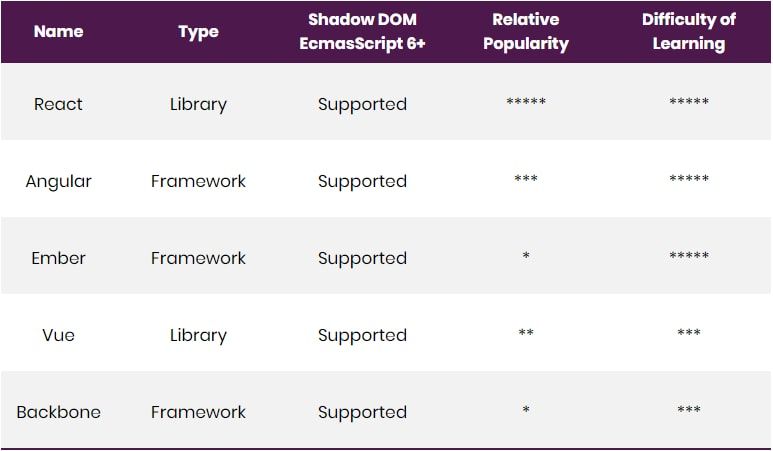
\includegraphics[scale=0.5]{images/comparisonJSFW.jpg}
\caption{Σύγκριση ανάμεσα στα 5 πιο διαδεδομένα \e{frameworks \parencite{javascriptComparison}}}
\label{fig:jsComparison}
\end{figure}
\quadΠαρατηρείται πως τα δύο από αυτά θεωρούνται βιβλιοθήκες. Στην πραγματικότητα όμως η χρησιμότητα και τα χαρακτηριστικά που προσφέρουν μοιάζουν πιο πολύ με ένα σύγχρονο \e{framework}.\par
Η επιλογή ενός για το μελλοντικό έργο , εξαρτάται από τη περιπλοκότητα και τις απαιτήσεις.Για παράδειγμα, το \e{Angular} θεωρείται από τους περισσότερους ιδανικό για τα μεγαλύτερα και πιο περίπλοκα έργα, γιατί τότε θα προσφέρει τα αποτελέσματα που επιθυμούνται.Σε αντίθεση με \e{React, Vue} η ταχύτητα/αποτελεσματικότητα είναι πολύ μειωμένη στα συνηθησμένα μικρά \e{project}.Επίσης απαιτεί απο τους προγραμματιστές περισσότερες γνώσεις και η καμπύλη εκμάθησης (\textlatin{learning-curve}-Σχ.\ref{fig:angular_vue_react_learning_curve}) είναι απότομη.
\begin{figure}[ht]
\centering
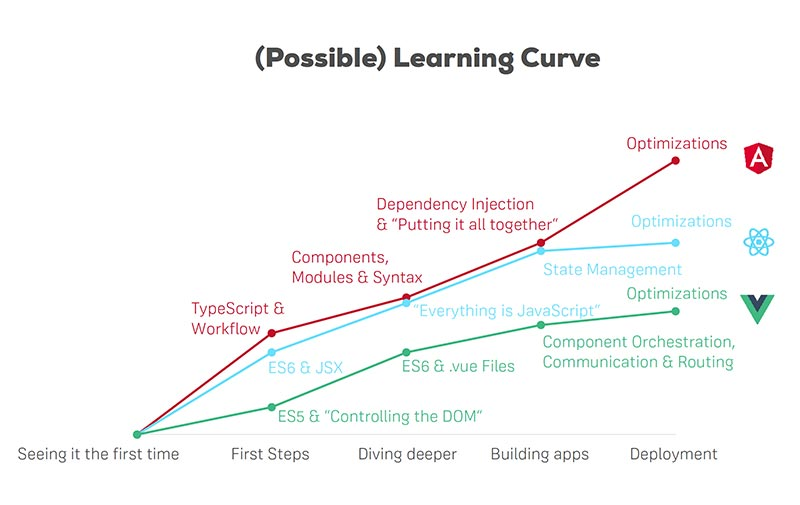
\includegraphics[scale=0.3]{images/angular-react-vue-learning-curve.jpg}
\caption{Κάμπυλη εκμάθησης ανάμεσα σε \e{Angular, React} και \e{Vue frameworks \parencite{angular_vue_react_learning_curve}}}
\label{fig:angular_vue_react_learning_curve}
\end{figure}

\section{\e{RxJS}}
\quadΜια άλλη τεχνολογία που χρησιμοποιήθηκε στην υλοποίηση του έργου της παρούσας πτυχιακής , είναι το \e{RxJS}.Υπό την μορφή μιας βιβλιοθήκης γραμμένη σε \e{JavaScript} με υποστήριξη του \e{TypeScript} , φέρνει την έννοια του αντιδραστικού προγραμματισμού στον ιστό.Αυτό σημαίνει πως η εφαρμογή <<αντιδρά>> στις αλλαγές που συμβαίνουν όπως γεγονότα με επίδραση του χρήστη, λήψη δεδομένων κλπ.

\subsection*{Τι είναι}
\quadΟ αντιδραστικός προγραμματισμός (\e{Reactive Programming}), είναι ένα ασύγχρονο πρότυπο προγραμματισμού που αφορά τις ροές δεδομένων και την διαδόση της αλλαγής.Αυτό σημαίνει ότι είναι δυνατή η εύκολη έκφραση στατικών (π.χ. πίνακες) ή δυναμικών (π.χ.γεγονότα) ροές δεδομένων μέσω της χρησιμοποιούμενης γλώσσας προγραμματισμού, και ότι υπάρχει υποθετική εξάρτηση στο σχετικό μοντέλο εκτέλεσης , πράγμα που διευκολύνει την αυτόματη διάδοση της αλλαγής που σχετίζεται με τη έν λόγο ροή.
Ο ορισμός αυτού του τύπου προγραμματισμού, το δίνει ο γάλλος \e{Gérard Berry} σε μια ερευνητική του έκθεση πάνω σε αυτό το θέμα \e{\parencite{real_time_programming_gerard}}:
\blockquote{Είναι βολικό να διακρίνει κανείς περίπου τρία είδη προγραμμάτων. Τα προγράμματα μετασχηματισμού υπολογίζουν τα αποτελέσματα από ένα δεδομένο σύνολο εισόδων: Τυπικά παραδείγματα είναι οι μεταγλωττιστές ή τα προγράμματα αριθμητικών υπολογισμών.Τα αλληλεπιδραστικά προγράμματα αλληλεπιδρούν με δική τους ρυθμό και ταχύτητα, με τους χρήστες ή άλλα προγράμματα: Από την άποψη του χρήστη, ένα σύστημα \textlatin{Time-Sharing} είναι διαδραστικό. Τα αντιδραστικά προγράμματα διατηρούν επίσης μια συνεχή αλληλεπίδραση με το περιβάλλον τους, αλλά με ταχύτητα που καθορίζεται από το περιβάλλον, όχι από το ίδιο το πρόγραμμα. Τα διαδραστικά προγράμματα λειτουργούν με το δικό τους ρυθμό και ασχολούνται κυρίως με την επικοινωνία, ενώ τα αντιδραστικά προγράμματα λειτουργούν μόνο ως απάντηση στις εξωτερικές απαιτήσεις και συνήθως ασχολούνται με τον ακριβή χειρισμό διακοπών. Τα προγράμματα Πραγματικού Χρόνου είναι συνήθως αντιδραστικά. Ωστόσο, υπάρχουν αντιδραστικά προγράμματα που συνήθως δεν θεωρούνται ότι είναι Πραγματικού Χρόνου, όπως πρωτόκολλα, προγράμματα οδήγησης συστήματος ή χειριστές διεπαφής ανθρώπου-μηχανής.}

\subsection*{Πλεονεκτήματα}
\quadΈνα απο τα πολλά πλεονεκτήματα που προσφέρει ο αντιδραστικός προγραμματισμός στην υλοποίηση ενός έργου, είναι η αποφυγή των \e{Callback}.Παρ'όλο που είναι αρκετά χρήσιμα , τα \textlatin{callbacks} προκαλούν προβλήματα και χάος σε ένα πιο περίπλοκο πρόγραμμα.Για παράδειγμα, αν καλούνται περισσότερες εμφωλευμένες μεθόδους και εμφανίζεται κάποιο σφάλμα , δυσκολεύεται πλέον η συντήρηση και η προσθήκη άλλων χαρακτηριστικών ακόμη πιο πολύ.Το ΑΠ (\e{Reactive-Programming}) λύνει αυτό το θέμα μέσα απο τα \e{Observables, Subjects} κλπ , τα οποία στέλνουν τα δεδομένα , σφάλματα η σήματα τερματισμού εκεί που τα χρειάζεται ο προγραμματιστής.\par
Επίσης, διευκολύνει την δημιουργία πολύπλοκων νημάτων , συγχρονίζοντας παράλληλα την εργασία και τρέχοντας ένα κομμάτι κώδικα όταν όλα τερμάτησαν.Μπορεί κανείς να δημιουργήσει κάποιο νήμα και ύστερα να θέσει ποια συνδρομή να τρέχει πάνω του.Βεβαίως , ένα \e{Observable} για παράδειγμα, μπορεί να τρέχει σε διαφορετικά νήματα ανάλογα με τα φίλτρα που του προσθέτηκαν η την στιγμή που έλαβε τα απαιτούμενα δεδομένα.\par
Αλλά σημαντικά πλεονεκτήματα που αξίζουν να σημειωθούν : 
\begin{itemize}
    \item Προσφέρει το ίδιο <<\e{API}>> για πρόσβαση σε βάση δεδομένων, \e{UI}, υπολογισμό, πρόσβαση στο δίκτυο και ό,τι άλλο χρειαστεί να είναι.
    \item Μόλις καταλάβει κανείς τα βασικά μπορεί να μάθει άλλους χειριστές και φίλτρα όταν τους χρειαστεί, δεν χρειάζεται να ξέρει τα πάντα για να ξεκινήσει.
    \item Οδηγεί σε αναγνώσιμο κώδικα που είναι ευκολότερο να κατανοηθεί, να δοκιμαστεί και να διορθωθεί.
\end{itemize}
Όπως συνήθως , υπάρχουν και κάποια σημεία που μπορούν να θεωρηθούν μειονεκτήματα :
\begin{itemize}
    \item Η απότομη καμπύλη εκμάθησης δεν είναι μόνο λόγω των βιβλιοθηκών, αλλά και λόγω του ότι κάποιος πρέπει να συνηθήσει να σκεφτεί αντιδραστικά
    \item Είναι εύκολο να μην χειριστούν σωστά τις συνδρομές και να εμφανιστούν προβλήματα μνήμης.
\end{itemize}

\subsection*{Εγκατάσταση}
\quad Η εγκατάσταση του \e{RxJS} ,όπως και τα υπόλοιπα, απαιτεί την ύπαρξη του \e{NPM-Node Package Manager} στο σύστημα.Επίσης , το \e{Terminal} πρέπει να βρίσκεται στο φάκελο του έργου στο οποίο προστίθεται η βιβλιοθήκη.Η εντολή που εγκαταστεί την πιο πρόσφατη έκδοση του \e{RxJS} είναι:

\selectlanguage{english}
\begin{lstlisting}[language=command.com]
  $\dollar$ npm install @reactivex/rxjs
\end{lstlisting}
\selectlanguage{greek}

Στην συνέχεια , για να ενσωματωθεί η βιβλιοθήκη στην εργασία,στο αρχείο στο οποίο χρειάζονται, ακολουθούνται τα παρακάτω ανάλογα με τις προτιμήσεις του προγραμματιστή :
\begin{enumerate}
\item Προσθέτωντας όλοκληρη την βιβλιοθήκη (δεν συνιστάται)
\selectlanguage{english}
\begin{lstlisting}[language=Java]
import Rx from 'rxjs/Rx';
\end{lstlisting}
\selectlanguage{greek}
\item Προσθέτωντας μόνο αυτά που χρειάζονται.Για παράδειγμα:
\selectlanguage{english}
\begin{lstlisting}[language=Java]
import { Observable } from 'rxjs/Observable';
import { of } from 'rxjs/observable/of';
import { map } from 'rxjs/operator/map';
\end{lstlisting}
\selectlanguage{greek}
\end{enumerate}

\subsection*{Αλλες επιλογές}
\quadΌσον αφορά το \e{JavaScript}, υπάρχουν αρκετές εναλλακτικές λύσεις για την βιβλιοθήκη που επιλέξαμε:

\selectlanguage{english}
\begin{table}[h!]
\centering
% {\rowcolors{3}{green!80!yellow!50}{green!70!yellow!40}
{\rowcolors{3}{gray!80!black!50}{gray!70!black!40}
\begin{tabular}{ |p{3cm}||p{3cm}|p{3cm}|p{3cm}|  }
 \hline
 \multicolumn{4}{|c|}{\foreignlanguage{greek}{Αντιδραστικές Βιβλιοθήκες} JavaScript} \\
 \hline
 {\foreignlanguage{greek}{Όνομα}} & {\foreignlanguage{greek}{Δημοτικότητα}} & {\foreignlanguage{greek}{Γλώσσα}} & {\foreignlanguage{greek}{Μηναίες Λήψεις}} \\
 \hline\hline
 MobX & 8.6/10 $\uparrow$ & JavaScript & $\sim$840.979\\
 Bacon & 6.9/10 $\downarrow$ & CoffeeScript & $\sim$35,437\\
 Highland & 4.9/10 $\uparrow$ & JavaScript & $\sim$60,614\\
 MostJS & 4.6/10 $\uparrow$ & JavaScript & $\sim$63,340\\
 \hline\hline
 \rowcolor{red!80!black!50}
 RxJS & 9.4/10 $\uparrow$ & JavaScript & $\sim$3,889,703\\
 \hline
\end{tabular}}
\caption{\foreignlanguage{greek}{Σύγκριση ανάμεσα στις πιο δημοφιλές βιβλιοθήκες\foreignlanguage{english}{\parencite{awesomejs_reactive}}}}
\label{table:reactive_programming_libraries_comparison}
\end{table}
\selectlanguage{greek}

Από τον πίνακα \ref{table:reactive_programming_libraries_comparison} , μπορεί κανείς να συμπεράνει πως το \e{RxJS} έχει την μεγαλύτερη κοινότητα προγραμματιστών σύμφωνα με τις μηναίες λήψεις και δημοτικότητα.Όπως είναι γνωστόν , αυτό το χαρακτηριστικό αποδεικνύεται κρίσιμο είδικα όταν η έννοια του αντιδραστικού προγραμματισμού δέν είναι εύκολη κατανοητή από όλους.

\section{\e{Google Material Design}}
\quadΤο \e{Material Design} της \textlatin{Google} είναι μια έννοια , ένα ενοποιημένο σύστημα σχεδιασμού, που σχεδιάστηκε για να είναι διαθέσιμο σε όλες τις σημερινές πλατφόρμες.Όλος ο σχεδιασμός πρέπει να φαίνεται και να αισθανθεί ίδιο όπου και αν συμπεριλαμβάνεται.

Υπάρχουν τρεις βασικές αρχές που κατασκευάζουν αυτήν την έννοια, τα οποία αποτελούν την βάση του \e{Material Design}:

\begin{itemize}
    \item Είναι μια μεταφορική έννοια.Η ανάπτυξη του συστήματος εμπνεύστηκε από τη μελέτη των απτικών στοιχείων που συναντιούνται στην καθημερινότητα, δηλαδή του χαρτιού και μελανιού. 
    \item Έντονη, γραφική και σκόπιμη. Η τυπογραφία, τα πλέγματα, ο χώρος, η κλίμακα, το χρώμα και η χρήση των εικόνων που χρησιμοποιούνται στη βασική σχεδίαση, καθιστούν το περιεχόμενο του \e{Material} καλύτερο.
    \item Η κίνηση παρέχει νόημα - αυτό είναι ένα από τα πιο γνωστά πράγματα. Στο \e{Material Design}, θα βρείτε ουσιαστικές και κατάλληλες κινήσεις, λεπτές και ξεκάθαρες ανατροφοδοτήσεις, και αποτελεσματική και συνεπή μετάβαση.
\end{itemize}

Το σημαντικό πράγμα που πρέπει να καταλάβει κανείς σχετικά με το \e{Material Design} είναι ότι θεωρείται μια γλώσσα σχεδιασμού, μια έννοια, ένα ενοποιημένο σύστημα σχεδιασμού. Δεν είναι ένα πακέτο \e{UI} ή μια συλλογή στοιχείων , αλλά ένας νέος τρόπος να μιλάμε και να κοιτάμε το γραφικό περιβάλλον.

\subsection*{\e{Angular Material Design}}
\quadΟ στόχος του είναι να προσφέρει ένα σύνολο υψηλής ποιότητας στοιχείων \e{UI} που έχουν σχεδιαστεί για το \e{Angular} υποστηρίζοντας το υπερσύνολο του \textlatin{JavaScript}, το γνωστό \e{TypeScript}.Αυτό το σύνολο στοιχείων , ακολουθεί την έννοια του \e{Material Design} και το σύστημα σχεδιασμού, που περιγράφεται στο προηγούμενο υποκεφάλαιο.\par
Συμπεριλαμβάνει αρκετά έτοιμα στοιχεία , τα οποία εισάγονται στο έργο πολύ εύκολα.Χρησιμοποιώντας τα , ένας προγραμματιστής μπορεί να συγκεντρωθεί παραπάνω στην λειτουργικότητα του έργου παρά στην σχεδίαση , όπου συνήθως χρειάζεται πολύς χρόνος.\par

\subsection*{Εγκατάσταση}
\quadΗ εγκατάσταση του σε περιβάλλον \e{Angular} επιτυγχάνεται μέσα σε έξι βήματα:
\begin{enumerate}[label=\textbf{\arabic*}]
    \item 
\selectlanguage{english}
\begin{lstlisting}[language=command.com]
  $\dollar$ npm install --save @angular/material @angular/cdk
\end{lstlisting}
\selectlanguage{greek}
    \item Το \e{Material} χρησιμοποιεί \e{WebAnimations API},το οποίο δεν έχει ακόμη υποστήριξη σε όλα τα προγράμματα περιήγησης.Η εντολή \e{bash} είναι ως ακόλουθη:   
\selectlanguage{english}
\begin{lstlisting}[language=command.com]
  $\dollar$ npm install --save @angular/animations
\end{lstlisting}
\selectlanguage{greek}
Υπάρχουν δύο τρόπους εισαγωγής αυτού του \e{module}:
    \begin{itemize}
        \item Να προστεθεί το \e{polyfill} των \e{WebAnimation} και να εισαχθεί στο \e{Module} που χρειάζεται, το \e{Angular Animation}:
\selectlanguage{english}
\begin{lstlisting}[language=Java]
    import {BrowserAnimationsModule} from 
        '@angular/platform-browser/animations';

    @NgModule({
      ...
      imports: [BrowserAnimationsModule],
      ...
    })
    export class AppModule { }
\end{lstlisting}
\selectlanguage{greek}
    \item  Να χρησιμοποιήσει το \e{module, NoopAnimationsModule} όπως παρακάτω  
\selectlanguage{english}
\begin{lstlisting}[language=Java]
    import {NoopAnimationsModule} from 
        '@angular/platform-browser/animations';

    @NgModule({
      ...
      imports: [NoopAnimationsModule],
      ...
    })
    export class AppModule { }
\end{lstlisting}
\selectlanguage{greek}
    \end{itemize}
    \item Σε αυτό το βήμα, εισάγονται τα στοιχεία/κομμάτια που θα χρησιμοποιηθούν.
    Βεβαίως, μπορούν να προστεθούν και αργότερα παραπάνω, ανάλογα με τις απαιτήσεις.
    Για παράδειγμα, σύμφωνα με τα παρακάτω θα εισαχθούν δύο στοιχεία μόνο, κουμπιά και \e{checkbox}.
\selectlanguage{english}
\begin{lstlisting}[language=Java]
   import {MatButtonModule, MatCheckboxModule} 
        from '@angular/material';

    @NgModule({
      ...
      imports: [MatButtonModule, MatCheckboxModule],
      ...
    })
    export class AppModule { }
\end{lstlisting}
\selectlanguage{greek}
Υπάρχει όμως ένας καλύτερος τρόπος για την εισαγωγή.Προτείνεται να δημιουργηθεί ένα ξεχωριστό \e{module} που να περιέχει όλα τα στοιχεία που θα χρησιμοποιηθούν, και ύστερα αυτό να προστεθεί στο γενικό.Για παράδειγμα:
\selectlanguage{english}
\begin{lstlisting}[language=Java]
   import {MatButtonModule, MatCheckboxModule} 
    from '@angular/material';

    @NgModule({
      imports: [MatButtonModule, MatCheckboxModule],
      exports: [MatButtonModule, MatCheckboxModule],
    })
    export class MyOwnCustomMaterialModule { }
\end{lstlisting}
\selectlanguage{greek}
Όποιο τρόπο και να επιλεχθεί, η εισαγωγή πρέπει να γίνει μετά του \e{Browser Module} του \e{Angular}
    \item Στην συνέχεια , για να εμφανίζονται τα στοιχεία , πρέπει να εισαχθεί στο γενικό αρχείο \e{CSS}, το σχεδιαστικό θέμα του \e{Material}:
\selectlanguage{english}
\begin{lstlisting}[language=JAVA]
@import "~@angular/material/
prebuilt-themes/indigo-pink.css";
\end{lstlisting}
\selectlanguage{greek}
Σημειώνεται, πώς υπάρχουν τέσσερα σχεδιαστικά θέματα αλλά μπορεί κανείς να δημιουργεί μιά ιδιωτική.
    \item Επιπλέον , όπως αναφέρεται και στους ορισμούς, οι κινήσεις θεωρούνται ένα πολύ σημαντικό θέμα.Για να υποστηρηχθούν αυτά , θά πρέπει να είναι εγκατεστημένο και το \e{HammerJS}:
\selectlanguage{english}
\begin{lstlisting}[language=command.com]
   $\dollar$ npm install --save hammerjs
\end{lstlisting}
\selectlanguage{greek}
Ύστερα η εισαγωγή στο αρχικό \e{component} της εφαρμογής:
\selectlanguage{english}
\begin{lstlisting}[language=JAVA]
   import 'hammerjs';
\end{lstlisting}
\selectlanguage{greek}
    \item Αυτό το βήμα είναι προαιρετηκό, αλλά συνιστάται, αφού προσθέτει μια αναφορά προς τα εικονίδια τύπου \e{Material}:
\selectlanguage{english}
\begin{lstlisting}[language=JAVA]
<link href="https://fonts.googleapis.com/icon?
family=Material+Icons" rel="stylesheet">
\end{lstlisting}
\selectlanguage{greek}
\end{enumerate}

\quad Αφού ολοκληρωθούν τα πρώτα πέντε τουλάχιστον παραπάνω βήματα, μπορεί κανείς να χρησιμοποιήσει τα στοιχεία του \e{Angular Material Design} όπως στο παράδειγμα:
\selectlanguage{english}
\begin{lstlisting}[language=JAVA]
<mat-tab-group>
  <mat-tab label="Tab 1">Content 1</mat-tab>
  <mat-tab label="Tab 2">Content 2</mat-tab>
</mat-tab-group>
\end{lstlisting}
\selectlanguage{greek}
Αυτά εισάγουν στον χώρο μια συλλογή των δυό καρτέλων με ετικέτες <<\e{Tab 1}>> και <<\e{Tab 2}>>.Τα χρώματα και τα εφέ στις αλλαγές καρτέλας είναι έτοιμα, όπως και ήταν αναμενόμενο.

\subsection*{Αλλες επιλογές}
% PrimeNG , WEBMATERIAL
\quadΥπάρχουν και άλλες βιβλιοθήκες διαθέσιμες για την κατασκεύη των εφαρμογών \e{web} σε περιβάλλον \e{Angular}, όπως \e{PrimeNG, WMD - Web Material Design} ή \e{Bootstrap}.Τα τελευταία δύο είναι \e{Cross-Platform}, δηλαδή έχουν την δυνατότητα να εισάγονται σε οποιοδήποτε περιβάλλον.\newline
\quadΤο \e{Bootstrap} είναι μια συλλογή εργαλείων ανοιχτού κώδικα που περιέχει \e{HTML} και \e{CSS} για τις μορφές τυπογραφίας, κουμπιά πλοήγησης και άλλων στοιχείων του περιβάλλοντος, καθώς και προαιρετικές επεκτάσεις \e{JavaScript}.
Τo \e{Web Material Design} ακολουθεί την ίδια έννοια οπως το \e{Material} που χρησιμοποιήθηκε για αυτήν την εργασία, με την διαφορά ότι διαθέτει τα στοιχεία με τον ίδιο τρόπο του \e{Bootstrap}, γι'αυτό και θεωρείται \e{Cross-Platform}.
Η τρίτη βιβλιοθήκη που αναφέρθηκε, \e{PrimeNG}, είναι αποκλειστικά για \e{Angular}, εφόσον τα στοιχεία που περιέχει διαθέτονται με την μορφή \e{Components, Derivative}.Το μεγαλύτερο πλεονέκτημα που έχει σε σχέση με \e{Angular Material Design} είναι το πλήθος των στοιχείων , δηλαδή πάνω απο εβδομήντα σε αντίθεση με τα τριάνταδύο που προσφέρει μέχρι στιγμής το \e{Material 2}.

\section{\e{WebStorm}}
\quadΟι προγραμματιστές για να διευκολύνουν την δουλειά τους και την γραφή κώδικα, χρησιμοποιούν σύχρονα \e{IDE}.Ένα \e{IDE} είναι ένα ολοκληρωμένο περιβάλλον ανάπτυξης \e{(integrated development environment, IDE)}, μία σουίτα λογισμικού που βοηθάει στην ανάπτυξη εφαρμογών. Συνήθως ένα \e{IDE} περιλαμβάνει κάποιον επεξεργαστή πηγαίου κώδικα, έναν μεταγλωττιστή, εργαλεία αυτόματης παραγωγής κώδικα, αποσφαλματωτή, συνδέτη, σύστημα ελέγχου εκδόσεων και εργαλεία κατασκευής γραφικών διασυνδέσεων χρήστη για τις υπό ανάπτυξη εφαρμογές.Βεβαίως η ανάπτυξη των λογισμικών δεν εξαρτάται από αυτό, εφόσον κάποιος θα μπορούσε να γράψει κώδικα σε ένα απλό επεξεργαστή κειμένου. Τα \e{IDE} προτείνονται στους και προτιμούνται από τους περισσότερους προγραμματιστές, ειδικά από αρχάριους.Για να φθάσει κανείς να χρησιμοποιεί μόνο ένα απλό επεξεργαστή κειμένου στην ανάπτυξη και να καταφέρει μέγιστη αποτελεσματικότητα, θα πρέπει να βρίσκεται σε έναν πολύ υψηλό επίπεδο γνώσεων.\newline

\subsection*{Τι είναι}
\quadΣτην παρούσα πτυχιακή εργασία, η ανάπτυξη λογισμικού ολοκληρώθηκε στο περιβάλλον του \e{WebStorm}, προιόν της εταιρίας \e{JetBrains}.Η άδεια ήταν δωρεάν για ένα χρόνο, λόγω της στήριξης των φοιτητών, αλλιώς ένας ιδιώτης θα έπρεπε να επιλέξει ανάμεσα στην μηναία συνδρομή των έξι ευρώ η την ετήσια των εξήντα ευρώ.\newline
\quadΤα πιο προφανές χαρακτηριστικά σύμφωνα με την ιστοσελίδα του προιόντος (\e{\cite{webstorm}}):
\begin{itemize}
    \item Έξυπνη βοήθεια στην ανάπτυξη:
        \begin{itemize}
            \item Υποστήριξη σύγχρονων \e{framework}
            \item Ολοκλήρωση κώδικα και εντοπισμός σφαλμάτων κατά την πληκτρολόγηση
            \item Πλοήγηση και αναζήτηση, ματάβαση σε μεθόδους κλπ
        \end{itemize}
    \item Επεξεργασία σφαλμάτων, εντοπισμός και έλεγχος
        \begin{itemize}
            \item \e{Debugging}
            \item \e{Testing}
            \item Εξερεύνηση του τρόπου με το οποίο τα αρχεία συνδέονται
        \end{itemize}
    \item Εύκολη ενσωμάτωση εργαλείων
        \begin{itemize}
            \item Εργαλεία ανάπτυξης (π.χ \e{npm})
            \item Εργαλεία ποιότητας κώδικας
            \item Πρότυπα εργασίας
        \end{itemize}
    \item Άλλα χρήσημα χαρακτηριστικά
        \begin{itemize}
            \item \e{Version Control System} (π.χ. \e{GitHub})
            \item Τοπικό ιστορικό ενός αρχείο η εργασίας
            \item Προσαρμογή στις προτιμήσεις καθενός
        \end{itemize}
\end{itemize}

\subsection*{Πλεονεκτήματα}
\quadΟι συντομεύσεις είναι ίσως απο τα πιό πολύτιμα χαρακτηριστικά ενός περιβάλλον ανάπτυξης.Χάρη σε αυτά ένας προγραμματιστής βελτιώνει την αποτελεσματικότητα του με 10 έως και 50 \%.
\begin{itemize}
    \item Έλεγχος σφαλμάτων - Έλεγχος ορθής ορθογραφίας για τον κώδικα. Απολύτως απαραίτητο.
    \item Πλοήγηση - \keys{\e{\ctrl}} + κλίκ σε μια συνάρτηση, μεταβλητή η τύπος για μετάβαση στον ορισμό.
    \item Ολοκλήρωση κώδικα - \keys{\e{\ctrl}} + \keys{\e{\space}} Συμπληρώνει το όνομα κλάσης ή μεθόδου που χρειάζεται. Αυτό επιταχύνει την ανάπτυξη σοβαρά και ακόμα βοηθάει να εντοπίσει κανείς σφάλματα προτού συμβούν όταν κάτι που χρειάζεται δεν είναι προσβάσιμο από το περιβάλλον στο οποίο βρίσκετε.
    \item Συμπλήρωση/Δημιουργία κώδικα - Δημιουργεί \e{getters} και \e{setters}, εφαρμόζει μεθόδους από μια διεπαφή με μερικά κλικ.
    \item Πολύ καλό χρωματισμό κώδικα - \e{WebStorm} όχι μόνο χρωματίζει την λέξη-κλειδί, συμβολοσειρά,μεταβλητή, αλλά και μεταβλητές κλάσης, τοπικές μεταβλητές, παραμέτρους.
    \item Αυτόματη διόρθωση - Η λανθασμένη μετονομασία συμβαίνει πολλές φορές. Το \e{WebStorm} είναι πολύ καλό για τη μετονομασία ακόμη και των \e{setters,getters} ή των \e{strings}.
    \item Η ενσωμάτωση συστήματος ελέγχου έκδοσης (\e{VCS}) - Τα \e{merge} σφάλματα αναπαριστάνονται μέσα στο περιβάλλον , διευκολύνοντας κατα πολύ αυτό το βήμα.
    \item Εισαγωγή βιβλιοθήκων - Μπορεί κανείς εύκολα να μεταβεί στον κώδικα της βιβλιοθήκης για αναφορά, εντοπισμό σφαλμάτων κλπ.
   \item Έξυπνη πληκτρολόγηση - Αυτόματη συμπλήρωση τελικών στηριγμάτων, παρενθέσεις, εισαγωγικά κλπ.
   \item \e{Debugging} - Ίσως το πράγμα που οι περισσότεροι προγραμματιστές λατρευόυν.Χωρίς αυτό η ανάπτυξη λογισμικού θα ήταν πολύ δυσκολότερη.
\end{itemize}

\subsection*{Αλλες επιλογές}
\quadΗ κύρια εναλλακτική λύση για το \e{WebStorm} είναι το δωρεάν \e{Visual Studio Code} της \e{Microsoft}.\newline
Έχοντας γράψει κώδικα και στις δύο σουίτες, καταλήξαμε στο ίδιο συμπέρασμα ομαδικά, πως το \e{WebStorm} είναι προς το παρόν πιο <<ώριμο>> σε αρκετά θέματα κλειδί.

\chapter{\e{Project Management} Εργαλεία}
Στο κεφάλαιο αυτό αρχικά αναφέρονται κάποιες εφαρμογές που χρησιμοποιούνται παγκοσμίως σήμερα, για την διαχείριση έργων.Στην συνέχεια, περιγράφεται σε γενικές γραμμές η εφαρμογή \e{iPM}, η αρχιτεκτονική της και ύστερα οι λειτουργίες της ως προς των κώδικα.

\section{Έρευνα αγοράς}

\subsection{\e{Asana}}
\quad Το \e{Asana} είναι ίσως η πιο γνωστή εφαρμογή που έχει σχεδιαστεί για να βοηθήσει τις ομάδες να παρακολουθούν τα έργα τους.\\
\pSpace Κάθε ομάδα μπορεί να δημιουργήσει ένα χώρο εργασίας. Οι χώροι εργασίας περιέχουν έργα και τα έργα περιέχουν εργασίες. Σε κάθε εργασία, οι χρήστες μπορούν να προσθέτουν σημειώσεις, σχόλια, συνημμένα και ετικέτες. Οι χρήστες μπορούν να ακολουθήσουν τα έργα και τις εργασίες και, όταν αλλάξει η κατάσταση ενός έργου ή μιας εργασίας, οι ακόλουθοι λαμβάνουν ενημερώσεις σχετικά με τις αλλαγές στα εισερχόμενά τους. \e{\parencite{asana_wiki}} Αυτό βοηθάει την παρακολούθηση των εργασιών από την αρχή μέχρι το τέλος, την ανάθεση υποεργασιών σε μέλη της ομάδας και τον καθορισμό προθεσμιών για να διασφαλιστεί ότι τα έργα θα γίνουν εγκαίρως. Έτσι ομάδες εργάζονται πιο παραγωγικά και αποτελεσματικά. \e{\parencite{asana_task}}\\
\pSpace Ένα άλλο πολύ σημαντικό χαρακτηριστικό αυτής της εφαρμογής είναι το ότι προσφέρει την δυνατότητα να χρησημοποιηθεί το \e{API} τους απο τρίτους. Επομένως, εφαρμογές όπως \e{Dropbox, Evernote, GoogleDrive, Instagantt, Jira} και άλλα, μπορούν να συνδεθούν με τον λογαριασμό \e{Asana}, ετσι ώστε να μεγαλώσει την παραγωγικότητα του χρήστη.

\subsection{\e{Trello}}
\pSpace Άλλη μια διαδικτυακή εφαρμογή που αξίζει να σημειωθεί είναι το \e{Trello}, τωρα υπό το όνομα \e{Attlassian}. Το απλό \e{design} και η δυνατότητα \e{Agile} κέρδισε πελάτες πολύ εύκολα.\\
\pSpace Επίσης η ικανότητα να συνδέσει κανείς το \e{dashboard} με υπηρεσίες όπως \e{Slack} και \e{GitHub} φέρνει ένα σημαντικό πλεονέκτημα σε σχέση με άλλες εφαρμογές. 

\section{\e{iPM} - Γενική Περιγραφή}
\pSpace'Οπως προαναφέρθηκε, ο σκοπός της πτυχιακής είναι η ανάπτυξη μιας διαδικτυακής εφαρμογής για την διαχείριση έργων, το οποίο ονομάστηκε \e{iPM}.\\
\pSpace Ο χρήστης δημιουργεί έναν λογαριασμό για να έχει πρόσβαση στην εφαρμογή, όπου μπορεί να δημιουργήσει καινούργια έργα ή να διαχειρίσει ήδη υπάρχοντα αν είναι μέλος η διαχειριστής αυτόν. Για να συμβάλλει σε κάποιο άλλο έργο, θα πρέπει να τον καλέσει κάποιο μέλος εκείνου του εργου, και αφού δεχτεί θα μπορεί να δεί λεπτομέριες, να του ανατεθούν εργασίες, η να πάρει μέρος στις συζητήσεις που αφορούν το συγκεκριμένο έργο.\\
\pSpace Ο χρήστης μπορεί να παρακολουθεί την πρόοδο του έργου μέσα απο τα διαγραμμάτα στον χώρο εργασίας έργου και απο τα διαγράμματα Γκαντ. Επίσης κάθε μέλος ενημερώνεται άμεσα για κάθε ένεργεια που τον αφορά προσωπικά.

\subsection*{\e{Use Cases}}
\pSpace Στο παρακάτω \e{UML} διάγραμμα φαίνονται τα βασικά \e{Use Cases} της εφαρμογής.
\begin{figure}[ht]
\centering
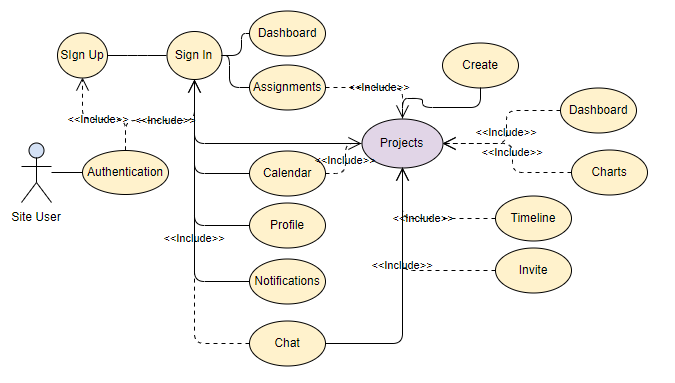
\includegraphics[scale=1]{images/usecase.jpg}
\caption{\e{UML Use Cases}}
\label{fig:use_cases}
\end{figure}
\pagebreak

\subsection*{Χάρτης Εφαρμογής - \e{Site map}}
\dirtree{%
.1 \e{Homepage}.
.1 \e{Auth}.
.2 \e{Sign Up}.
.3 \e{Sign In}.
.1 \e{App}.
.2 \e{Dashboard}.
.2 \e{My Projects}.
.3 \e{Project}.
.4 \e{Dashboard}.
.4 \e{Assignments}.
.5 \e{Classic}.
.5 \e{Agile}.
.4 \e{Gantt}.
.4 \e{Team}.
.4 \e{Timeline}.
.4 \e{Chat}.
.4 \e{Settings}.
.2 \e{My Tasks}.
.2 \e{My Issues}.
.2 \e{Calendar}.
.2 \e{Chat}.
.2 \e{Profile}.
.2 \e{Invites}.
}

\subsection*{Υποθέσεις και εξαρτήσεις}
\pSpace Δεδομένου ότι είναι μια διαδικτυακή εφαρμογή, το τελικό προιόν θα είναι προσβάσιμο μέσω ίντερνετ απο περιηγητή ιστού (\e{Web Browser}) τελευταίας έκδοσης. Δέν υποστηρίζεται δυνατότητα \e{offline}.

\section{\e{Specific Requirements}}
\subsection*{\e{User Stories}}
\pSpace Όπως προκύπτει και απο σχ. \ref{fig:use_cases} τα \e{User Stories} πηγαίνουν ως εξής:
\begin{itemize}
	\item Ο χρήστης μπορεί να δημιουργήσει έναν λογαριασμό παρέχοντας μια ηλεκτρονική διεύθυνση (\e{email}) και κωδικό.
	\item Η σύνδεση στην εφαρμογή επιτυγχάνεται με τα δεδομένα που προμηθεύτηκαν στο στάδιο εγγραφής.
	\item Στον χώρο εργασίας χρήστη φαίνονται τα \e{assignments} που χρειάζονται την προσοχή όπως και συντομεύσεις για τα έργα στα οποία είναι μέλος.
	\item Επίσης ο χρήστης μπορεί να δεί τις εργασίες που του αναθέτηκαν ανά τύπο (\e{Task/Issue}) και να χρησιμοποιήσει την συντόμευσή της.
	\item Ακόμη, έχει την δυνατότητα να αλλάξει τις πληροφορίες μέσα απο το προφίλ
	\item Στο ημερολόγιο φαίνονται όλα τα γεγονότα, είτε προσωπικά είτε κάποιου έργου.
	\item Οι ειδοποιήσεις έχουν πρόσβαση από παντού, και καλύπτουν τα γεγονότα που χρειάζονται προσοχή.
	\item Επιπλεόν στο \e{Chat} υπάρχουν όλες οι συζητήσεις έργων, και ο χρήστης μπορεί να συμβάλλει σε αυτά σε πραγματικό χρόνο.
	\item Ο χρήστης φυσικά μπορεί να δημιουργήσει και να διαχειριστεί έργα.
	\item Έχει την δυνατότητα να καλέσει χρήστες που έχουν λογαριασμό στην εφαρμογή, σε κάποιο έργο.
	\item Επιπροσθέτως, μπορεί να αναθέτει εργασίες στα μέλοι έργου.
	\item Για την καλύτερη και ομαλότερη εμπειρία, ο χρήστης μπορεί να φιλτράρει τις εργασίες με βάση όνομα, μέλος, κατάσταση η/και τύπο.
	\item Ο διαχειριστής μπορεί να δεί και να αλλάξει τις πληροφορίες και τις ρυθμίσεις του έργου.
	\item Ο χρήστης μπορεί να παρακολουθεί την πρόοδο με οπτικό τρόπο, απο τα διαγράμματα. Επίσης μπορεί να αποθηκεύσει στην συσκεύη κάποιο διάγραμμα για άλλη χρήση.
\end{itemize}

\subsection*{\e{System Requirements}}
\pSpace Η εφαρμογή ανήκει στην γενιά \e{Web 2.0} εφόσον είναι \e{Centralized} τύπου. Οπότε, για τους σκοπούς αυτής της πτυχιακής εργασίας, το δωρεάν \e{domain} της \e{Heroku} και την επίσης δωρεάν έκδοση της \e{mLab} καλύπτουν πλήρως τις ανάγκες της εν λόγω εφαρμογής.
\pagebreak

\section{Αρχιτεκτονική}

\subsection*{Δομή του έργου}
\pSpace Το πρότζεκτ έχει την ακόλουθη δομή:\\
\dirtree{%
.1 \e{iPM}.
.2 \e{src}.
.3 \e{client}.
.3 \e{config}.
.3 \e{e2e}.
.3 \e{server}.
.3 \e{main.ts}.
.2 \e{.angular-cli.json}.
.2 \e{.editorcofig}.
.2 \e{package.json}.
.2 \e{tsconfig.json}.
.2 \e{tslint.json}.
.2 \e{typings.json}.
.2 \e{webpack.config.js}.
.2 \e{.gitignore}.
}

\pSpace Ο φάκελος \e{src} περιλαμβάνει όλη την εφαρμογή, \e{front-end} και \e{back-end}, ενώ τα υπόλοιπα αρχεία προμηθεύουν τις ρυθμίσεις και τα απαραίτητα για την εγκατάστση της εφαρμογής.\\
\pSpace Συγκεκριμένα:
\begin{itemize}
	\item Στο \e{.angular-cli.json} προσθέτονται οι εφαρμογές που θα τρέξουν, και για την κάθε μια ρυθμίζονται που θα αποθηκεύτει το έτοιμο πακέτο, ποιο έιναι τα \e{root} όσον αφορά την \e{main, index, polyfills, test} και καθολικά στύλ. Δηλαδή εδώ υπάρχουν οι αναφορές για οτι αφορά τις εφαρμογές \e{Angular}.
	\item \e{.editorconfig} κρατάει τις ρυθμίσεις για το \e{coding-style} που χρησιμοποιείται. Αυτό σημαίνει πώς αν αυτό το πρότζεκτ θα ανοιχτεί σε ενα διαφορετικό \e{IDE} από αυτό στο οποίο δημιουργήθηκε, ο κώδικας θα φανεί όπως είναι αναμενόμενο, με τα σωστά κενά κλπ.
	\item Το αρχείο \e{package.json} αποθηκεύει τα \e{script} που κατασκεύαζουν η τρέχουν την εφαρμογή, αλλά και τις εξαρτήσεις.
	\item Στο \e{tsconfig.json} βρίσκονται οι απαραίτητες ρυθμίσεις για το \e{TypeScript}, εφόσον η εν λόγω εφαρμογή γράφτηκε χρησιμοποιώντας αυτό το \e{super-script} της \e{JavaScript}.
	\item Δεδομένου ότι ασχολήθηκαν δύο άτομα στην ανάπτυηξη της εφαρμογής, για μια ομαλότερη εμπειρία, χρησιμοποίηθηκε το \e{TypeScript Lint}, έτσι ώστε να κυριαρχεί ένα \e{Coding Style}. 
	\item Οι ρυθμίσεις του \e{module builder (Webpack)} βρίσκονται στο αντίστοιχο αρχείο \e{.js}.
	\item Τελευταίο, το αρχείο \e{.gitignore} χρειάστηκε τόσο για το \e{GitHub} αλλά και για το \e{Heroku}, όπου ανεβάσαμε την εφαρμογή. Με αυτόν τον τρόπο ανεβαίνουν μόνο τα απαραίτητα αρχεία.
\end{itemize}
\pSpace Στρέφοντας την προσοχή πίσω στον φάκελο \e{src}, παρατηρούνται τα εξής:
\dirtree{%
.1 \e{src}.
.2 \e{client}.
.2 \e{config}.
.2 \e{e2e}.
.2 \e{server}.
.2 \e{main.ts}.
}
\pSpace Ο φάκελος \e{client} περιλαμβάνει το \e{front-end}, στο \e{e2e} βρίσκονται τα \e{test} ενώ τα υπόλοιπα αποτελούν τον \e{server}.

\pSpace Το αρχείο \e{main.ts} είναι υπεύθυνο για να ξεκινήσει ο \e{server}, η βάση δεδομένων και το \e{Socket.io}, όπως και την διαχείρηση των διαδρομών. Εφόσον η εφαρμογή είναι \e{One-Page Application} οποιαδήποτε διαδρομή εκτός του \e{/api...} θα διαχιρίζεται απο το \e{Angular}.\\
\pSpace Παρακάτω φαίνονται τα περιεχόμενα του φακέλου \e{server}: 
\dirtree{%
.1 \e{server}.
.2 \e{database}.
.3 \e{dbClient.ts}.
.3 \e{utils.ts}.
.2 \e{routes}.
.3 \e{assignments}.
.3 \e{auth.ts}.
.3 \e{calendar.ts}.
.3 \e{chat.ts}.
.3 \e{invite.ts}.
.3 \e{notifications.ts}.
.3 \e{project.ts}.
.3 \e{settings.ts}.
.3 \e{timeline.ts}.
.3 \e{user.ts}.
.2 \e{controller.ts}.
.2 \e{socket.ts}.
.2 \e{utils.ts}.
}

\pSpace Συνεχίζοντας στο κομμάτι του \e{client}, παρατηρείται η παρακάτω δομή:
\dirtree{%
.1 \e{client}.
.2 \e{app}.
.2 \e{assets}.
.2 \e{index.html}.
.2 \e{karma.conf.js}.
.2 \e{main.server.ts}.
.2 \e{main.ts}.
.2 \e{polyfills.ts}.
.2 \e{test.ts}.
.2 \e{tsconfig.app.json}.
.2 \e{tsconfig.server.json}.
.2 \e{ts.config.spec.json}.
.2 \e{typings.d.ts}.
}
\pSpace Στον φάκελο \e{app} βρίσκονται όλα τα \e{component}, ενώ στο \e{assets} περιλαμβάνονται τα καθολικά \e{scss} και εικόνες οι οποίες χρησιμοποιήθηκαν στην εφαρμογή.\\
\pSpace Το \e{index.html} είναι η σελίδα στην οποία θα προσθετεί το δυναμικό περιεχόμενο. Περιέχει τα απαραίτητα \e{metadata}, διευθύνσεις για εικονίδια, διαγράμματα και το \e{tag "app-root"} που αφορά το περιεχόμενο της εφαρμογής. Στα υπόλοιπα αρχεία βρίσκονται οι ρυθμίσεις του \e{Angular}, \e{test} και του \e{Typescript}.
\selectlanguage{greek}
\section{Αναλυτική περιγραφή της εφαρμογής}
\pSpace Σε αυτό το κεφάλαιο, περιγράφονται αναλυτικά τα σημαντικά κομμάτια της εφαρμογής. Ξεκινώντας με τον \e{server} και το \e{api}, στην συνέχεια θα αναφέρονται τα \e{component} του \e{front-end}, η δομή και η λογική τους, και στο τέλος η βάση δεδομένων.

\subsection{\e{Server}}
\pSpace Ο \e{server} είναι γραμμένος σε \e{TypeScript} όπως και το υπόλοιπο της εφαρμογής και τρέχει πάνω σε πρωτόκολλο \e{HTTP} και περιβάλλον \e{NodeJS}. Επίσης προστέθηκε και ένας \e{server Socket.io} ο οποίος τρέχει παράλληλα με τον αρχικό, στο ίδιο \e{domain} και θύρα.\\
\pSpace Το \e{ExpressJS framework} βοηθάει στην καλύτερη οργάνωση του διακομιστή, αλλά ταυτόχρονα κάνει όλη την εμπειρία να κυλάει πιο ομαλά. Με την βοήθειά του, οι ρυθμίσεις για τον τύπο δεδομένων που στέλνονται και δέχονται, διαδρομές και μεθόδους επαλήθευσης πριν την πρόσβαση σε ενα συγκεκριμένο \e{endpoint}, επιτυχάνονται με λιγότερο κώδικα.\\
\pSpace Για την καλύτερη οργάνωση, δημιουργήθηκε μια κλάση \e{IOServer} η οποία εξυπηρετεί μόνο το \e{Socket.io}. Αυτή η κλάση περιλαμβάνει ιδιωτικές μεταβλητές οι οποίες αποθηκεύουν τα \e{id} των τρέχων \e{socket}/χρηστών, δωματιών (ενα δωμάτιο ανά έργο) αλλά και μεθόδους για αποστολή δεδομένων σε συγκεκριμένα δωμάτια. Ο \e{constructor} της παίρνει ως παράμετρο το αρχικό \e{server}, για να σιγουρεύτει ότι ξεκινάει όντως παράλληλα με τον πρώτο και στην συνέχεια περιμένει/<<ακούει>> για συγκεκριμένα μηνύματα που ανταλάσσονται στο \e{IOServer}. Για παράδειγμα, την στιγμή που ένας χρήστης συνδεέται στην εφαρμογή, στέλνεται αυτόματα ένα μήνυμα στο \e{io} διακομιστή μαζί με το \e{token} του χρήστη. Επαληθεύεται το \e{token} και ο χρήστης προστίθεται στα δωμάτια ανήκει. Έτσι του δίνεται η δυνατότητα να λαμβάνει σημαντικά γεγονότα σε πραγματικό χρόνο. Παρακάτω παρουσιάζονται δύο παραδείγματα που καλύπτουν την αποστολή και την λήψη δεδομένων πάνω σε \e{Socket.io}.\\
\pSpace Για την άποστολή δεδομένων υπάρχουν δύο τρόπους:
\begin{itemize}
	\item Στην περίπτωση που στέλνει στο <<τρέχων>> \e{socket}.
	\selectlanguage{english}
	\begin{lstlisting}[language=Java]
socket.emit('message', data); 
	\end{lstlisting}
	\selectlanguage{greek}
	\item Ενω όταν χρειάζεται να στείλει σε ένα δωμάτιο η σε συγκεκριμένους χρήστες.
	\selectlanguage{english}
	\begin{lstlisting}[language=Java]
this.io.to(this.clients[email]).emit('message', data);
	\end{lstlisting}
	\selectlanguage{greek}
\end{itemize}
\pSpace Η λήψη δεδομένων τόσο στο \e{server side} όσο και στο \e{client-side} επιχειρείται παρομοίως:
\selectlanguage{english}
	\begin{lstlisting}[language=Java]
	socket.on('message', data => {...});
	\end{lstlisting}
\selectlanguage{greek}

\pSpace Απόδειξη της χρησιμότητας του \e{Express} είναι η εισαγωγή διαδρομών του \e{api}. Σε μια γραμμή κώδικα, εισάγονται όλα όσα χρειάζονται οσον αφορά τα \e{back-end endpoints}. Ουσιαστικά, οποιαδήποτε διεύθυνση ξεκινάει με το \e{domain} ακολουθούμενο απο το \e{/api} θα ενεργοποιεί μια διαδρομή μονο.\\
\selectlanguage{english}
	\begin{lstlisting}[language=Java]
	app.use('/api', apiRouter);
	\end{lstlisting}
\selectlanguage{greek}
\pSpace Στην συνέχεια, η κλήση φτάνει στον \e{controller} ο οποίος έχει τον ρόλο να ανακατευθύνει τις κλήσεις στον τελικό προόρισμό τους, όχι πριν επαληθευτεί όμως το \e{token} η τα δεδομένα. Για παράδειγμα:\\
\selectlanguage{english}
	\begin{lstlisting}[language=Java]
router.use('/auth', checkBody, checkAccount, authRouter);
	\end{lstlisting}
\selectlanguage{greek}
\pSpace Στην παραπάνω γραμμή, αν η διεύθυνση είχε την μορφή <<\e{../api/auth}>>, ο διακομιστής καταλαβαίνει ότι αναφέρεται στα \e{endpoints} ταυτοποίησης. Πριν αποκτήσει πρόσβαση όμως, ελέγχει αν η κλήση \e{http} κατέχει δεδομένα, και στην συνέχεια αν αυτά τα δεδομένα έχουν την μορφή που αναμένεται, στην περίπτωση αυτή αν υπάρχει το αντικείμενο με κλειδί <<\e{account}>> και δεν είναι κενό ή λάθος. Οι μέθοδοι αυτοί λέγονται <<\e{Middleware Functions}>> και ο μέγιστος αριθμός του θεωρητικά μπορεί να είναι άπειρος. Με αυτόν τον τρόπο, αρνείται η περαιτέρω πρόσβαση στα \e{endpoints} και προβλήματα ή τυχόν \e{bugs} που μπορεί να εμφανιστούν σε τέτοιες περιπτώσεις, δεν θα περάσουν. Επίσης, η εγγραφές/διάβασματα βάσης δεδομένων θα ελαχιστοποιούνται σημαντικά.\\
\pSpace Παρακάτω φαίνεται πως διαχειρίζεται μια κλήση μεθόδου \e{POST} στην διεύθυνση <<\e{/api/auth/signin}>>. Ο λόγος που το \e{callback function} είναι τύπου \e{async}, είναι επειδή η βάση δεδομένων υποστηρίζει \e{Promise}, και σε συνδυασμό των δύο ο κώδικας είναι πιο σίγουρος σε δύσκολες περιπτώσεις, εφόσον η \e{async} ακυρώνει τα περισσότερα μειωνεκτήματα τις \e{Promise}.\\
\pSpace Το αντικείμενο <<\e{res}>> στέλνει πίσω στο \e{client} την απάντηση που έχει, χρησιμοποιώντας κωδικούς κατάστασης για να διαφοροποιεί την θετική απο την αρνητική απάντηση.
\selectlanguage{english}
	\begin{lstlisting}[language=Java]
router.post('/signin', async function(req, res) {
  try {
    ...
    res.status(200).send({token: token});
  } catch (error) {
    console.log(error);
    res.status(401).send(new Error(StatusMessages._401));
  }
});
	\end{lstlisting}
\selectlanguage{greek}
\pSpace Η κλάσεις \e{Error} και \e{StatusMessages} κατασκευάστηκαν για τον καλύτερο χειρισμό σφαλμάτων.\\
\pSpace Το \e{api} ακολουθεί τα πρότυπα \e{REST Services}, αλλά για την πρόσβαση χρειάζεται έναν έγκυρο \e{token}.

\subsection{\e{Database}}
\pSpace\e{MongoDB}, η βάση δεδομένων της εφαρμογής, είναι τύπου \e{NoSQL, schema-less} και επιλέχτηκε για αυτόν ακριβώς τον λόγο. Είναι πολυ εύκολη στην χρήση της. Βοηθάει σε περιπτώσεις που χρειάζονται αλλαγές στην βάση και στον τύπο εγγραφών κατα την διάρκεια δημιουργίας της εφαρμογής. Τα μοντέλα αντικειμένων μπορούν να αλλάξουν όσο η εφαρμογή τρέχει, χωρίς να υπάρχουν μεγάλες επιπτώσεις.\\
\pSpace Για την καλύτερη οργάνωση όμως, κατασκεύαστηκε μια κλάση \e{DbClient} για την εύκολη, και ομαλή διαχείριση της βάσης. Αποτελείται απο μια μεταβλητή στην οποία αποθηκεύεται η σύνδεση της βάσης,  μεθόδους για εγγραφή, διάβασμα, διαγραφή κλπ, αλλά και μια μέθοδο η οποία δημιουργεί τις συλλογές (\e{collections}), πού είναι οι αντίστοιχοι πίνακες της \e{SQL}. Παρόλο που είναι \e{schema-less}, σε κάποιες συλλογές έχουν προστεθεί \e{validators} για επαλήθευση δεδομένων που εισάγονται. Υπάρχουν 11 \e{collections}:\\
\begin{enumerate}
	\item \e{Accounts}: Περιλαμβάνει μια ηλεκτρονική διεύθυνση, κωδικό (\e{hashed}) και ένα \e{ID} που αναπαριστάνει ένα \e{profile}, δηλαδή μια εγγραφή απο την συλλογή \e{Profiles}. Με αυτόν τον τρόπο, δεν χρειάζεται να αποθηκεύονται μαζί με κωδικούς και αλλές πληροφορίες.
	\item \e{Profiles}
	\item \e{Projects}
	\item \e{Invites}
	\item \e{Tasks}
	\item \e{Chat}
	\item \e{Team}
	\item \e{Timeline}
	\item \e{Calendar}
	\item \e{Notifications}
	\item \e{Settings}
\end{enumerate}
\pSpace Οι λειτουργίες εγγραφής, αποθήκευσης κλπ. της βάσης, προσφέρονται μέσω του \e{MongoDB Driver} που έχει εγκαταστηθεί στην εφαρμογή και διαφέρουν σημαντικά από το κλασσικό \e{SQL}. Για παράδειγμα, για την εύρεση μιας συγκεκριμένης εγγραφής, χρησιμοποιείται η παρακάτω εντολή:\\
\selectlanguage{english}
	\begin{lstlisting}[language=Java]
	db.collection(collection).findOne(query);
	\end{lstlisting}
\selectlanguage{greek}
\pSpace Δύο παράμετροι είναι απαραίτητοι για την λειτουργία αυτή, η συλλογή και το <<ερώτημα>>.Το \e{query} μοιάζει με ένα απλό \e{JSON} αντικείμενο, αλλά μπορεί να περιέχει και πιο πολύπλοκες μορφές για την εκπλήρωση του σκοπού.

\subsection{\e{Client}}
\pSpace Αναφέρθηκε προηγουμένως ότι η εφαρμογή είναι "\e{Single-Page Application}". Αυτό σημαίνει πως δεν φορτώνονται διαφορετικές σελίδες απο τον \e{server} σε κάθε κλήση, αλλά το περιεχόμενο αλλάζει δυναμικά. Επίσης το \e{Angular} προσφέρει την δυνατότητα \e{lazy-loading}, δηλαδή το δυναμικό περιεχόμενο, θα φορτωθεί καθώς χρειάζεται και όχι όλο από την αρχή βελτιώνοντας την διαχείριση μνήμης και εμμέσως την συνολική εμπειρία.\\
\pSpace Πριν εξηγήσουμε την αρχιτεκτονική της εφαρμογής στο \e{front-end}, θα πρέπει να αναφέρουμε την βασική δομή ενός \e{component, service, module} και \e{route}.\\
\subsection*{\e{Component}}
\pSpace Ένα \e{component} αποτελείται από \e{view}, δηλαδή \e{html + scss} και μια κλάση.
\selectlanguage{english}
	\begin{lstlisting}[language=Java]
@Component({
  selector: 'app-root',
  templateUrl: './app.component.html',
  styleUrls: ['./app.component.scss']
})
export class AppComponent {
	...
  constructor(...) {
      ...
  }
}
	\end{lstlisting}
\selectlanguage{greek}
\pSpace Το \e{annotation @Component} δηλώνει πώς η έν λόγω κλάση είναι ένα \e{Component}, και όχι μια απλή κλάση. Τα επιπρόσθετα μεταδεδομένα καθορίζουν τον τρόπο επεξεργασίας, εμφάνισης και χρήσης του στοιχείου. Επιπλέον στην δήλωση αναφέρεται ποιο είναι το \e{view, style} και \e{selector} δηλαδή το \e{tag} ολόκληρου του \e{component}. Για παράδειγμα, το \e{tag} του παραπάνου βρίσκεται στην σελίδα στην οποία φωρτώνεται το δυναμικό περιέχομενο.\\
\pSpace Η κλάση παίρνει τον ρόλο ενός \e{Controller} από το γνωστό \e{MVC}. Εδώ βρίσκεται ο κώδικας που αφορά τις ενέργεις, συμβάντα και δεδομένα για τον συγκεκριμένο \e{template}. Με αυτόν τον τρόπο, η εφαρμογή χωρίζεται σε μικρότερα κομμάτια και η διαχείριση της γίνεται πιο εύκολη. Επίσης, κάποια \e{Component} μπορούν να επαναχρησιμοποιηθούν διευκολύνοντας και την ανάπτυξη.

\subsection*{\e{Module}}
\pSpace Στο \e{Angular} ένα \e{module} λέγεται η κλάση που έχει \e{annotation @NgModule} και ομαδοποιεί όλα τα \e{component, directive, pipe} και \e{service} που σχετίζονται με την εφαρμογή. Για παράδειγμα:\\

\selectlanguage{english}
	\begin{lstlisting}[language=Java]
@NgModule({
  declarations: [...],
  imports: [...],
  providers: [...],
  entryComponents: [...],
  bootstrap: [AppComponent]
})
export class AppModule {}
	\end{lstlisting}
\selectlanguage{greek}


\pSpace Στο \e{declarations} δηλώνονται όλα τα \e{Component} της εφαρμογής ή τα βασικά μόνο, σε περίπτωση που υπάρχουν περισσότερα \e{module}, όπως και σε αυτήν την περίπτωση. Στα \e{imports} δηλώνονται τα \e{module} και άλλες βιβλιοθήκες. Στους \e{providers} δηλώνονται συνήθως τα \e{services} η γενικά οι κλάσεις \e{Singleton}. \e{EntryComponents} αναφέρεται σε \e{Component} πού πρέπει να έιναι διαθέσιμα σε όλη την εφαρμογή, όπως παράθυρα ειδοποίησεων κλπ, και στο \e{bootstrap} δηλώνεται το αρχικό \e{Component}.

\subsection*{\e{Service}}
\pSpace Η κλάση που έχει \e{annotation @Injectable} λέγεται \e{Service}. Δηλώνει ότι είναι τύπου \e{Singleton} και ότι υποστηρίζει την δυνατότητα \e{DependencyInjection}.\\

\selectlanguage{english}
	\begin{lstlisting}[language=Java]
@Injectable()
export class AuthService {
  // Static properties
  ..
  // Initializations
  constructor(private http: HttpClient) {}
  // Public api methods
  ...
}
	\end{lstlisting}
\selectlanguage{greek}

\pSpace Χρησιμοποιείται συνήθως για την αλληλεπίδραση με το \e{api} ενός διακομιστή, αλλά εφόσον είναι \e{Singleton} τύπου, μπορεί να αποθηκεύσει δεδομένα προσωρινά σε μια συνεδρίαση.
\subsection*{\e{Route}}
\pSpace Σε μια εφαρμογή τύπου \e{Single-Page}, το \e{front-end framework} ασχολείται με την αναδρομολόγηση διεύθυνσεων και όχι ο διακομιστής. Στο \e{Angular} η δήλωση διευθύνσεων επιτυγχάνεται πανεύκολα: χρειάζεται ένα \e{module} στο όποιο εισάγωνται οι πίνακες τύπου \e{Routes}. Για παράδειγμα οι βασικές διευθύνσεις της εφαρμογής \e{iPM} δηλώνονται ως εξής:\\
\selectlanguage{english}
	\begin{lstlisting}[language=Java]
export const APP_ROUTES: Routes = [
  { path: '', redirectTo: '/homepage', pathMatch: 'full'},
  { path: 'homepage', component: HomepageComponent },
  { path: 'app', loadChildren: './pmApp/pmapp.module#PMAppModule',
  	canLoad: [AuthGuard]},
  { path: 'auth', loadChildren: './auth/auth.module#AuthModule'},
  { path: '**', redirectTo: 'homepage', pathMatch: 'full'},
  { path: '404', component: NotFoundRedirectComponent}
];
	\end{lstlisting}
\selectlanguage{greek}
\pSpace Οι διευθύνσεις \e{/app, /auth} φωρτώνονται "\e{lazy}", για αυτό αντί για \e{Component} δηλώθηκε το αντίστοιχο \e{module}.\\
\pSpace Επίσης, για την φορτωση δυναμικού περιεχομενού, πρέπει να αναφερθούν και τα \e{router-outlet}. Αυτά δεν είναι τίποτα άλλο απο ένα \e{HTML tag} το όποιο δηλώνει ότι σε εκείνο το σημείο θα φορτωθεί το \e{Component} που βρίσκεται στο ίδιο επίπεδο.
\selectlanguage{english}
	\begin{lstlisting}[language=Java]
	<router-outlet></router-outlet>
	\end{lstlisting}
\selectlanguage{greek}
\pSpace Πέρα απο τα εμφωλευμένα \e{router-outlet}, υπάρχουν και \e{outlet} με κάποιο \e{id}. Με αυτόν τον τρόπο μπορούν να συνυπάρχουν περισσότερα \e{outlet} στο ίδιο επίπεδο, στην ίδια σελίδα.
\selectlanguage{english}
	\begin{lstlisting}[language=Java]
	<router-outlet name="other"></router-outlet>
	\end{lstlisting}
\selectlanguage{greek}
\pSpace Η διεύθυνση αυτού του τύπου \e{router-outlet} γράφεται ώς εξής:\\
\selectlanguage{english}
	\begin{lstlisting}[language=Java]
{ path: 'other', component: Component, outlet: 'other'}
	\end{lstlisting}
\selectlanguage{greek}
\pSpace Η παραπάνω γραμμή δηλώνει ότι στο \e{Component} που έχει φορτωθεί στον παραπάνω επίπεδο, θα φορτώσει ένα άλλο στο \e{outlet} με όνομα \e{'other'}. Μια χρησιμότητας αυτής της ιδιότητας, μπορεί να θεωρηθεί το ακόλουθο σενάριο: Σε μία σελίδα, το περιεχόμενο πρέπει να μοιραστεί στα δύο, και το δεύτερο κομμάτι εξαρτάται από μια επιλογή της πρώτης. Τα δεδομένα πρέπει να εμφανίζονται ταυτοχρόνος.

\subsection*{Αρχιτεκτονική}
\pSpace Στον φάκελο \e{app} βρίσκονται τα εξής:\\
\dirtree{%
.1 \e{app}.
.2 \e{auth}.
.2 \e{errors}.
.2 \e{homepage}.
.2 \e{models}.
.2 \e{particles}.
.2 \e{pmApp}.
.2 \e{services}.
.2 \e{utils}.
.2 \e{app-routes.ts}.
.2 \e{app-routing.module.ts}.
.2 \e{app.component.html}.
.2 \e{app.component.scss}.
.2 \e{app.component.spec.ts}.
.2 \e{app.component.ts}.
.2 \e{app.module.ts}.
.2 \e{app.server.module.ts}.
.2 \e{material.module.ts}.
}
\pSpace Η εφαρμογή έχει χωριστεί σε τρία τμήμματα: αρχική σελίδα, εγγραφή/σύνδεση και εφαρμογή \e{iPM}. Επομένως στον φάκελο "\e{auth}" υπάρχουν τα \e{module, component} και οι διευθύνσεις (\e{routes}) σχετικά με την ταυτοποίηση και δημιουργία λογαριασμού. Στο "\e{homepage}" η αρχική σελίδα ενώ στο "\e{pmApp}" τα αρχεία σχετικά με την υπόλοιπη εφαρμογή.\\
\pSpace Πέρα απο τα \e{module} των τμημάτων αυτόν και της ολόκληρης εφαρμογής υπάρχει ακόμη ένα που αφορά μόνο το \e{Material Design}, το οποίο περιέχει όλα τα κομμάτια που χρειάστηκαν στην εφαρμογή.

\subsection*{\e{Homepage}}
\pSpace Το σχέδιο της αρχικής σελίδας, βασίστηκε σε ένα \e{template} της \e{Creative Tim}, λεγόμενο \e{Material Kit Pro}. Το συγκεκριμένο όμως, σχεδιάστηκε για \e{Bootstrap 4}, όποτε κρατήσαμε μόνο κάποιες ιδεές οι οποίες υλοποιήθηκαν με \e{Material} και \e{Flex Layout}.\\
\pSpace Εφόσον η αρχική σελίδα προσφέρει μόνο κάποιες πληροφορίες σχετικά με την εφαρμογή και συνδέσμους για εγγραφή και είσοδο, δημιουργήθηκε ως στατική σελίδα. Υπάρχει ΄ομως κώδικας που αλλάζει δυναμικά το μενού και το θέμα σχεδιασμού, στην κλάση \e{HomepageComponent}, όπως και για την αύτοματη μετακίνση στην σελίδα.

\subsection*{\e{Authentication}}
\pSpace Το δεύτερο κομμάτι της εφαρμογής, αφορά την τατυτοποίηση και την εγγραφή. Για την καλύτερη οργάνωση, δημιουθργήθηκε ως σύνολο από ξεχωριστό \e{module} και \e{routes}.\\
\pSpace Τρία \e{Component} υπάρχουν δηλωμένα σε αυτό το \e{module}:
\begin{itemize}
	\item \e{AuthenticationComponent}
	\item \e{SignUpComponent}
	\item \e{SignInComponent}
\end{itemize}
\pSpace Στα τελευταία δύο βρίσκονται μόνο φόρμες και ο αντίστοιχος κώδικας, ενώ το πρώτο είναι ο γονικός \e{Component} και περιέχει το σχέδιο, μενού και το πλαίσιο στο όποιο φορτώνονται δυναμικά τα αλλά δύο.

\subsection*{\e{iPM}}
\pSpace Το τρίτο κομμάτι είναι η εν λόγω εφαρμογή \e{iPM}. Πέρα απο τα αντίστοιχα \e{module} και \e{routes}, συμπεριλαμβάνει επίσης ένα γονικό \e{Component} και αλλά 30 ακομή για τις διάφορες λειτουργίες που προσφέρονται στην εφαρμογή.\\
\pSpace Το \e{HTML template} του γονικού \e{Component} προσθέτει ένα αριστερό μενού με συνδέσμους, ένα μενού στο πάνω μέρος της σελίδας, το πλαίσιο στο οποίο θα φορτώνεται το δυναμικό περιεχόμενο, και επίσης ένα πλαίσιο με τις ειδοποιήσεις του χρήστη, στην σελίδα. Στην αντίστοιχη κλάση του \e{Component} υπάρχει κώδικας που αφορά το θέμα σχεδιασμού, αλλά και κάποιες σημαντικές γραμμές για την ομαλή λειτουργία της εφαρμογής. Στο \e{constructor} παρατηρείται:\\
\selectlanguage{english}
	\begin{lstlisting}[language=Java]
userService.getUser();
userService.user$\dollar$.subscribe(user => ...);
projectService.getProjects();
notificationService.notifications$\dollar$.subscribe(notifications => {
...
});
	\end{lstlisting}
\selectlanguage{greek}
\pSpace Η πρώτη και η τρίτη γραμμή, απλά καλούν τις συγκεκριμένες μεθόδους των υπηρεσιών. Στις άλλες δύο, φαίνεται η ομορφιά των \e{ReactiveExtensions}. Δηλαδή, χρησιμοποιώντας την ιδιότητα \e{subscribe} των \e{Rx} μεταβλητών, κάθε αλλαγή που θα υποστεί στην αντίχτοιχη μεταβλητή, θα γίνει φανερή και εδώ. Πιο συγκεκριμένα στην δεύτερη γραμμή, όταν η μεταβλητή \e{user$\dollar$} θα αλλάξει την τιμή, θα σταλθεί μέσα στο \e{callback} η κανούργια της τιμή.\\
\pSpace Τα υπόλοιπα \e{Component} προσθέτουν το δυναμικό περιεχόμενο στο \e{router-outlet} που βρίσκεται στον γονικό. Ο κώδικας ακολουθεί \e{OOP} αλλά και \e{Reactive} όπως και το παραπάνω.\\
\pSpace Εκτός των \e{Component} και των υπηρεσιών της εφαρμογής, υπάρχουν ακόμη δύο σημαντικά πρόσθετα που αξίζει να σημειωθούν:
\begin{itemize}
	\item \e{Guard}
	\item \e{Interceptor}
\end{itemize}
\pSpace Ο "φύλακας" δεν είναι τίποτε άλλο απο μία κλάση, η όποια προστίθεται σε μια συγκεκριμένη διαδρομή, ετσι ώστε όταν κάποιος προσπαθεί να έχει πρόσβαση σε αυτήν η στις εμφωλευμένες διαδρομές, πρώτα καλείται ο \e{Guard}. Με λίγα λόγια, προσφέρει την δυνατότητα επεξεργασίας η ελέχου δεδομένων πριν φτάσει ο χρήστης στο \e{Component} που αναζητεί.\\
\pSpace Στην εφαρμογή, υπάρχουν δύο τέτοιοι "φύλακες". Ένας για την ταυτοποίηση του χρήστη, ο οποίος προστέθηκε στην γενική διαδρομή "\e{/app}".  Αυτός ελέγχει την ύπαρξη και την εγκυρότητα του \e{token} και σε αρνητικό αποτέλεσμα επιστρέφει τον χρήστη στο \e{Sign In}. Ο δεύτερος \e{guard} αφορά τις ρυθμίσεις ενός έργου: δεδομένου ότι μόνο ο διαχειριστής μπορεί να αλλάξει αύτες τις ρυθμίσεις, οι άλλοι χρήστες δε θα έπρεπε να έχουν πρόσβαση σε αυτήν την διαδρομή.\\
\pSpace Ο \e{Interceptor} λειτουργεί παρόμοια με ένα \e{Guard}, αλλά στις κλήσεις σε \e{API}. Ουσιαστικά, κάθε κλήση σε οποιοδήποτε \e{API}, περνάει πρώτα από αυτήν την κλάση.\\
\pSpace Υπάρχει μόνο ένα \e{Interceptor} στην εφαρμογή με όνομα \e{RequestInterceptor}. Λειτουργεί ως εξής:
\begin{enumerate}
	\item Κάθε αίτηση προς εξωτερικό \e{API} κάνει την πρώτη στάση σε αυτήν την κλάση.
	\item Το \e{ProgressBar} γίνεται διαθέσιμο.
	\item Προσθέτονται επικεφαλίδες: αν υπάρχει \e{token}, στο πεδίο \e{Authorization}.
	\item Συνεχίζει η αίτηση προς τον προορισμό της.
	\item Αν υπάρχουν σφάλματα, ανοίγει ένα \e{modal} παράθυρο με το αντίστοιχο μήνυμα, αλλιώς απλά επιστρέφει το αποτέλεσμα.
	\item Πάντα κλείνει το \e{ProgressBar} ανεξαρτήτος αρνητικού η θετικού αποτελέσματος.
\end{enumerate}
\pSpace Βεβαιώς μπορούν να υπάρχουν περισσότερα \e{Interceptor}, με διάφορες λειτουργίες. Στην παρούσα εφαρμογή, διευκόλυνσε το θέμα της ταυτοποίησης, εφόσον σε κάθε αίτηση, πέρα απο των <<\e{/auth}>>, χρειάζονται το πεδίο \e{Authorization} και το \e{token} στην επικεφαλίδα.\\
\\
\pSpace Οι υπηρεσίες της εφαρμογής, πέρα απο την γενική μορφή που εξηγήθηκε πιο πάνω, ακολουθούν επίσης τον Αντιδραστικό πρότυπο προγραμματισμού. Για παράδειγμα, η υπηρεσία \e{UserService}, ασχολείται με τις ενέργειες ως προς το προφιλ του χρήστη:\\

\selectlanguage{english}
	\begin{lstlisting}[language=Java]
// Rx Properties
  private user = new BehaviorSubject<User>(new User('default'));
  user$\dollar$ = this.user.asObservable();
	\end{lstlisting}
\selectlanguage{greek}
\pSpace Ένα \e{BehaviorSubject} μπορεί να προωθεί την τιμή του προς τους <<συνδρομητές>> (\e{Subscribers}). Μόνο σε μια κατεύθυνση πηγαίνουν τα δεδομένα. Για να χρησιμοποιήσει κανείς την ιδιότητα \e{subscribe} που αναφέρθηκε προηγουμένως, θα πρέπει η μεταβλητή να γίνει πρώτα <<αισθητή>> (\e{Observable}). Χάρη σε αυτές τις 2 γραμμές, οπουδήποτε στην εφαρμογή υπάρχει \e{subscribe} στην μεταβλητή \e{user$\dollar$}, θά λάβει την τιμή που έχει ο \e{user}.\\

\pSpace Παρακάτω παρατηρείται μια μέθοδος της ίδιας υπηρεσίας, η οποία καλείται απο τον γονικό \e{Component} της \e{iPM}.\\

\selectlanguage{english}
	\begin{lstlisting}[language=Java]
getUser() {
    this.http.get<User>(UserService.base)
      .subscribe(
        res => this.user.next(res),
        err => this.router.navigate(['auth', 'signin'])
      );
  }
	\end{lstlisting}
\selectlanguage{greek}

\pSpace Η λειτουργία της είναι η εξής: κάνει μια αίτηση στην διεύθυνση \e{api/user}, προστίθεται η επικεφαλίδα με το \e{Authorization token} μέσω του \e{Interceptor} και λαμβάνει ως απάντηση τις πληροφορίες του χρήστη, ως \e{User} μοντέλο. Στην συνέχεια, μέσα στο \e{subscribe}, στην θετική απάντηση απλά προωθεί τον χρήστη στο \e{BehaviorSubject} φτάνοντας στους συνδρομητές, ενώ στην αρνητική περίπτωση στέλνει τον χρήστη στο \e{Sign In}.\\
\pSpace Επιπλέον, υπάρχουν μέθοδοι που απλά πρέπει να επιστρέψουν το αποτέλεσμα στο ίδιο \e{Component} που τις κάλεσε. Αυτές οι μέθοδοι, ακολουθούν την ίδια μορφή σε όλες τις υπηρεσίες. Για παράδειγμα:\\

\selectlanguage{english}
	\begin{lstlisting}[language=Java]
getFor(email: string): Observable<User> {
    return this.http.get<User>(`$\dollar${UserService.base}/` + email);
  }
	\end{lstlisting}
\selectlanguage{greek}
\pSpace Στην παραπάνω μέθοδο, γίνεται αίτηση στην διεύθυνση \e{api/user/@email}, επιστρέφοντας ένα \e{Observable} τύπου \e{User}. Στο \e{component} όπου χρειάζεται η πληροφορία αυτή, θα χρησιμοποιηθεί η ιδιότητα \e{subscribe} όπως γινόταν στις μεταβλητές \e{Rx}:\\
\selectlanguage{english}
	\begin{lstlisting}[language=Java]
this.userService.getFor(email).subscribe(
	data => {...},
    error => ...
  	);
	\end{lstlisting}
\selectlanguage{greek}
\pagebreak

\subsection*{\e{Models}}
\pSpace Τα μοντέλα μιας εφαρμογής είναι συνήθως \e{class} ή \e{struct}. Στην προκειμένη περίπτωση χρησιμοποιήθηκαν κλάσεις, γιατί χρειάστηκε ισχυρή αναφορά ανάμεσα τους, έτσι ώστε να τροποποιούνται τα ίδια αντικείμενα. Στο \e{TypeScript} η δημιουργία μιας κλάσης είναι παρόμοια με άλλες γλώσσες προγραμματισμού. Για παράδειγμα, η κλάση \e{User} που αναφέρθηκε και πιο πάνω είναι:\\
\selectlanguage{english}
	\begin{lstlisting}[language=Java]
export class User {
    constructor(public email: string,
                public username?: string,
                public firstName?: string,
                public lastName?: string,
                public address?: string,
                public city?: string,
                public country?: string,
                public description?: string
    ) {}
}
	\end{lstlisting}
\selectlanguage{greek}
\pSpace Όπως φαίνεται, μπορεί κανείς να βάλει όλες τις μεταβλητές κατευθείαν στον \e{constructor} χωρίς να χρειαστεί η δήλωσή τους ξεχωριστά. Η μεταβλητές που έχουν ερωτηματικό μετά το όνομα τους, είναι προαιρετικές, που σημαίνει ότι δεν χρειάζονται απαραίτητα για να δημιουργηθεί ένα αντικείμενο τύπου \e{User}. Λόγω του ότι στο \e{HTML} το \e{Angular} μας προσφέρει την ίδια δυνατότητα των προαιρετικών δεδομένων, μπορούμε να πούμε ότι έιναι ασφαλές ο παρών τρόπος.\\

\selectlanguage{english}
	\begin{lstlisting}[language=Java]
<p>{{ user?.username }}</p>
	\end{lstlisting}
\selectlanguage{greek}

\pSpace Ένας εξίσου καλός τρόπος, είναι να δώσουμε αρχικές τιμές στις μεταβλητές. Αυτο σημαίνει ότι στην περίπτωση που δεν προωθούν κάποια δεδομένα στο \e{constructor}, οι συγκεκριμένες μεταβλητές θα έχουν μια αρχική τιμή, και δεν θα εμφανιστεί κάποιο \e{Exception} σχετικά με αυτό. Στο μοντέλο ενός έργου παρατηρείται αυτό, συγκεκριμένα:\\

\selectlanguage{english}
	\begin{lstlisting}[language=Java]
export class Project {
    constructor(
        public name: string,
        public _id?: string,
        public team: Member[] = [],
        public company?: string,
        public budget: number = 0,
        public typeOf: string = 'public',
        public description?: string
    ) {}
}
	\end{lstlisting}
\selectlanguage{greek}

\pSpace Η ιδιότητα \e{team} έχει αρχικοποιηθεί με έναν κενό πίνακα τύπου \e{Member}, έτσι ώστε να μην πετάξει \e{NullPointerException} στην περίπτωση που προσπαθεί να διαβάσει τα δεδομένα του.\\
\pSpace Εφόσον το \e{Typescript} είναι \e{superset} της \e{JavaScript}, τα αντικείμενα στην τελική μορφή τους θα είναι απλά \e{ JS/JSON object}.Για παράδειγμα ένα αντικείμενο τύπου \e{Project} θα πάρει την ακόλουθη μορφή:\\
\selectlanguage{english}
	\begin{lstlisting}[language=Java]
{ 
  "name": string,
  "_id": string,
  "team": Member[],
  "company": string,
  "budget": number,
  "typeOf": string,
  "description": string
}
	\end{lstlisting}
\selectlanguage{greek}
\pSpace Αυτό διευκολύνει πάρα πολύ την αποστολή/λήψη δεδομένων στο \e{API}. Δεν χρειάζεται πλεόν να μετατρέψουμε τα αντικείμενα σε \e{JSON} και ανάποδα.\\
\pSpace Ακόμη, πιο πάνω είχε αναφερθεί μια μέθοδος (\e{getFor(...)}) της υπηρεσίας \e{User Service}, στην οποία παρατηρείται το $<$\e{User}$>$ στην αίτηση, που σημαίνει ότι τα δεδομένα που θα ληφθούν είναι τύπου \e{User}. Αυτό είναι εφικτό χάρη στην ιδιότητα που αναφέραμε προηγουμένως για τα αντικείμενα. 

\subsection*{\e{Socket}}

\pSpace Για να επιτευχθεί η σύζευξη \e{Socket.io}, θα πρέπει να υπάρχει και ένα \e{socket client} που να διαχειρίζει τις λειτουργίες ενός χρήστη στο \e{client-side}. Όπως αναμενόταν, για την καλύτερη διοργάνωση, δημιουργήθηκε μια υπηρεσία \e{SocketService}.\\
\pSpace Ο \e{constructor} του \e{service}:\\

\selectlanguage{english}
	\begin{lstlisting}[language=Java]
this.socket = io();
    this.socket.on('connected', () => this.register());
    this.socket.on('loginSuccessful', (email) => {
      ...
      notificationService.showPush(...);
    });
    this.initListeners();
	\end{lstlisting}
\selectlanguage{greek}

\pSpace Στην πρώτη γραμμή συνδέεται ο \e{client socket} στον \e{socket.io server}. Συνηθίζεται να περαστεί ως παράμετρος η διεύθυνση όπου τρέχει ο εν λόγω διακομιστή, όμως σε αυτήν την περίπτωση, εφόσον τρέχει πάνω στον ίδιο \e{server}, στην ίδια θύρα, δεν χρειάζεται και δεν συνιστάται.\\
\pSpace Οι επόμενες δύο γραμμές έχουν την ίδια μορφή, και μάλιστα μοιάζει με τον κώδικα που υπάρχει στον διακομιστή \e{socket.io}. Με λίγα λόγια, όταν θα λάβει το σήμα \e{connected} θα καλέσει την μέθοδο \e{register} κλπ.
Στην δεύτερη περίπτωση παρατηρείται πώς υπάρχει και μια παράμετρος, αρά υπάρχει και η δυνατότητα αποστολής πολλαπλών ειδών δεδομένων πάνω στα \e{socket}. Ακόμη, το \e{NotificationService} που φαίνεται, είναι η υπηρεσία που ασχολείται με τις ειδοποιήσεις τύπου \e{Push}.\\
\pSpace Η δεύτερη και η τρίτη γραμμή, μπορούσαν να είχαν γραφτεί χρησιμοποιώντας \e{Reactive Extensions} αλλά λόγω του ότι θα συμβαίνουν μόνο μια φορά τα συγκεκριμένα, έμειναν έτσι. Όμως άλλοι ακροατές (\e{listeners}) έχουν υλοποιηθεί ακολουθώντας τον Αντιδραστικό πρότυπο:\\

\selectlanguage{english}
	\begin{lstlisting}[language=Java]
onProjectMessage(): Observable<Message> {
    return new Observable<Message>(observer => {
      this.socket.on('projectMessage', (message) => {
        observer.next(message);
        ...
      });
    });
  }
	\end{lstlisting}
\selectlanguage{greek}

\pSpace Η παραπάνω μέθοδο δημιουργεί ένα νέο \e{Observable} τύπου \e{Message}, το οποίο προωθεί τα δεδομένα που θα ληφθουν όταν το \e{socket} λάβει σήμα \e{projectMessage}. Παράδειγμα χρήσης, στην υπηρεσία \e{Chat}:\\

\selectlanguage{english}
	\begin{lstlisting}[language=Java]
socketService.onProjectMessage().subscribe(message => ...);
	\end{lstlisting}
\selectlanguage{greek}


\chapter{\e{Deploy}}
\quad Σε αυτό το κεφάλαιο καλύπτεται η διαδικασία που ακολουθήσαμε για να επιτευχθεί το \e{Deploy} της \e{web} εφαρμογής, πάνω στο διαδίκτυο.
\section{\e{mLab}}
\quad Το πρώτο βήμα ήταν να βρεθεί μια δωρεάν ή τουλάχιστον φθηνή και εύκολη διαδικτυακή φιλοξενία για την \e{NoSQL} βάση δεδομένων. Οι ακόλουθες λύσεις υπήρχαν την στιγμή γραφής της παρούσας εργασίας:
\begin{itemize}
    \item \e{\cite{hosting_db_a2}}
    \item \e{\cite{hosting_db_mongodbatlas}}
    \item \e{\cite{hosting_db_mLab}}
    \item \e{\cite{hosting_db_rosehosting}}
    \item \e{\cite{hosting_db_compose}}
    \item \e{\cite{hosting_db_objectrocket}}
    \item \e{\cite{hosting_db_vultr}}
\end{itemize}
\quad Ύστερα από πλήρης και βαθύς έρευνα αυτού του θέματος, οι δύο υπηρεσίες στις οποίες καταλήξαμε ήταν το \e{mLab} και το \e{Compose}. Συγκρίνωντας τα δύο, όσον αφορά την τιμή, εύκολη χρήση και υποστήριξη, το \e{mLab} προέκυψε ξεκάθαρα ώς καλύτερη λύση.
\subsection*{Εγκατάσταση και σύνδεση}
\quad Σύμφωνα με τον οδηγό που προσφέρει το \e{mLab}, η δημιουργία και σύνδεση της βάσης με την εφαρμογή επιτυγχάνεται μέσα σε τρία απλά βήματα:
\begin{enumerate}
    \item Δημιουργία λογαριασμού πλατφόρμας
    \item Επιλογή συνδρομής. Για παράδειγμα, έχοντας επιλέξει \e{AWS - Amazon Web Services} και το αντίστοιχο \e{Sandbox}, η υπηρεσία είναι δωρεάν μέχρι τα 0.5 \e{GB}.
    \item Σύνδεση με την καινούργια ΒΔ. Ο σύνδεσμος που προσφέρει την σύνδεση για χρήση, μοιάζει με το παρακάτω:\par
    \quad \e{mongodb://\textless dbuser\textgreater:\textless dbpass\textgreater@ds012345.mlab.com:56789/mydb}
\end{enumerate}


\section{\e{Heroku}}
\quad Το δεύτερο βήμα ήταν η διανομή της εφαρμογής στο διαδίκτυο. Έχοντας ήδη εμπειρία με την \e{Cloud} πλατφόρμα της \e{\cite{hosting_heroku}}, αποφασίσαμε πως ήταν η καλύτερη λύση και πάλι απο άποψη τιμής, υποστήριξης και εύκολης χρήσης.

Η διαδικασία ανεβάσματος, προυποθέτει πως υπάρχει εγκατεστημένο στο σύστημα το \e{Git} και το \e{Heroku CLI}, το οποίο μπορεί να το πάρει κανείς μέσω του \e{NPM} για παράδειγμα.
 \selectlanguage{english}
    \begin{lstlisting}[language=command.com]
    $\dollar$ npm install -g heroku-cli
    \end{lstlisting}
\selectlanguage{greek}
\quad Στην συνέχεια, πρέπει να επιτευχθεί η σύνδεση \e{remote} με την πλατφόρμα:
 \selectlanguage{english}
    \begin{lstlisting}[language=command.com]
    $\dollar$ heroku git:remote -a <APP_NAME>
    \end{lstlisting}
\selectlanguage{greek}
\quad Τρέχοντας την προηγούμενη εντολή, θα ζητηθούν τα διαπιστευτήρια λογαριασμού.Ύστερα, με το συνηθησμένο 
 \selectlanguage{english}
    \begin{lstlisting}[language=command.com]
    $\dollar$ git push heroku master
    \end{lstlisting}
\selectlanguage{greek} η εφαρμογή ανεβαίνει στον <<νέφος>>, και σε λίγα λεπτά θα είναι διαθέσιμο πρός τον έξω κόσμο.

Αξίζει να σημειωθεί πως, εφόσον χρησιμοποιείται το \e{Version Control Git}, μπορεί κανείς να ανεβάσει διάφορες εκδόσεις της εφαρμογής, και να διαθέτει την πιο σταθερή οποιαδήποτε στιγμή.

\subsection*{\e{GitHub}}
\pSpaceΈνας άλλος τρόπος, ο οποίος αποδεικνύεται ευκολότερος καθώς προχωράει η ανάπτυξη μια εφαρμογής, είναι η ενσωμάτωση με το \e{GitHub} που αυτήν την στιγμή, είναι ίσως η πιό γνωστή και πιο χρησιμοποιημένη πλατφόρμα \e{Version Control}.\\
\pSpaceΜέσω του \e{Heroku dashboard}, επιλέγωντας την εφαρμογή και \e{Deploy} μενού, ο χρήστης έχει περισσότερες επιλογές όσον αφορά το \e{Deployment}: \e{Heroku Git, GitHub, Dropbox, Container Registry}.Προχωρόντας στο \e{Github}, έχει 2 περισσότερες επιλογές: \e{Automatic Deploys} και \e{Manual Deploy}.\\
\pSpaceΚαι στις δύο περιπτώσεις, το μόνο που έχει να κάνει ο χρήστης έιναι να ψάξει το \e{repository} μέσα απο την φόρμα που δίνεται, και να επιλέξει το \e{branch} που επιθυμεί.

\chapter{Εγχειρίδιο Χρήσης}
\pSpaceΣτο παρόν κεφάλαιο παρουσιάζεται ένα εγχειρίδιο χρήσης για όλες τις διαθέσιμες σελίδες της εφαρμογής.Χωρίζεται σε τρία μέρη: αρχική σελίδα, εγγραφή/ταυτοποίηση και \e{iPM}.Η κάθε ενότητα περιέχει περιγραφή, οδηγίες και εικόνες που αφορούν την συγκεκριμένη σελίδα η λειτουργία.\\
\pSpaceΕπίσης το τρίτο μέρος που αφορά το \e{iPM}, χωρίζεται σε δύο ενότητες, \e{user} και \e{project}.Το πρώτο εξηγεί τις ενέργειες του χρήστη ως προς το προσωπικό \e{Dashboard, Profile} κλπ, ενώ στο δεύτερο τις ενέργειες που μπορούν να συμβόυν σε ένα έργο.\\
\section{\e{Homepage}}
\pSpaceΗ αρχική σελίδα (βλ. σχ. \ref{fig:homepage}) έχει τον ρόλο ενός \e{landing page}, δηλαδή η σελίδα που θα πρωτοσυναντήσει ο χρήστης όταν αποκτήσει πρόσβαση στην διεύθυνση της εφαρμογής (\e{\url{https://pmthesis.herokuapp.com}}).\\
\pSpaceΧρησιμοποιώντας το μενού που βρίσκεται στον επάνω μέρος της σελίδας, ο χρήστης μπορεί να μετακινηθεί στην ενότητα που τον εδνιαφέρει χωρίς περαιτέρων αλληλεπιδράσεις.\\
\pSpaceΣτην ενότητα \e{Authenticate}, έχει δύο επιλογές για να αποκτήσει πρόσβαση στην εφαρμογή: εγγραφή η σύνδεση με ένα υπαρκτό λογαριασμό.Η πρώτη τον οδηγεί στην διεύθυνση \e{\url{https://pmthesis.herokuapp.com/auth/signup}} ενώ η δεύτερη στην \e{\url{https://pmthesis.herokuapp.com/auth/signin}}.\\
\pSpaceΕπιπλέον στην τελευταία ενότητα, υπάρχει μια φόρμα επικοινωνίας, που έχει ως στόχο την αποστολή ερωτημάτων, προβλημάτων που αφορούν την εφαρμογή.Ακόμη, στο κάτω μέρος της σελίδας υπάρχουν συντομεύσεις για το \e{repository} στο \e{Github}, για την σελίδα του Τμήματος Πληροφορικής Σερρών και μια ακόμη που αφορά οδηγίες χρήσης εφαρμογής.\\
\pagebreak

\begin{figure}[!htb]
\centering
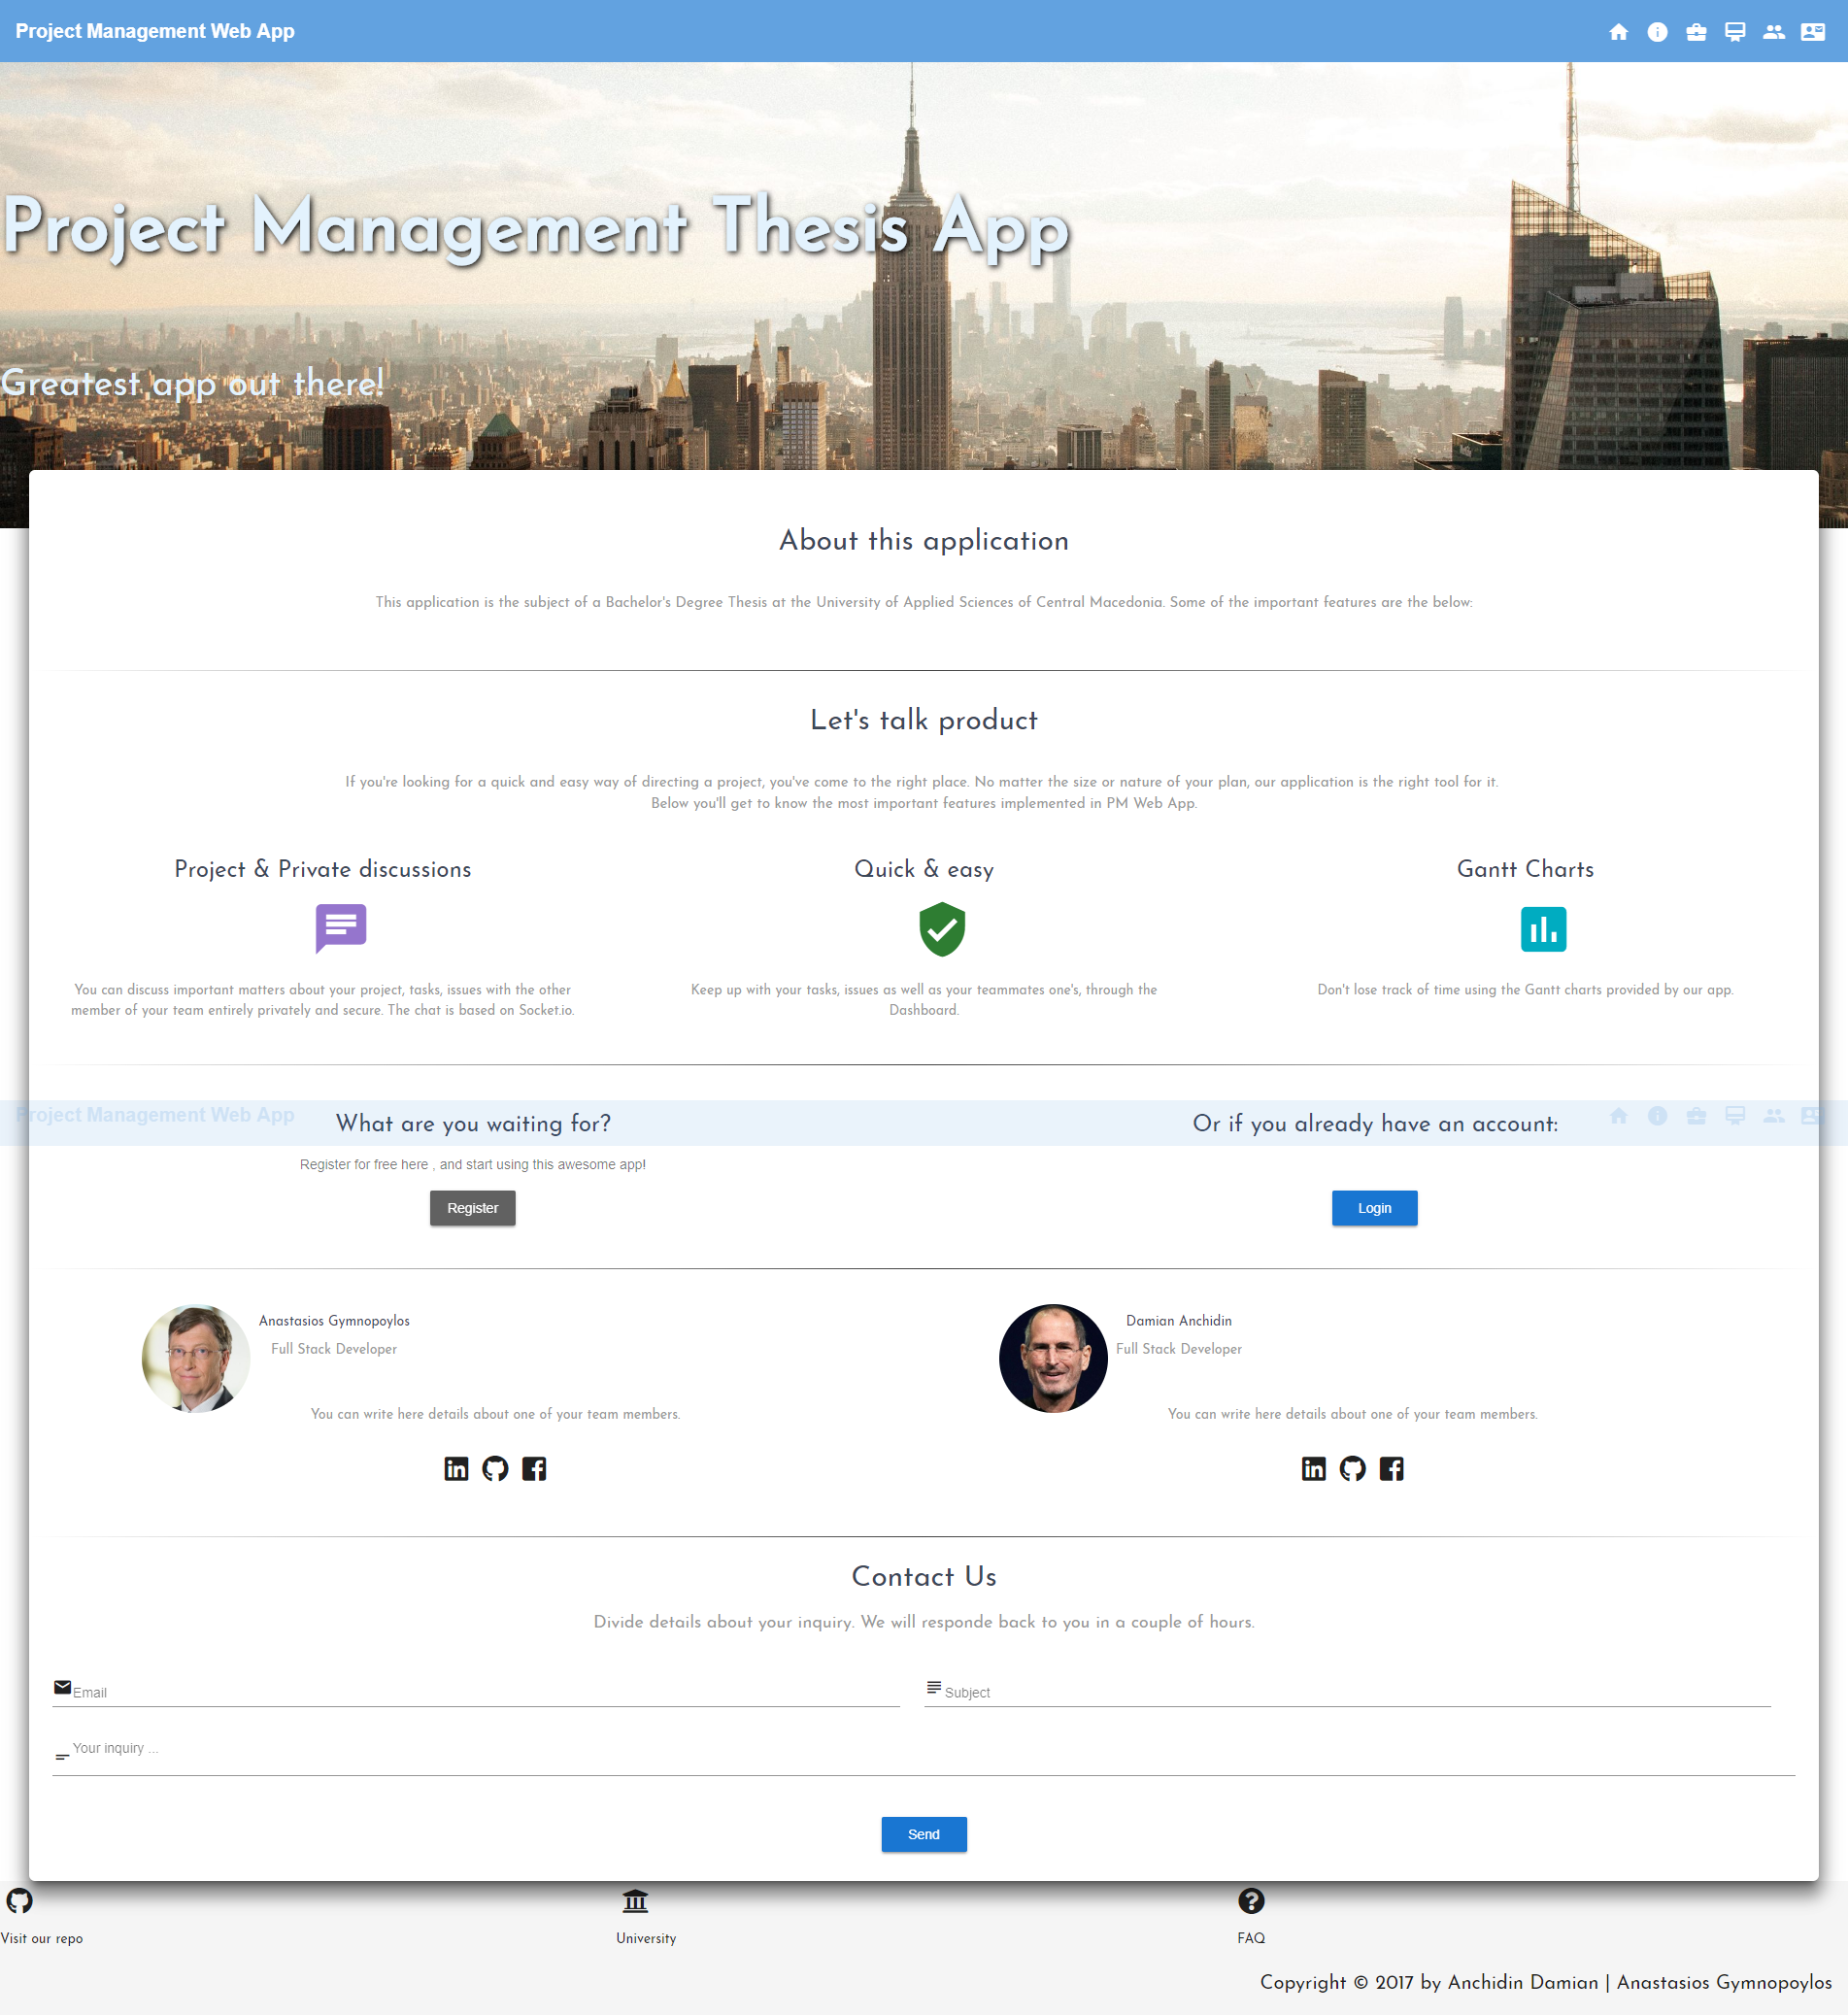
\includegraphics[scale=0.2]{images/homepage.png}
\caption{Αρχική σελίδα - \e{Homepage}}
\label{fig:homepage}
\end{figure}

\section{\e{Authentication}}
\pSpaceΉ εφαρμογή απαιτεί ένα λογαριασμό για να αποκτήσει ο χρήστης πρόσβαση στις υπηρεσίες που προσφέρονται.Ή εγγραφή αλλά και η είσοδος ολοκληρώνονται σε πολύ απλά βήματα.Προς το παρόν δεν υπάρχει δυνατότητα εγγραφής/ είσοδο με λογαρισμό κοινωνικού δικτύου.Αν ο χρήστης επιθυμεί να γυρίσει στην αρχική σελίδα, αυτό επιτυγχάνεται χρησιμοποιώντας την επιλογή του μένου που βρίσκεται στο πάνω μέρος της σελίδας. 

\subsection*{\e{Sign Up}}
\pSpaceΗ εγγραφή του χρήστη ακολουθεί μια βηματική μορφή για μια καλύτερη εμπειρία (βλ. σχ. \ref{fig:register}).\\
\pSpaceΤα βήματα πηγαίνουν ως εξής:\\
\begin{itemize}
	\item Αρχικά εμφανίζονται τρία πεδία για την ηλεκτρονική διεύθυνση, κωδικό και επαλήθευση κωδικού.Ο κώδικος πρέπει να έχει μήκος έξι χαρακτήρων και άνω, αλλιώς εμφανίζεται ένα σφάλμα που ενημερώνει τον χρήστη γι΄αυτήν την ιδιότητα.Επίσης υπάρχει δυνατότητα αποκάλυψης κωδικού για διευκολία.Ακόμη, σφάλματα σε περίπτωση που οι κωδικοί δεν είναι ίδιοι η αν η διεύθυνση δεν είναι έγκυρη εμφανίζονται σε πραγματικό χρόνο.Για να προχωρήσει στο επόμενο βήμα, δέν πρέπει να υπάρχουν σφάλματα ενεργά.
	\item Δύο ακόμη απαραίτητα πεδία υπάρχουν στο δεύτερο βήμα εγγραφής.Αφορούν το όνομα και το επίθετο του χρήστη.
	\item Στο τελευταίο βήμα, ο χρήστης έχει τρείς επιλογές: να γυρίσει στον προηγούμενο βήμα για να αλλάξει κάποιο πέδιο, \e{reset} φόρμας για να την ξανασυμπληρώσει και ολοκλήρωση διαδικασίας.
\end{itemize}
\pSpaceΑφού έχει ολοκληρωθεί με επιτυχία η εγγραφή του χρήστη, θα τον ανακατευθύνει στην σελίδα εισόδου.

\begin{figure}[!htb]
\centering
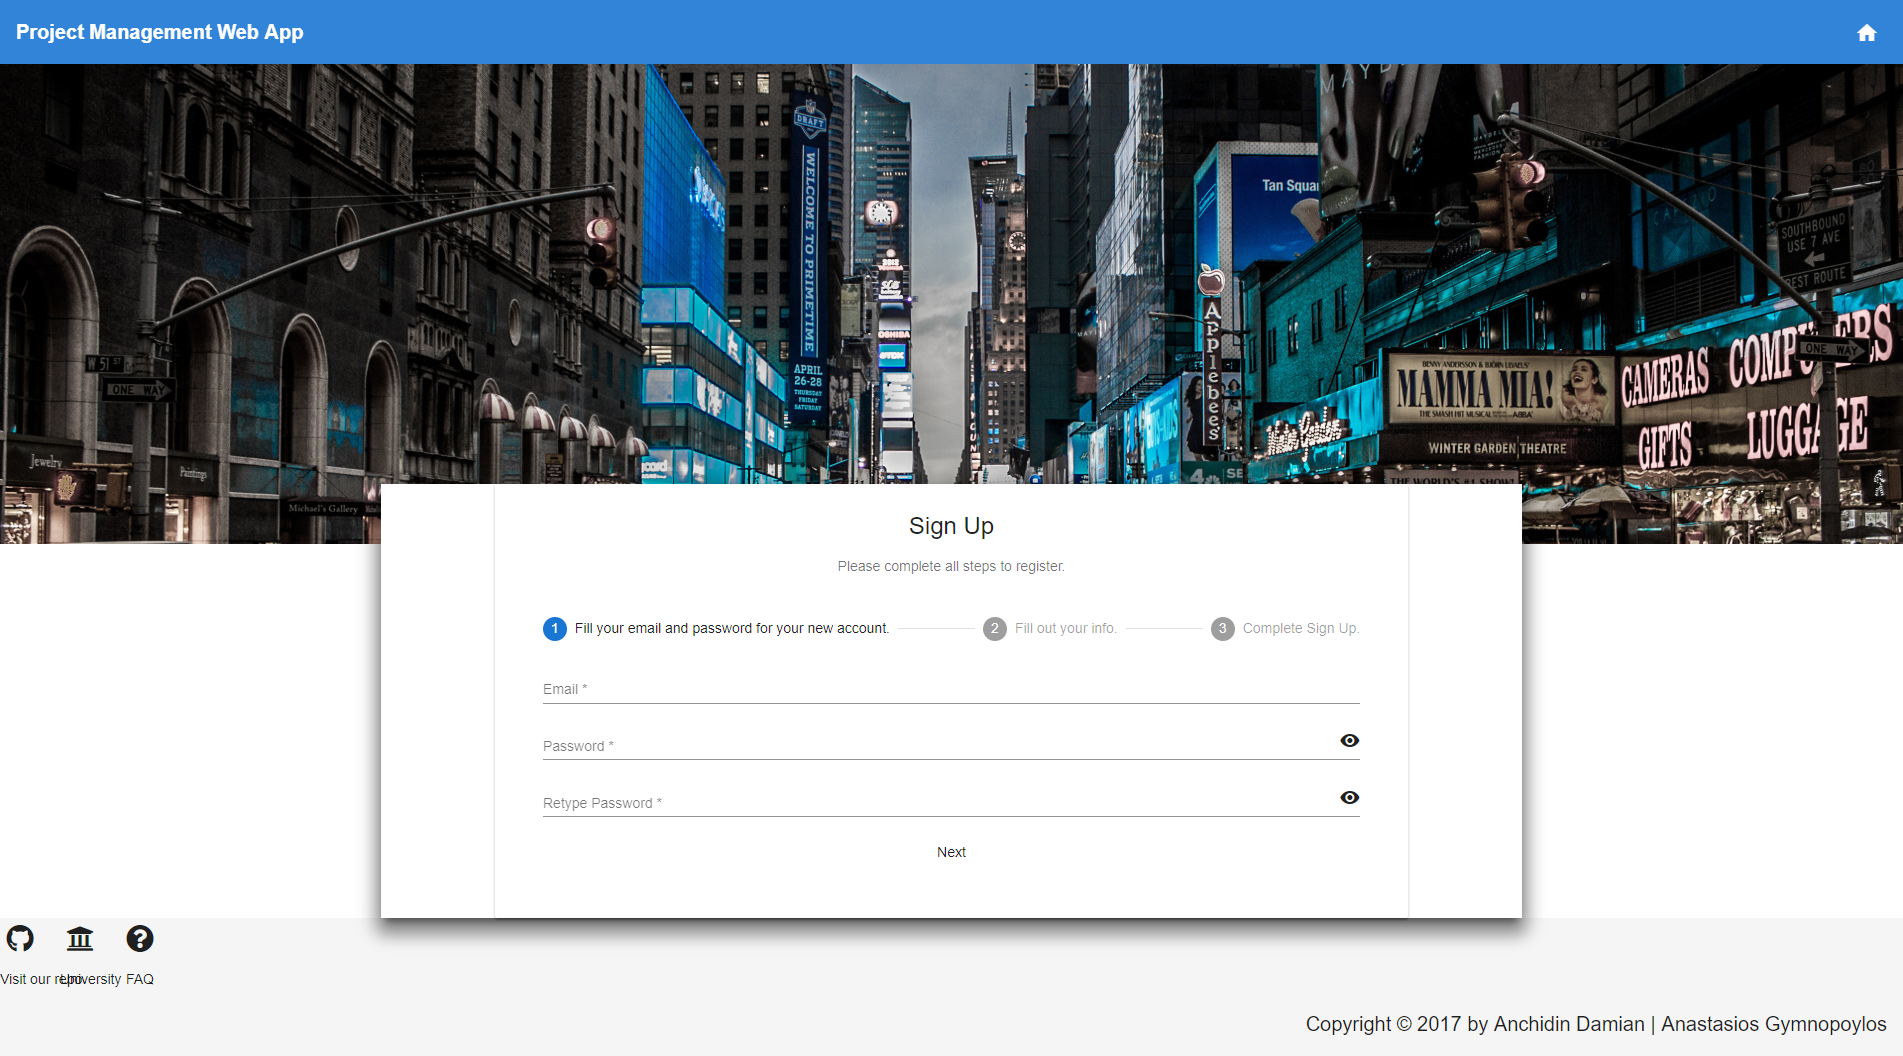
\includegraphics[scale=0.2]{images/register.png}
\caption{Εγγραφή - \e{Sign Up}}
\label{fig:register}
\end{figure}

\subsection*{\e{Sign In}}
\pSpaceΣυνηθίζεται για την είσοδο σε μια ηλεκτρονική υπηρεσία, να απαιτούνται μια ηλεκτρονική διεύθυνση και ένα κωδικό για επαλήθευση ταυτότητας.Τον ίδιο πρότυπο ακολυθείται και στην παρούσα εφαρμογή.\\
\pSpaceΟ χρήστης πληκτρολογεί το \e{email} και τον κωδικό, και σε περίπτωση απουσίας κάποιου σφάλματος, θα αποκτήσει πρόσβαση στις υπηρεσίες του \e{iPM}.Τα σφάλματα εμφανίζονται σε ένα \e{modal} παράθυρο με ένα μήνυμα που εξηγεί σε γενικές γραμμές το λάθος.Επίσης, όπως και στην εγγραφή, υπάρχει δυνατότητα αποκάλυψης κωδικού.Αν είναι επιτυχής η είσοδο, θα τον ανακατευθύνει στην εφαρμογή \e{iPM}.

\begin{figure}[!htb]
\centering
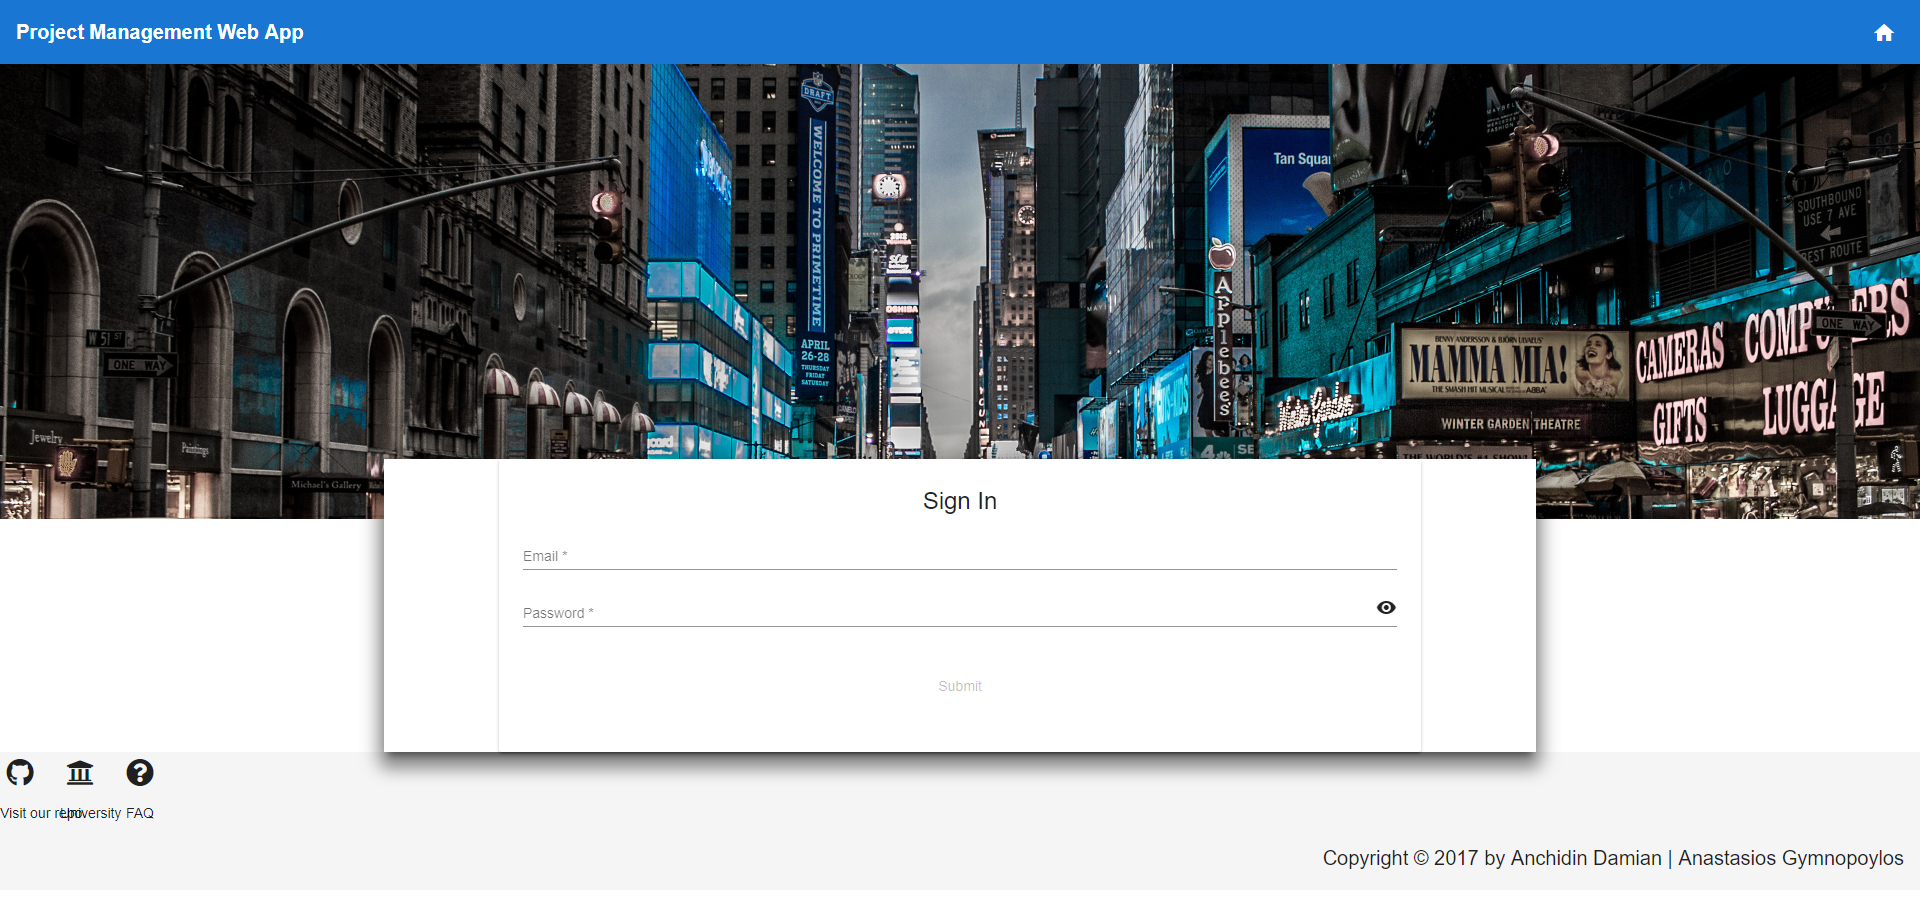
\includegraphics[scale=0.2]{images/login.png}
\caption{Είσοδο - \e{Sign In}}
\label{fig:login}
\end{figure}

\section{\e{iPM}}
\pSpaceΕφόσον έχει ολοκληρωθεί το στάδιο ταυτοποιήσης του χρήστη, θα αποκτήσει πρόσβαση στην διεύθυνση \e{\url{https://pmthesis.herokuapp.com/app}} όπου βρίσκεται η εφαρμογή \e{iPM}.Σημειώνεται πώς η εφαρμογή καταλαμβάνει αποθηκευτικό χώρο μέσω του \e{API} του περιηγητή, συγκεκριμένα το \e{Local Storage}.Αποθηκεύονται κάποιες ρυθμίσεις αλλά και το \e{token} που είναι απαραίτητο.Παρ'όλο που το \e{token} μπορεί να τον αποκωδικοποιήσει κανείς και να αλλάξει τις πληροφορίες του, μια τέτοια ενέργεια θα τον ακυρώσει με αποτέλεσμα να ανακατευθύνει τον χρήστη πάλι στην σελίδα εισόδου.Το ίδιο συμβαίνει και στην περίπτωση που λήγει η λείπει το παρόν \e{token}.\\
\pSpaceΗ σελίδα ακολουθεί τον ίδιο σχεδιασμό και στις δύο περιπτώσεις , χρήστη και έργο.Στο αριστερό μέρος υπάρχει το μενού με τις επιλογές που εξαρτώνται απο την ενότητα που βρίσκεται.Έχει την δυνατότητα απόκρυψης ώστε να μεγαλώσει ο χώρος δεδομένων.Στο επάνω μέρος, υπάρχουν κουμπιά που αφορούν τις ακόλουθες ενέργειες:\\
\begin{itemize}
	\item Το πρώτο στην σειρά είναι ένας διακόπτης για την απόκρυψη του αριστερού μενού.
	\item Δεύτερο είναι μια συντόμευση που επαναφέρει τον χρήστη στην αρχική σελίδα του \e{iPM}.
	\item Στην συνέχεια φαίνεται ένα πεδίο \e{Search} όπου ο χρήστης μπορεί να ψάξει έργα, άτομα και \e{task} για να διευκολυνθεί η διαχείριση έργων και εργασιών.
	\item Το επόμενο κουμπί εμφανίζει στο δεξίο μέρος της σελίδας τις ειδοποιήσεις.
	\item Ακολουθεί ένα κουμπί το όποιο ανοιγεί ένα μικρό \e{Context Menu} που περιέχει τέσσερις επιλογές για το θέμα σχεδιασμού.
	\item Τελευταίο είναι η αποσύνδεση, που ανακατευθύνει τον χρήστη στην σελίδα σύνδεσης.
\end{itemize}
\pSpaceΣτον υπόλοιπο χώρο φορτώνεται το δυναμικό περιεχόμενο.Θα αναφέρεται παρακάτω ως πλαίσιο δεδομένων.

% User actions
\subsection{\e{User}}
\pSpaceΑρχικά η εφαρμογή καλωσορίζει τον χρήστη, με τις ενέργειες που αφορούν τον ίδιο.Το μενού περιλαμβάνει τις ακόλουθες επιλογές, οι οποίες εξηγούνται σε λεπτομέρια παρακάτω:\\
\begin{itemize}
	\item \e{Dashboard}
	\item \e{My Projects}
	\item \e{My Tasks}
	\item \e{My Issues}
	\item \e{My Profile}
	\item \e{Calendar}
	\item \e{Chat}
	\item \e{Invites}
	\item \e{404}
\end{itemize} 

\subsubsection*{\e{Dashboard}}
\pSpaceΤο \e{Dashboard} (βλ. σχ. \ref{fig:userDashboard}) βρίσκεται στην διεύθυνση \e{\url{http://pmthesis.herokuapp.com/app/dashboard}} και φορτώνει στον πλαίσιο δεδομένων, πέντε καρτέλες:
\begin{itemize}
	\item Η πρώτη είναι μια δοκιμστική καρτέλα, στην οποία ο χρήστης αλλάζει το μέγεθος καρτέλων.
	\item Η δεύτερη εμφανίζει τα \e{Tasks} που είναι αναθετημένα στον ίδιο, στις οποίες έχει περάσει ο χρόνος ολοκλήρωσης.Προς το παρόν δείχνει μόνο απλά \e{Tasks}.
	\item Η επόμενη καρτέλα προσφέρει συντομεύσεις για τα ενεργά έργα.
	\item Στην τέταρτη καρτέλα, περιέχονται τα πι πρόσφατα \e{Tasks} που αναθέτηκαν στον χρήστη.
	\item Η τελευταία καρτέλα έχει την ίδια λειτουργία με την προηγούμενη, αλλά για τα \e{Issues}.
\end{itemize}

\pSpaceΣτις καρτέλες που περιέχουν τα \e{tasks, issues}, επιλέγοντας κάποιο απο αυτά, ανακατευθύνει τον χρήστη στην διεύθυνση \e{\url{https://pmthesis.herokuapp.com/app/assignmentview/@id}}.Επίσης η επιλογή ενός έργου απο την τρίτη καρτέλα, ανοίγει την ενότητα έργου με τις πληροφορίες του εν λόγω.

\begin{figure}[!htb]
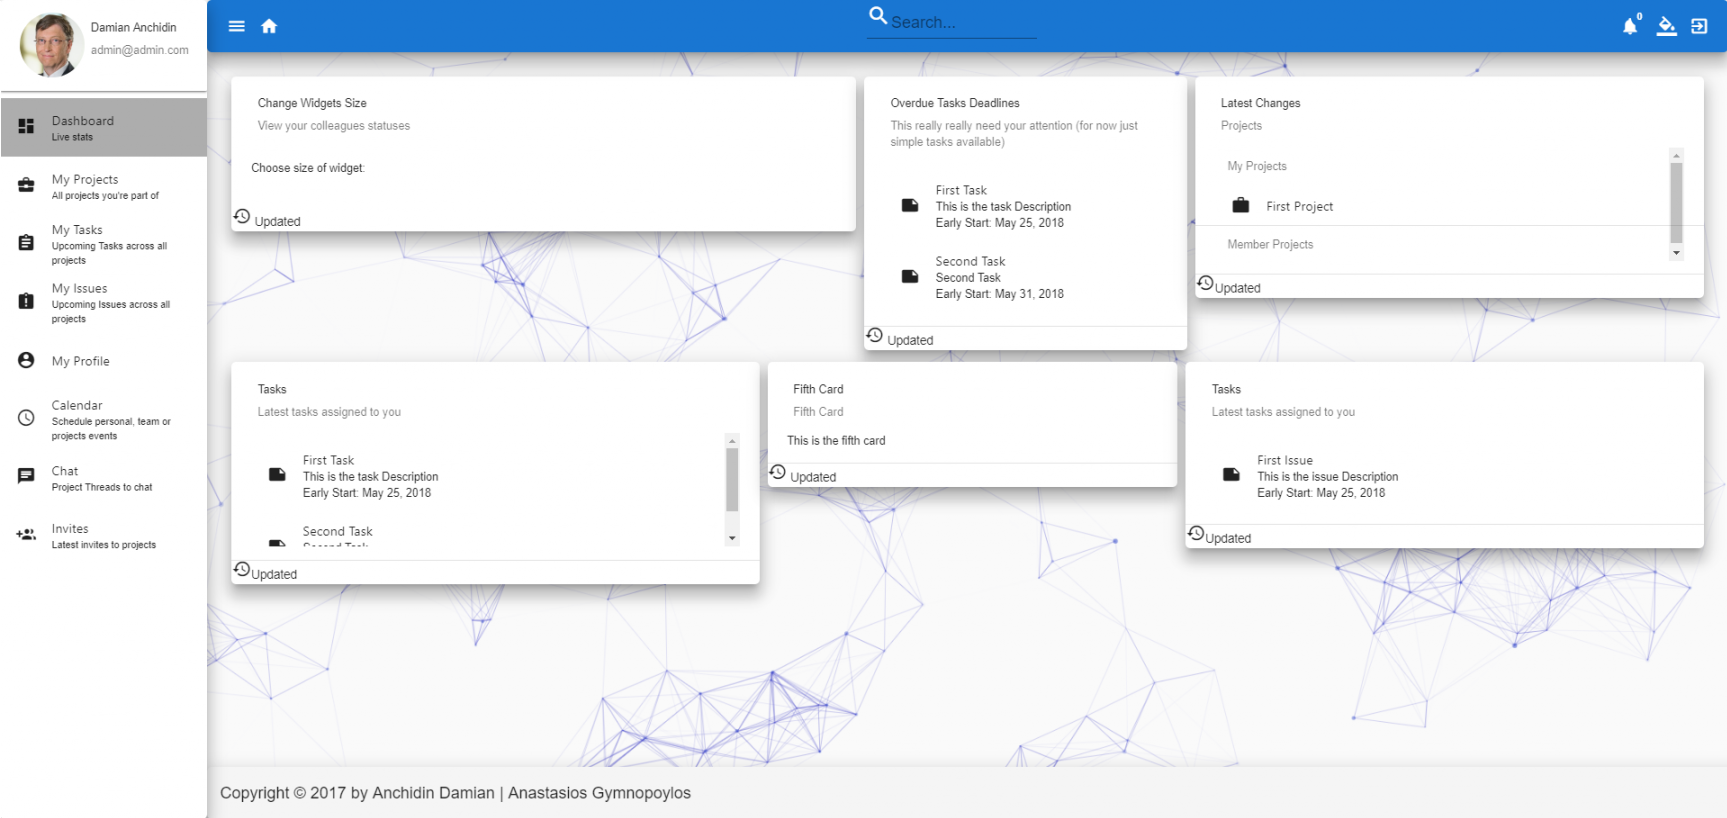
\includegraphics[width=\columnwidth, height=10cm]{images/userDashboard.png}
\caption{\e{User - Dashboard}}
\label{fig:userDashboard}
\end{figure}

\subsubsection*{\e{My Projects}}
\pSpaceΗ επιλογή \e{My Projects} από το αριστερό μενού της \e{iPM} φορτώνει στον πλαίσιο δεδομένων μια καρτέλα με τα ενεργά έργα του χρήστη (διαχειριστής η μέλος), αλλά και την δυνατότητα δημιουργίας νέου έργου.Η νέα διεύθυνση πλέον είναι \e{\url{https://pmthesis.herokuapp.com/app/myprojects}} (βλ. σχ. \ref{fig:userMyProjects}).

\begin{figure}[!htb]
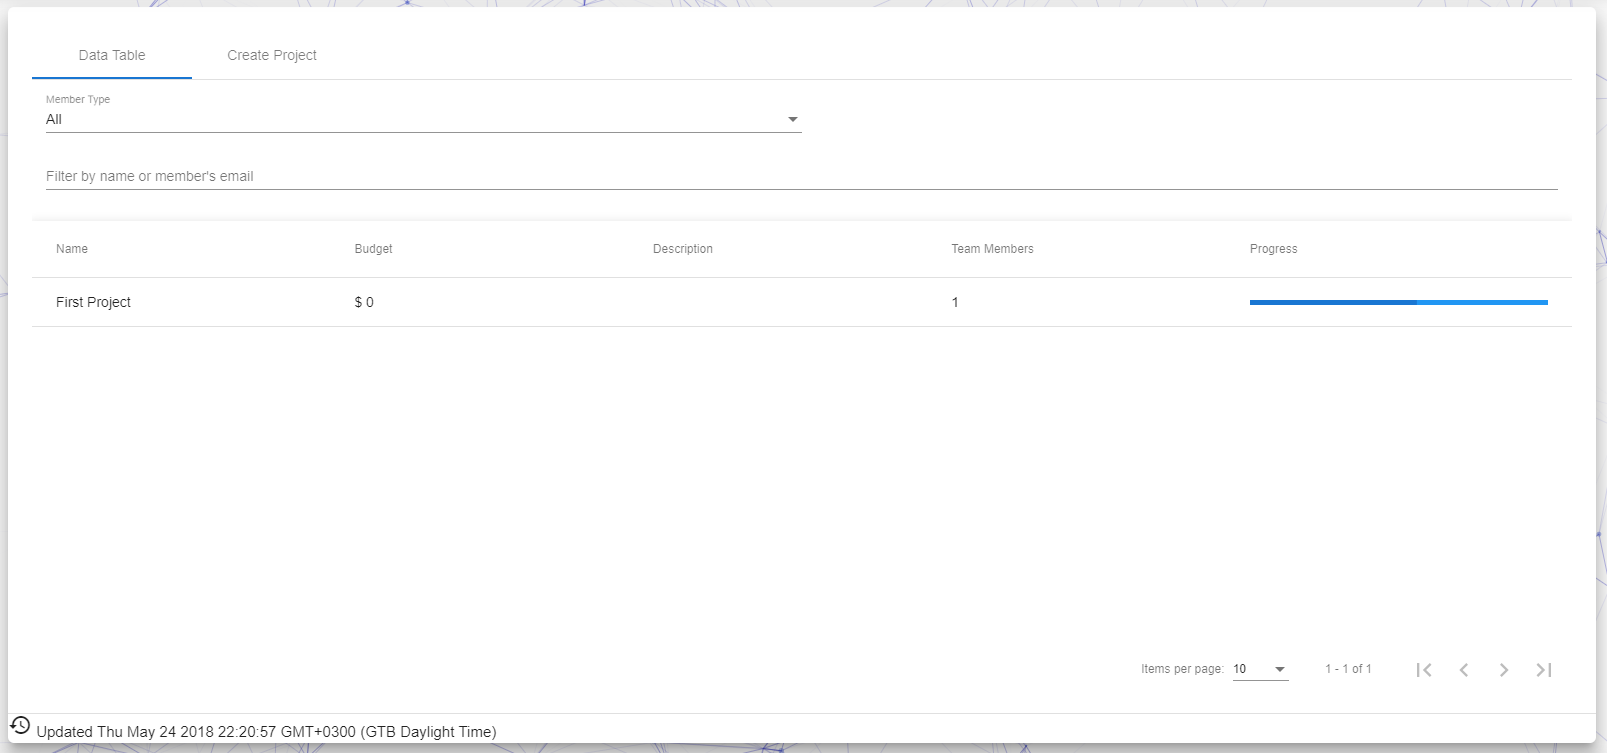
\includegraphics[width=\columnwidth, scale=4]{images/userMyProjects.png}
\caption{\e{User - My Projects}}
\label{fig:userMyProjects}
\end{figure}

\pSpaceΣτο πρώτο \e{tab} φαίνεται ο πίνακας με τα έργα του χρήστη. (σχ. \ref{fig:userMyProjects}).Κάθε εγγραφή αποτελείται από πέντε ιδιότητες: όνομα, προϋπολογισμός, μια σύντομη περιγραφή (εμφανίζονται μόνο 60 χαρακτήρες), μέγεθος ομάδας και η πρόοδο απεικονιζόμενη σε γραμμή πρόοδο.Επιλέγοντας κάποιο έργο, ανοίγει την "σελίδα" έργου.\\
\pSpaceΟ πίνακα διαθέτει σελιδοποίηση και ρύθμιση για τον σύνολο εγγραφών ανά σελίδα.Επιπλέον, πάνω από τον πίνακα υπάρχουν δύο πεδία που επιτρέπουν αλληλεπίδραση με τον χρήστη.\\
\pSpaceΤο πρώτο είναι τύπου \e{Select} και περιέχει τρείς επιλογές: \e{all, manager, member}, με την πρώτη να είναι η προκαθορισμένη.Σύμφωνα με την επιλεγμένη τιμή, ο πίνακας φιλτράρεται, εμφανίζοντας όλα τα έργα, έργα στα οποία ο χρήστης είναι διαχειριστής, η έργα στα οποία είναι μέλος.\\
\pSpaceΣτο δεύτερο πεδίο, ο χρήστης πληκτρολογεί ένα όνομα η μια ηλεκτρονική διεύθυνση και ο πίνακας φιλτράρεται με βάση αυτών.Σημειώνεται πώς τα δύο πεδία λειτουργούν ταυτοχρόνος, δηλαδή το αποτέλεσμα επηρεάζεται και απο τις δύο επιλογές.\\

\pSpaceΣυνεχίζοντας στον δεύτερο \e{tab}, \e{Create Project} (βλ. σχ. \ref{fig:userCreateProject1}), δίνεται η δυνατότητα δημιουργίας νέου έργου.Η λειτουργία αυτή ακολουθεί βηματική μορφή αποτελούμενο από τρία στάδια.\\
\pSpaceΣτο πρώτο βήμα, εισάγονται οι βασικές πληροφορίες του έργου, δηλαδή:\\
\begin{itemize}
	\item Η εταιρία που διαχειρίζει το εν λόγω έργο
	\item Τύπο έργο, ιδιωτικό η δημόσιο
	\item Όνομα έργου
	\item Προυπολογισμός
	\item Σύντομη περιγραφή
\end{itemize}

\begin{figure}[!htb]
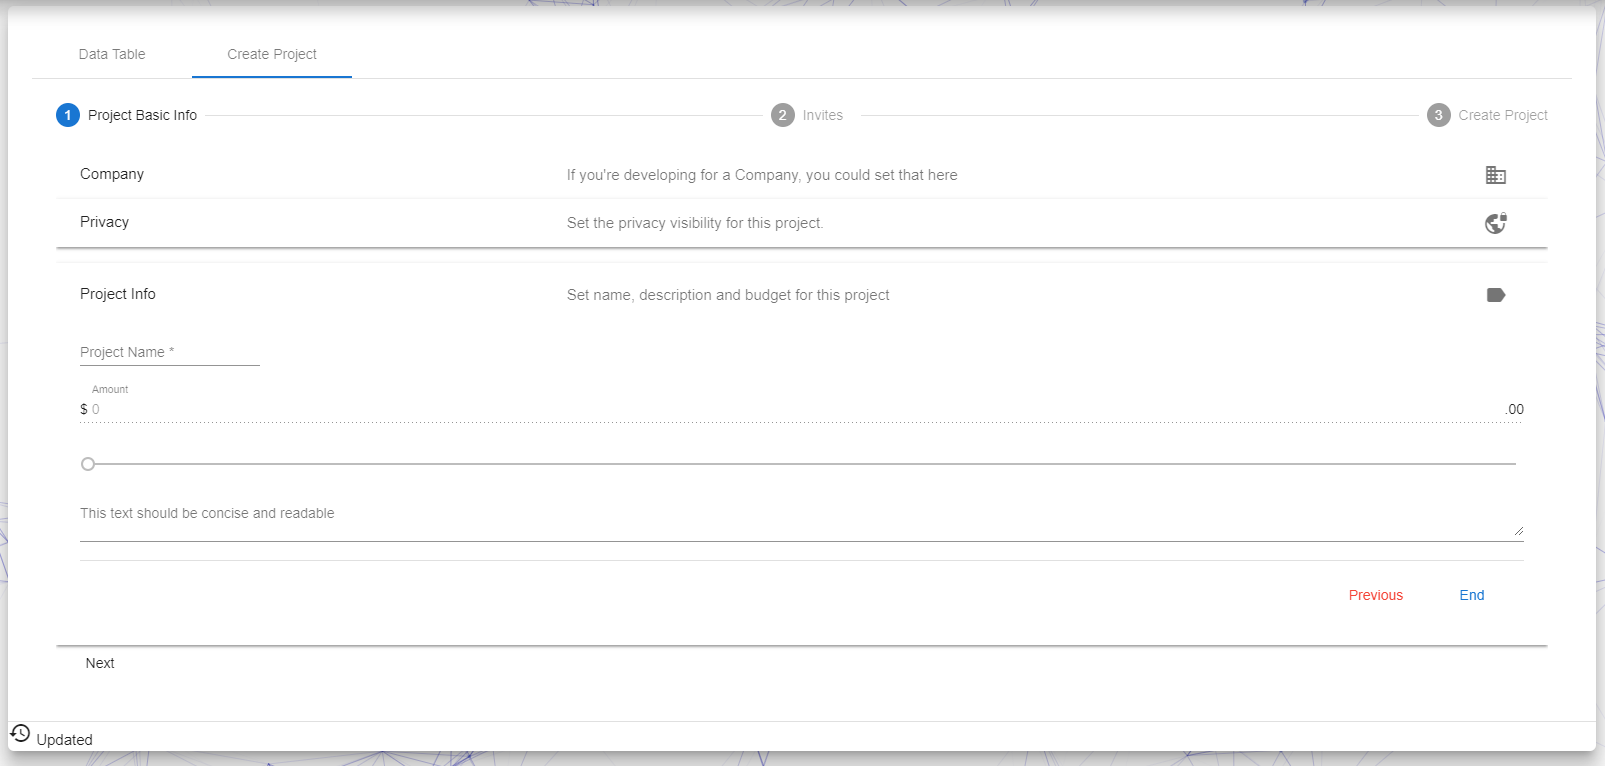
\includegraphics[width=\columnwidth, scale=4]{images/userCreateProject1.png}
\caption{\e{User - Create Project}}
\label{fig:userCreateProject1}
\end{figure}

\pSpaceΟ τύπος έργου, επιλέγεται με την βοήθεια ενός \e{Slide-Toggle}, και ο προυπολογισμός με έναν ολισθητή (\e{slider}) το οποίο έχει μέγιστη τιμή 50.000 .Τα υπόλοιπα είναι τα συνηθισμένα πεδία για εισαγωγή κειμένου.Για να περάσει στον επόμενο βήμα, είναι απαραίτητο να συμπληρωθεί το όνομα έργου.\\

\pSpaceΣτο δεύτερο βήμα (βλ. σχ. \ref{fig:userCreateProject2}), ο χρήστης μπορεί να καλέσει άτομα να συμβάλλουν στην ανάπτυξη έργου.Καθώς πληκτρολογεί μια ηλεκτρονική διεύθυνση στο πεδίο, εμφανίζονται απο κάτω \e{emails} υπαρκτών λογαριασμών.Επιλέγοντας κάποιο, τον προσθέτει στην λίστα προσκλήσεων.Επιπλέον, αν ο χρήστης πληκτρολογεί το κόμμα, προσθέτει αυτομάτως την διεύθυνση.Έτσι, αν οι διευθύνσεις είναι σωστές, η διαδικασία αυτή επιτυγχάνεται πιο γρήγορα.Ακόμη, αν ο χρήστης προσπαθεί να προσθέσει τον ίδιο, η λογαριασμοί που δεν υπάρχουν, εμφανίζεται ένα σφάλμα με μια σύντομη περιγραφή.

\begin{figure}[!htb]
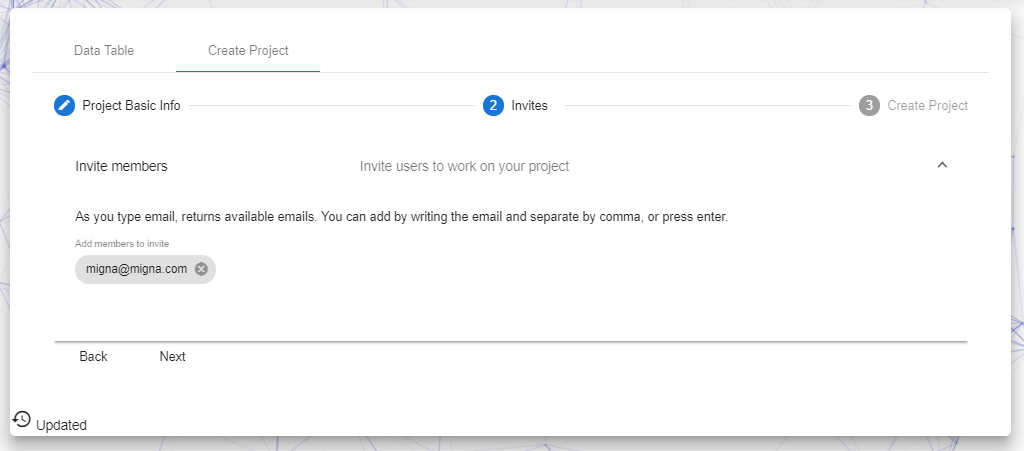
\includegraphics[width=\columnwidth, scale=4]{images/userCreateProject2.png}
\caption{\e{User - Create Project}}
\label{fig:userCreateProject2}
\end{figure}

\pSpaceΤο τελευταίο βήμα, εμφανίζει τις πληροφορίες του έργου που θα δημιουργηθεί αλλά και τρείς επιλογές: γύρισμα στο προηγούμενο βήμα, \e{reset} και ολοκλήρωση διαδικασίας.Αν ληφθεί επιτυχής μήνυμα, αλλάζει το \e{tab} στο αρχικό που εμφανίζονται τα έργα, όπου πλέον παρατηρείται και το καινούργιο.

\subsubsection*{\e{My Tasks}}
\pSpaceΟ χρήστης παρακολουθεί τα \e{Tasks} που του έχουν ανατεθεί, επιλέγοντας \e{My Tasks} από το αριστερό μενού η πηγαίνοντας στην διεύθυνση \e{\url{https://pmthesis.herokuapp.com/app/mytasks}}.Στο πλαίσιο δεδομένων, εμφανίζεται μια καρτέλα με ένα διάγραμμα (βλ. σχ. \ref{fig:userTasks}) που θυμίζει \e{Gantt}.\\
\pSpaceΗ εν λόγω διάγραμμα, περιέχει όλα τα \e{Tasks} που δεν έχουν ολοκληρωθεί, ανά έργο, σημειώντας και το διάστημα χρόνου τους.Για καλύτερη εμπειρία χρήσης, ένα έργο μπορεί να συρρικνωθεί σε περίπτωση που ο χρήστης θέλει να το αγνοήσει.\\
\pSpaceΕπιπλέον, το διάγραμμα προσφέρει την δυνατότητα εκτύπωσής της, η κατεβάσματος.Στην αριστερή γωνία, επιλέγοντας το κουμπί, ανοίγει ένα \e{Context Menu} με τέσσερις επιλογές: εκύπωση και κατέβασμα υπο διαφορετικές μορφές (\e{PNG, JPG, PDF, SVG}).

\begin{figure}[!htb]
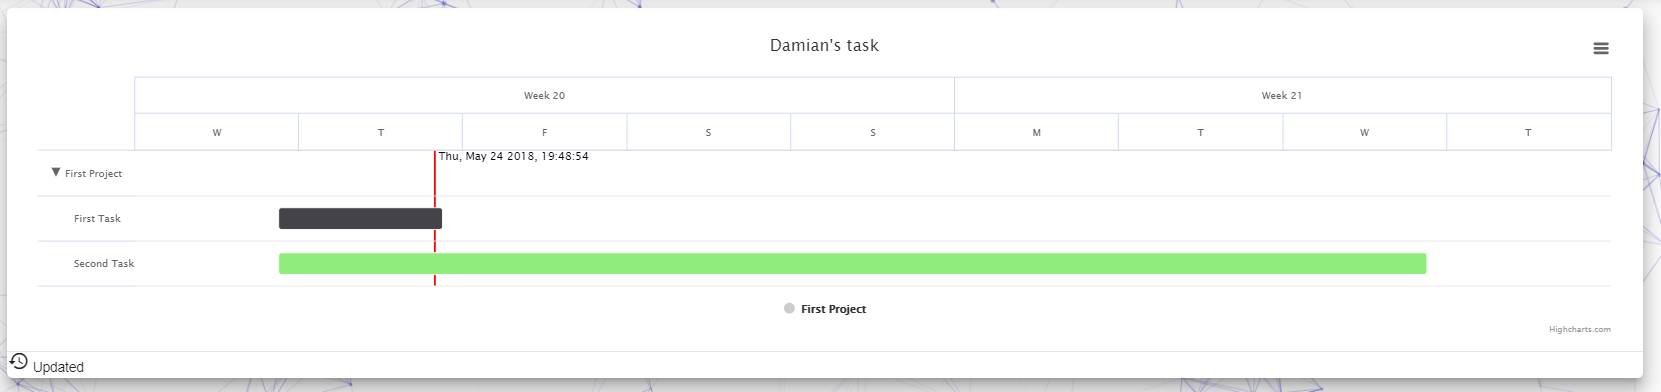
\includegraphics[width=\columnwidth, height=8cm]{images/userTasks.png}
\caption{\e{User - Tasks}}
\label{fig:userTasks}
\end{figure}

\subsubsection*{\e{My Issues}}
\pSpaceΠροχωρόντας στο \e{My Issues}, παρατηρείται ότι η καρτέλα (βλ. σχ. \ref{fig:userIssues}) που φορτώνεται στο πλαίσιο δεδομένων στην διεύθυνση \e{\url{https://pmthesis.herokuapp.com/app/myissues}}, είναι ίδια με την προηγούμενη (βλ. σχ. \ref{fig:userTasks}).Διαφέρουν στα δεδομένα που εμφανίζονται, καθώς εδώ υπάρχουν μόνο τα \e{Issues}, oι λειτουργίες όμως παραμένουν ίδιες.

\begin{figure}[!htb]
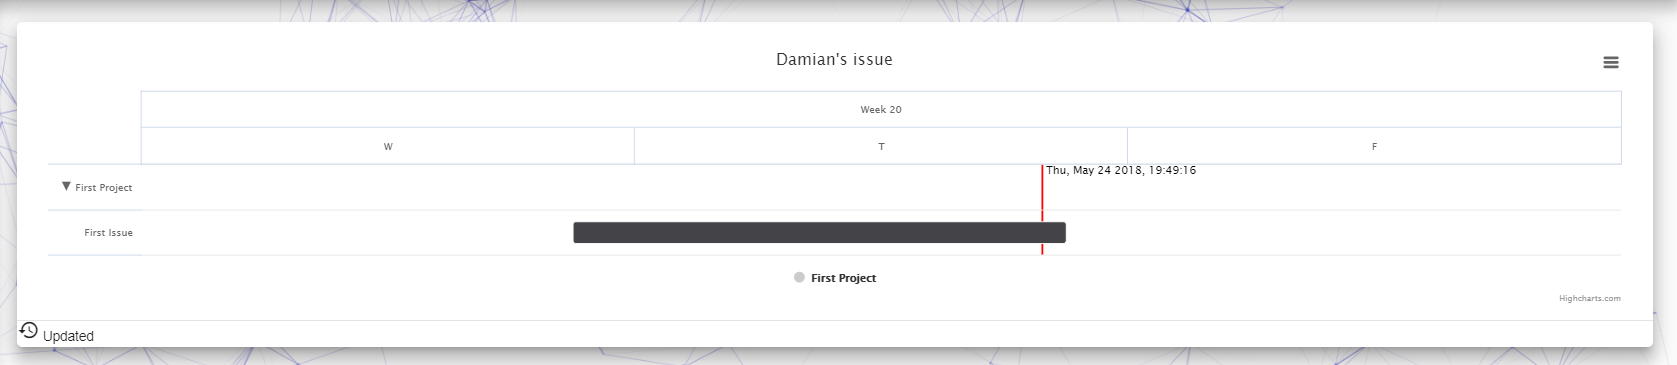
\includegraphics[width=\columnwidth, height=8cm]{images/userIssues.png}
\caption{\e{User - Issues}}
\label{fig:userIssues}
\end{figure}

\subsubsection*{\e{My Profile}}
\pSpaceΗ πέμπτη επιλογή του αριστερού μενού, \e{My Profile}, αλλάζει την διεύθυνση σε \e{\url{https://pmthesis.herokuapp.com/app/profile}} και φορτώνει στο πλαίσιο δεδομένων μια καρτέλα η οποία περιέχει τις πληροφορίες του χρήστη (βλ. σχ. \ref{fig:userProfile}).\\
\pSpaceΓια να πετύχει μια καλύτερη διοργάνωση των πληροφοριών και μια γρήγορη διαχείρισή τους ως αποτέλεσμα, προσθέτηκαν \e{Expansion Panels}, τα όποια κατέχουν ένα όνομα και μια σύντομη περιγραφή έτσι ώστε ο χρήστης να ανοίξει μόνο αυτό που επιθυμεί να αλλάξει η να δεί χωρίς να μετακινηθεί προς τα κάτω συνέχεια.\\
\pSpaceΥπάρχουν πέντε \e{Expansion Panels}:\\

\begin{figure}[!htb]
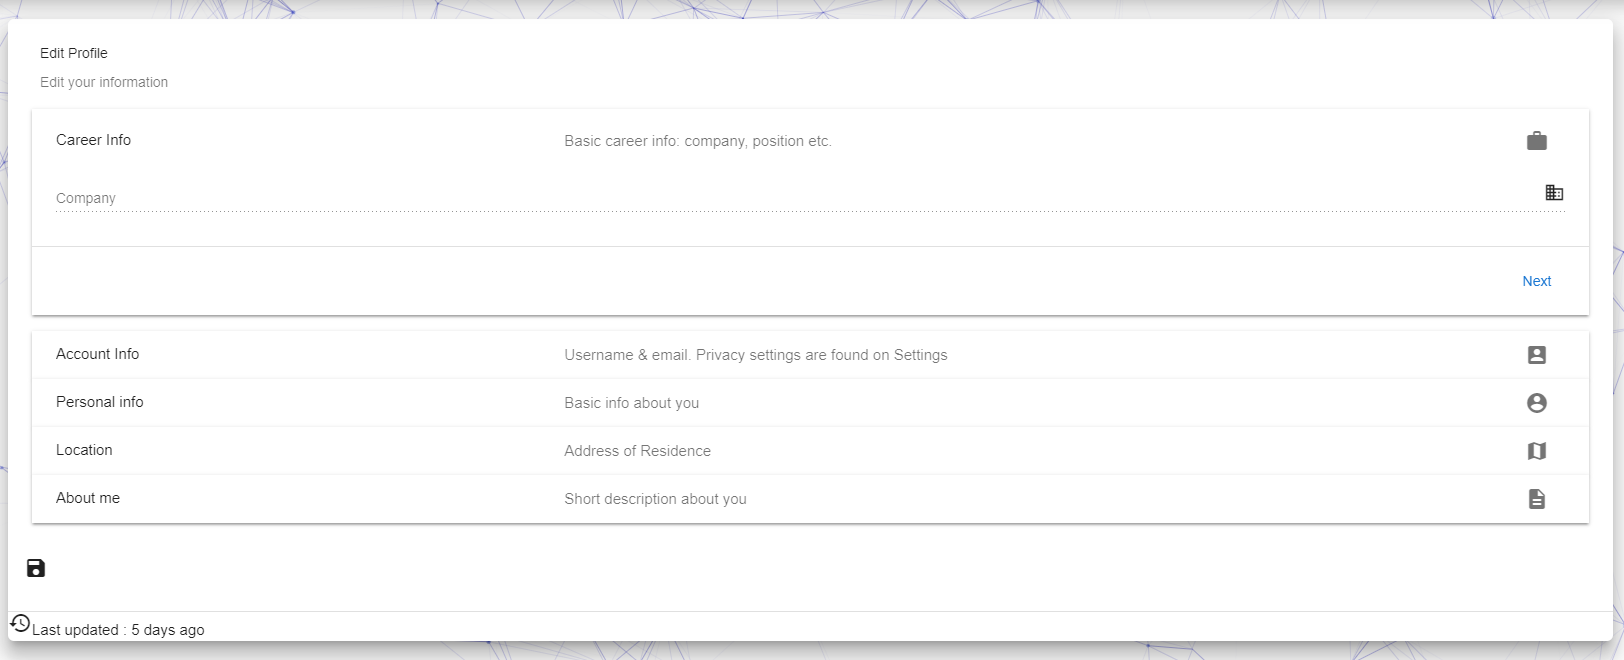
\includegraphics[width=\columnwidth, height=8cm]{images/userProfile.png}
\caption{\e{User - Profile}}
\label{fig:userProfile}
\end{figure}

\begin{itemize}
	\item \e{Career Info} - Προς το παρόν περιλαμβάνει ένα πεδίο όπου πληκτρολογείται η εταιρία στην όποια δουλεύει ο χρήστης.
	\item \e{Account Info} - Πληροφορίες που αφορούν τον λογαριασμό.Δύο πεδία κειμένου αποτελούν τον \e{panel} αυτό, ένα που αφορά την ηλεκτρονική διεύθυνση που δεν αλλάζει, και ένα για το \e{username} που επιθυμεί ο χρήστης να τον αντιπροσωπεύει.
	\item \e{Personal Info} - Δύο πεδία κειμένου επίσης και έδω, για το όνομα και το επίθετο του χρήστη.
	\item \e{Location} - Περιλαμβάνει τρία πεδία κειμένου για την διεύθυνση, πόλη, ταχυδρομικός κώδικας (μόνο αριθμητικύς χαρακτήρες) και ένα πεδίο τύπου \e{Select} όπου ο χρήστης μπορεί να επιλέξει την χώρα.Το τελευταίο πεδίο έχει την δυνατότητα αυτόματης συμπλήρωσης, δηλαδή καθώς πληκτρολογείται την ονομασία μιας χώρας, εμφανίζονται απο κάτω πιθανά αποτελέσματα μαζί με την σημαία (βλ. σχ. \ref{fig:userProfileCountry}).
	\item \e{About me} - Εδώ ο χρήστης μπορεί να περιγράψει τον εαυτό του σε ένα κείμενο μέγιστο μέγεθος 255 χαρακτήρων.Καθώς γράφει, στην δεξιά γωνία του πεδίου κειμένου, εμφανίζεται το τρέχων σύνολο χαρακτήρων.
\end{itemize}

\begin{figure}[!htb]
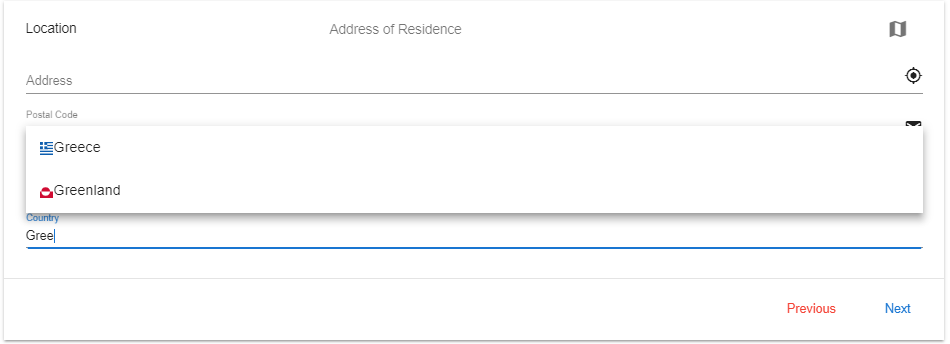
\includegraphics[width=\columnwidth, scale=4]{images/userProfileCountry.png}
\caption{\e{User - Select Country}}
\label{fig:userProfileCountry}
\end{figure}

\pSpaceΑν αποφασίσει να αλλάξει κάποιες από αυτές τις πληροφορίες ο χρήστης και επιθυμεί να τα αποθηκεύσει, αυτό επιτυγχάνεται με το κουμπί που βρίσκεται στην αριστερή γωνία της καρτέλας.\\
\pSpaceΕπιπλέον, υπάρχει και μια ακόμη διεύθυνση που αφορά το προφίλ ενός χρήστη \e{\url{https://pmthesis.herokuapp.com/app/profile/@email}}.Αντί για το \e{@email} ο χρήστης πληκτρολογεί την ηλεκτρονική διεύθυνση ενός υπαρκτού λογαριασμού.Οι πληροφορίες που εμφανίζονται είναι ελάχιστες προς το παρών.Ακόμη, αν πληκτρολογεί την δική του διεύθυνση, ανακατευθύνεται στην απλή διεύθυνση που αναφέραμε πιο πάνω.

\subsubsection*{\e{Calendar}}
\pSpaceΤο ημερολόγιο είναι ένα απο τα απαραίτητα εργαλεία στο \e{Project Management}.Η διεύθυνση \e{\url{https://pmthesis.herokuapp.com/app/calendar}} φορτώνει στο πλαίσιο δεδομένων μια καρτέλα που περιέχει ένα ημερολόγιο (βλ. σχ. \ref{fig:userCalendar}).\\
\pSpaceΠαρατηρείται πως στο πάνω μέρος της καρτέλας ύπάρχει μια ομάδα κουμπιών (\e{Month, Week, Day}), στην οποία μόνο ένα μπορεί να είναι επιλεγμένο ανα φορά.Απο κάτω, τρία κουμπιά (\e{Previous, Today, Next}) προσφέρουν την δυνατότητα περιήγησης (εξηγείται παρακάτω).\\
\pSpaceΕπιλέγοντας το \e{Month} η καρτέλα εμφανίζει τον τρέχων μήνα (βλ. σχ. \ref{fig:userCalendar}).Στις ημέρες που υπάρχουν σύμβαντα, το κελί της ημέρας δείχνει τον σύνολό τους, και αν επιλεχτεί η ημέρα, εμφανίζεται μια λίστα με τα σύμβαντα ανά κατηγορία.Τα τρία κουμπιά περιήγησης, σε αυτήν την περίπτωση δείχνουν τον προηγούμενο μήνα, τρέχων και επόμενο μήνα.

\begin{figure}[!htb]
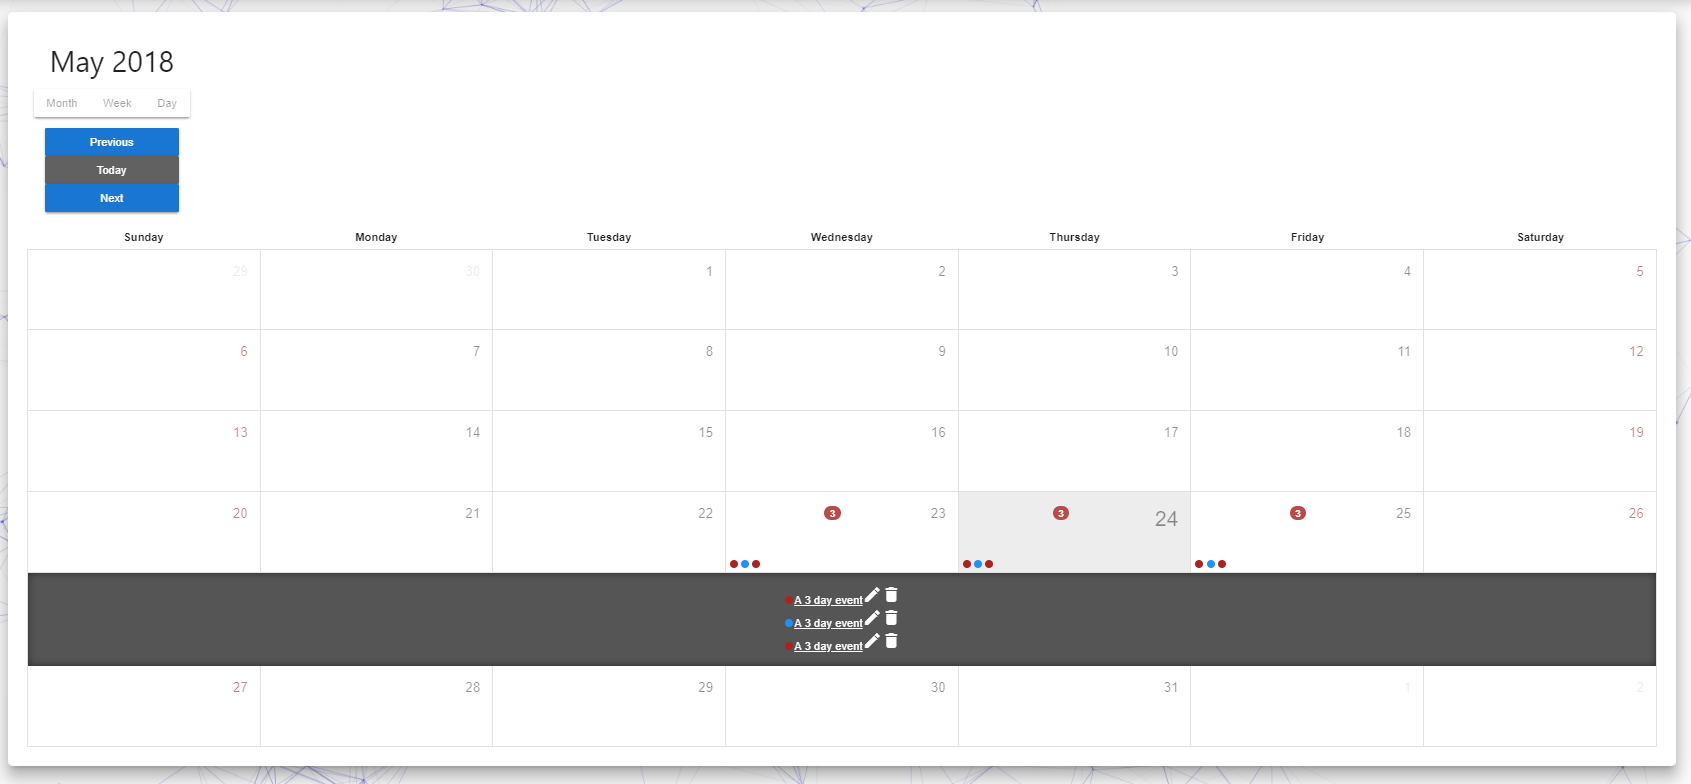
\includegraphics[width=\columnwidth, height=8cm]{images/userCalendar.png}
\caption{\e{User - Calendar Month}}
\label{fig:userCalendar}
\end{figure}

\pagebreak

\pSpaceΗ δεύτερη επιλογή της ομάδας κουμπιών, εμφανίζει την τρέχων εβδομάδα (βλ. σχ. \ref{fig:userCalendarWeek}).Τα κουμπιά περιήγησης, δείχνουν την προηγούμενη εβδομάδα, τρέχων και επόμενη.

\begin{figure}[!htb]
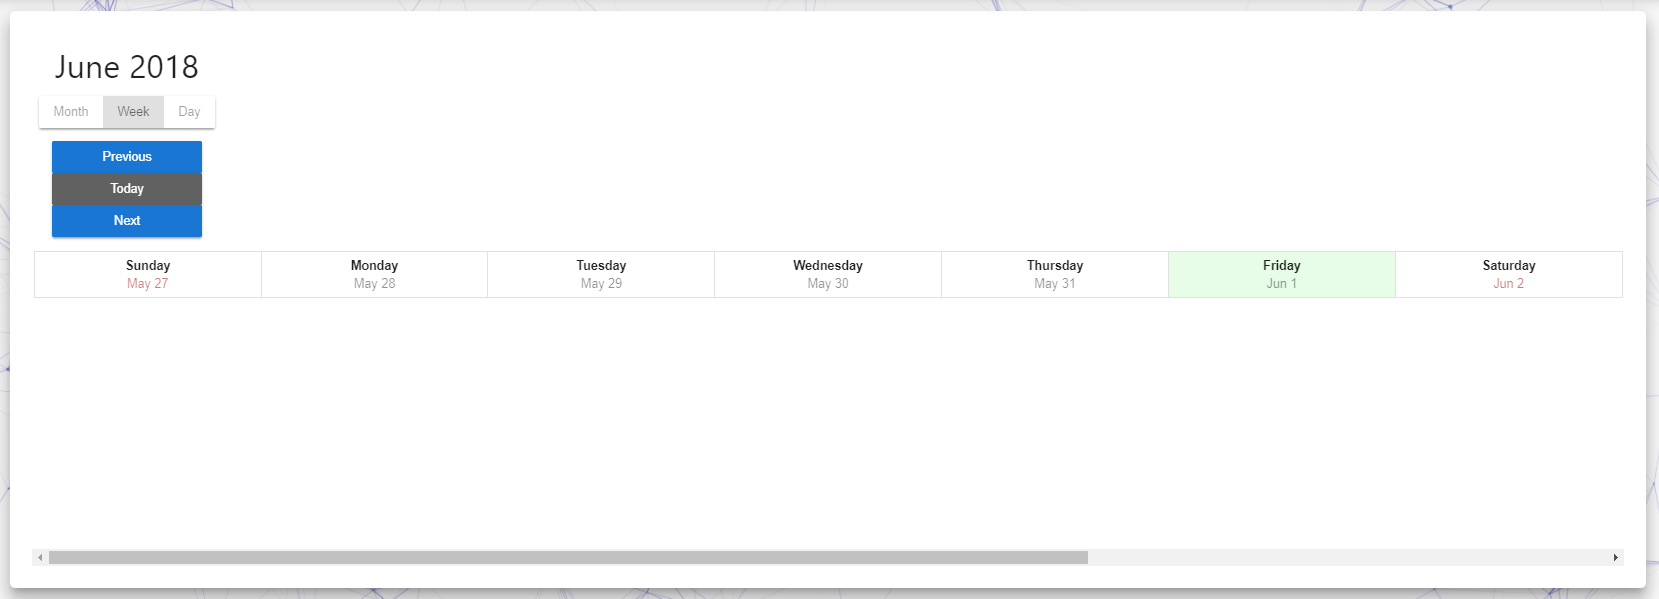
\includegraphics[width=\columnwidth, height=8cm]{images/userCalendarWeek.png}
\caption{\e{User - Calendar Week}}
\label{fig:userCalendarWeek}
\end{figure}

\pSpaceΗ τελευταία επιλογή , \e{Day}, εμφανίζει την τρέχων ημέρα (βλ. σχ. \ref{fig:userCalendarDay}) και τα κουμπιά περιήγησης δείχνουν την προηγούμενη μέρα, σημερινή και την επομένη.

\begin{figure}[!htb]
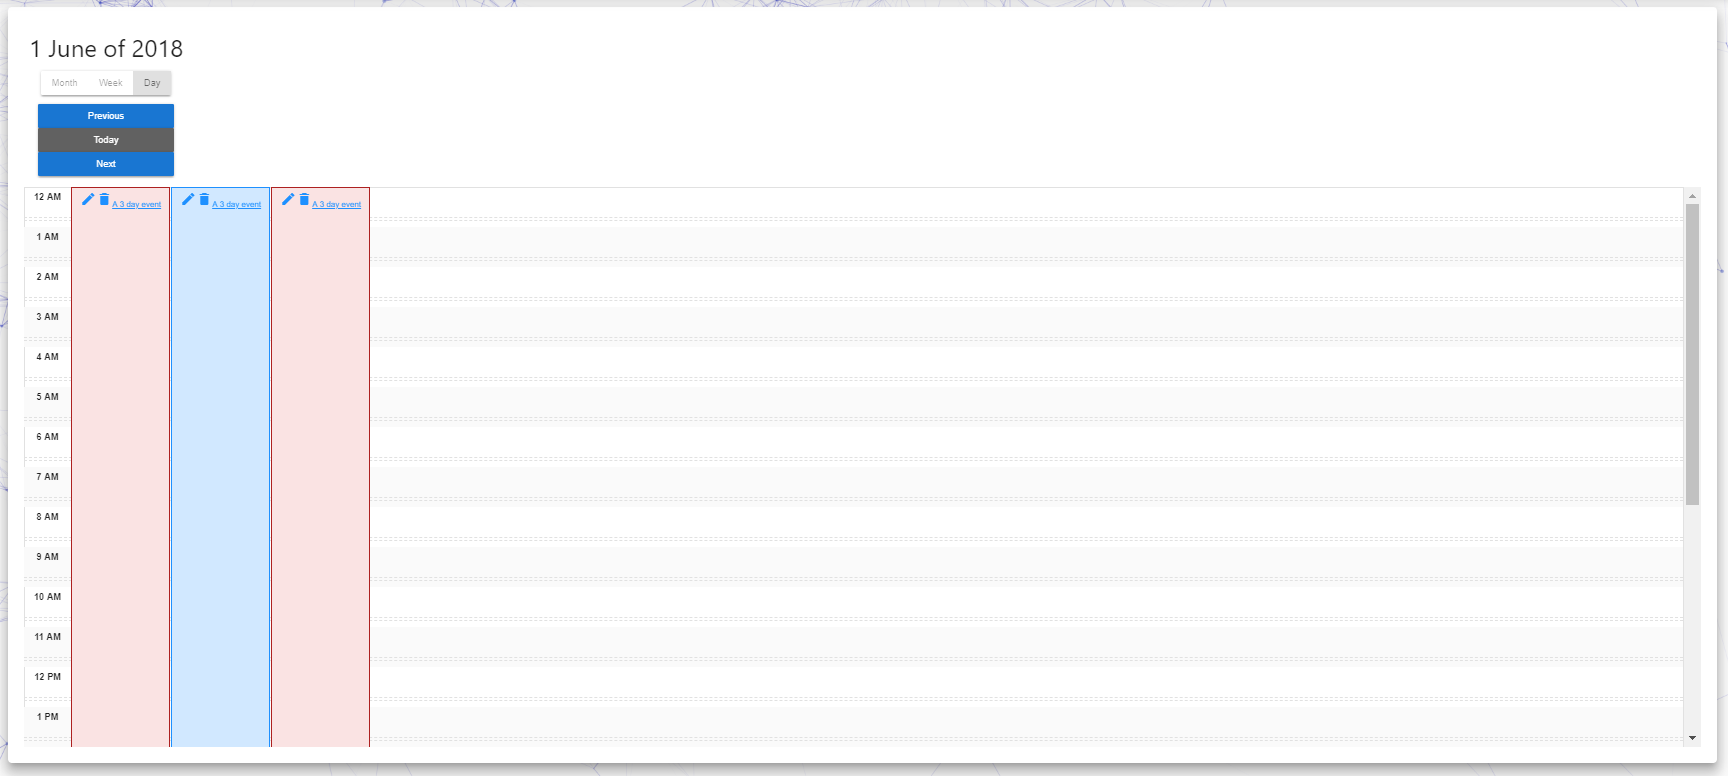
\includegraphics[width=\columnwidth, height=8cm]{images/userCalendarDay.png}
\caption{\e{User - Calendar Day}}
\label{fig:userCalendarDay}
\end{figure}

\pagebreak

\pSpaceΓια να προσθέσει ένα συμβάν στο ημερολόγιο, ο χρήστης πρέπει να επιλέξει την ημέρα που επιθυμεί, και ενεργοποιώντας το δεξί κλίκ επάνω της, εμφανίζεται ένα \e{Context Menu} με την επιλογή \e{Add Event}.Στην συνέχεια ανοίγει ένα \e{modal} παράθυρο (βλ. σχ. \ref{fig:userCalendarCreateEvent}).\\ \\
\pSpaceΌπως και στην καρτέλα προφίλ, για ευκολότερη διαχείριση, χρησιμοποιήθηκαν \e{Expansion Panels}.Στην παρούσα περίπτωση, τρία \e{panels} συμπεριλαμβάνονται στο παράθυρο \e{Create Event}:\\
\begin{itemize}
	\item \e{Info} - Υπάρχουν δύο πεδία, κειμένου και \e{select}.Το πρώτο αφορά τον τίτλο του σύμβαντα, ενώ το δεύτερο έχει ως επιλογές τα έργα του χρήστη.Με αυτόν τον τρόπο, σημειώνεται αν θα είναι προσωπικό η έργου.
	\item \e{Dates} - Δύο πεδία όπου ο χρήστης επιλέγει τις ημερομήνιες διεξαγωγής.
	\item \e{Type} - Ένα πεδίο \e{select} με τις επιλογές: \e{Danger, Info, Warning}.Ουσιαστικά εδώ ορίζει την κατηγορία στα οποία ανήκει, έτσι ώστε ο χρήστης να τα διακρίνει ευκολότερα. 
\end{itemize}

\begin{figure}[!htb]
\centering
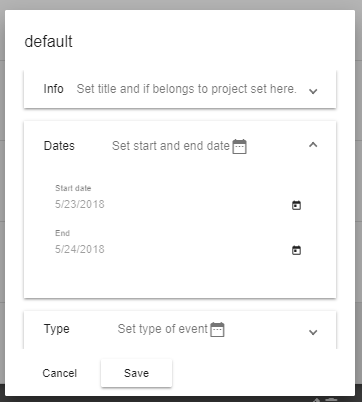
\includegraphics[scale=0.8]{images/userCalendarCreateEvent.png}
\caption{\e{User - Calendar Create Event}}
\label{fig:userCalendarCreateEvent}
\end{figure}

\pSpaceΠίσω στο ημερολόγιο, έχοντας επιλεγμένη μια μέρα (οποιοδήποτε \e{view mode}), ο χρήστης έχει την δυνατότητα να σέρνει κάποιο σύμβαν προς άλλη μέρα, η ώρα, και εφόσον το αφήσει εκεί που επιθυμεί, αποθηκεύεται η επεξεργασία ημερομηνιών.\\
\pSpaceΕπιπλέον, για περαιτέρων επεξεργασία, επιλέγοντας κάποιο συμβάν εμφανίζεται το ίδιο παράθυρο όπως του σχ. \ref{fig:userCalendarCreateEvent}.Ακόμη, είτε στην περίπτωση δημιουργίας είτε επεξεργασίας, αν η πρώτη ημερομηνία είναι μεγαλύτερη της δεύτερης, εμφανίζεται σφάλμα με μια σύντομη περιγραφή, όπως και αν λείπει ο τίτλος.Αν δέν διορθωθεί δεν είναι επιτυχής η αποθήκευση.

\subsubsection*{\e{Chat}}
\pSpaceΓια να πετύχει το \e{Project Management}, επιβάλλεται να υπάρχει καλή επικοινωνία στην ομάδα.Το \e{iPM} προσφέρει την δυνατότητα αυτή, σε χαμηλό επίπεδο, όσο για να συζητήσουν τα μέλοι μιας ομάδας κάποια θέματα.\\
\pSpaceΗ διεύθυνση \e{\url{https://pmthesis.herokuapp.com/app/chat}} φορτώνει στο πλαίσιο δεδομένων η καρτέλα του σχ. \ref{fig:userChat}.\\
\pSpaceΗ καρτέλα αποτελείται από:\\
\begin{itemize}
	\item Μενού με δυνατότητα απόκρυψης στα αριστερά.
	\item Γραμμη εργαλείων.
	\item Πλαίσιο συζήτησης.
	\item Γραμμη εργαλείων για αποστολή μηνύματος.
\end{itemize}

\pSpaceΣτο αριστερό μενού υπό τον υπότιτλο \e{Channels}, υπάρχει η λίστα έργων του χρήστη.Επιλέγοντας κάποιο από αυτά, θα εμφανίστουν όλα τα μηνύματα (βλ. σχ. \ref{fig:userChatMessage}) που ανήκουν στην συζήτηση το εν λόγω έργο, στο πλαίσιο συζήτησης.Σε αυτό το μενού, περιέχεται επίσης μια γραμμή εργαλείων, με ενέργειες για που αφορούν την διαθεσιμότητα του χρήστη, αλλά και ρυθμίσεις για το \e{Chat}.Αυτές οι ρυθμίσεις προς το παρόν, δεν είναι διαθέσιμα.\\
\pagebreak
\pSpaceΗ γραμμή εργαλείων, πάνω απο τον πλαίσιο συζήτησης, περιέχει έναν διακόπτη για την απόκρυψη του αριστερού μενού και τον τίτλο της συζήτησης, το οποίο συμβαίνει να είναι ο τίτλος του έργου.\\
\pSpaceΚάτω απο τον πλαίσιο συζήτησης, παρατηρείται η γραμμή εργαλείων για την αποστολή μηνυμάτων στο τρέχων \e{channel thread}.Δεν υπάρχει περιορισμό χαρακτήρων για το μήνυμα που θα σταλθεί.\\

\begin{figure}[!htb]
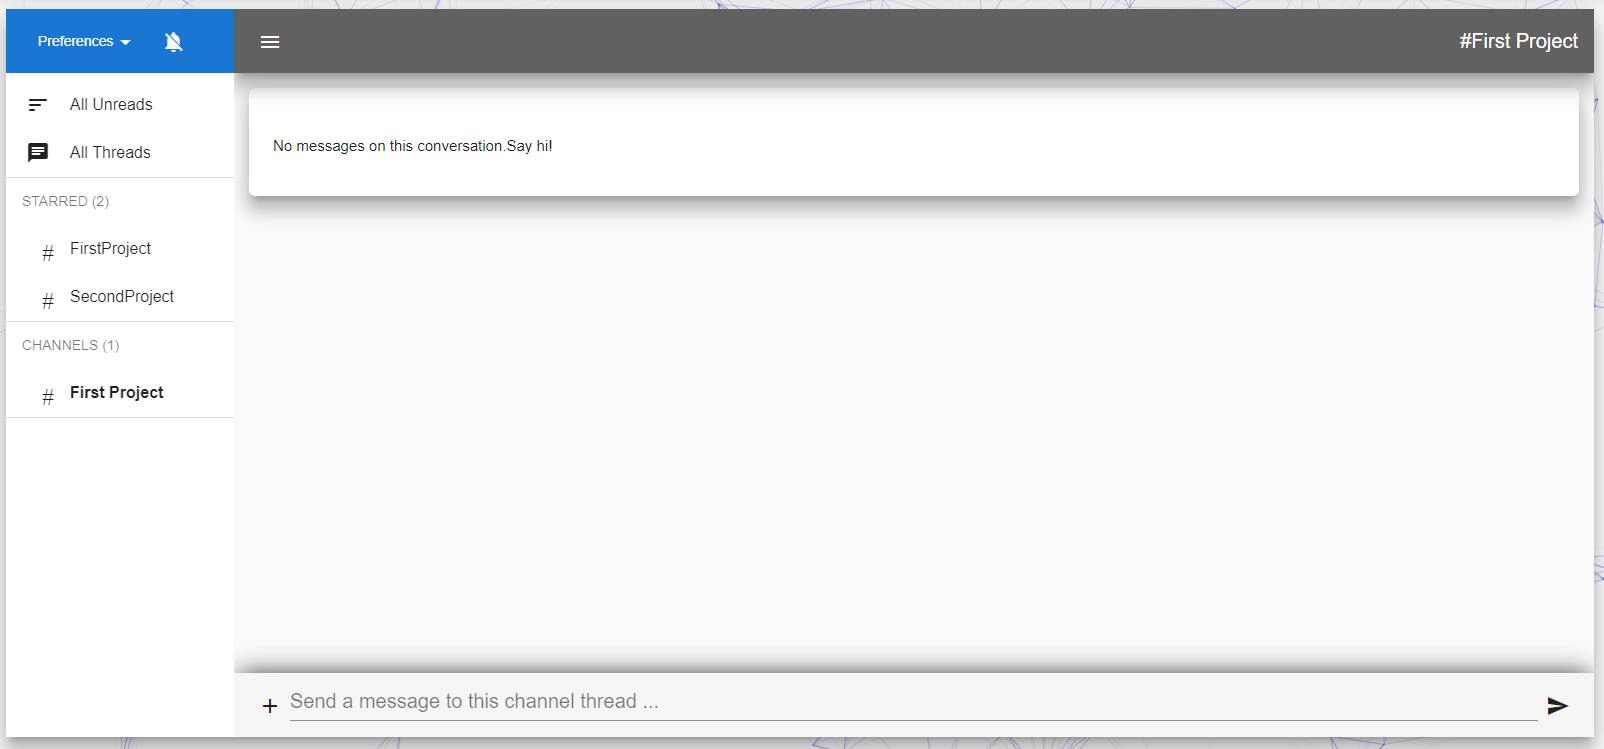
\includegraphics[width=\columnwidth, height=10cm]{images/userChat.png}
\caption{\e{User - Chat}}
\label{fig:userChat}
\end{figure}

\begin{figure}[!htb]
\centering

\includegraphics[width=\linewidth]{images/userChatMessage.png}
\caption{\e{User - Chat Message}}
\label{fig:userChatMessage}
\end{figure}

\subsubsection*{\e{Invites}}
\pSpaceΓια να συμβάλλει ένας χρήστης σε κάποιο έργο, θα χρειαστεί να τον προσκαλέσει κάποιο μέλος το έργου έν λόγω.Οι προσκλήσεις είναι διαθέσιμες στην διεύθυνση \e{\url{htts://pmthesis.herokuapp.com/app/invites}}, η οποία φορτώνει την καρτέλα του σχ. \ref{fig:userInvites}.\\
\pSpaceΑπεικονίζεται έναν πίνακα, στον οποίο, η εγγραφές έχουν την ακόλυθη μορφή: αριθμό, τίτλος έργου, και 2 ενέργειες αποδοχή και απόρριψη.

\begin{figure}[!htb]
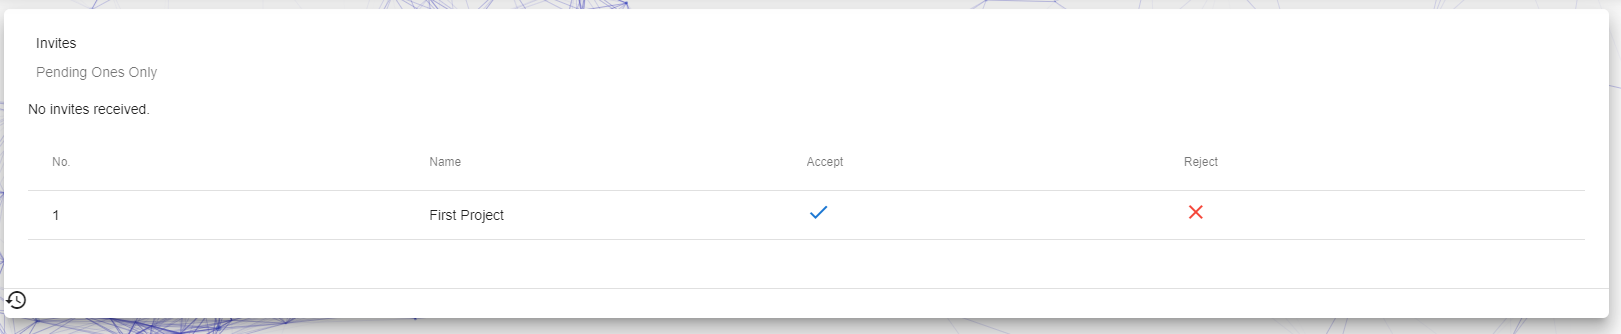
\includegraphics[width=\linewidth]{images/userInvite.png}
\caption{\e{User - Invites}}
\label{fig:userInvites}
\end{figure}

\subsubsection*{\e{404}}
\pSpaceΚάποιες φορές είτε κατα λάθος, είτε σκόπιμα, ο χρήστης πληκτρολογεί μια διεύθυνση η οποία δεν υπάρχει.Για την αποφυγή προβλημάτων, σφαλμάτων, υπάρχει μια διεύθυνση, η οποία φορτώνεται αυτόματα όταν η διεύθυνση που πληκτρολογήθηκε είναι λανθασμένη.Ανακατευθύνεται στην διεύθυνση \e{\url{https://pmthesis.herokuapp.com/app/404}} η οποία φορτώνει μια καρτέλα (βλ. σχ. \ref{fig:404}) στην οποία υπάρχει μια σύντομη περιγραφή του σφάλματος αλλά και την δυνατότητα να ψάξει για κάτι έτσι ώστε να μην ξαναφτάσει σε ίδια θέση.

\begin{figure}[!htb]

\includegraphics[width=\linewidth]{images/404.png}
\caption{\e{404}}
\label{fig:404}
\end{figure}

% /User actions

\pagebreak

% Project actions
\subsection{\e{Project}}
\pSpaceΣτην ενότητα έργου, υπάρχουν δύο διαφορές: το αριστερό μενού και η διεύθυνση.Το αριστερό μενού περιλαμβάνει τις ακόλυθες επιλογές:\\
\begin{itemize}
	\item \e{Dashboard}
	\item \e{Assignments}
	\item \e{Gantt}
	\item \e{Team}
	\item \e{Action Log}
	\item \e{Chat}
	\item \e{Settings}
\end{itemize}
\pSpaceΌλες εξηγούνται παρακάτω, εκτός του \e{Chat}, το οποίο παραμένει ίδιο με αυτό που έχει αναφερθεί ήδη στην ενότητα \e{User}.\\
\pSpaceΕπίσης, σημειώνεται πως όλα τα δεδομένα πλέον αφορούν το έργο.

\subsubsection*{\e{Dashboard}}
\pSpaceΑνοίγωντας κάποιο έργο, ο χρήστης θα συναντήσει πρώτα το \e{Dashboard} (βλ. σχ. \ref{fig:projectDashboard}) στην διεύθυνση \e{\url{https://pmthesis.herokuapp.com/app/project/dashboard}}.Φορτώνονται τέσσερις καρτέλες (δύο είναι μη διαθέσιμα προς το παρόν).Τα δύο που είναι ενεργά, έχουν τον ίδιο σχεδιασμό και λειτουγία, αλλα διαφορετικά δεδομένα:
\begin{itemize}
	\item Η πρώτη καρτέλα δείχνει τα στατιστικά για τα \e{Tasks}.
	\item Η δεύτερη απεικονίζει τα στατιστικά για τα \e{Issues}.
\end{itemize}

\begin{figure}[!htb]
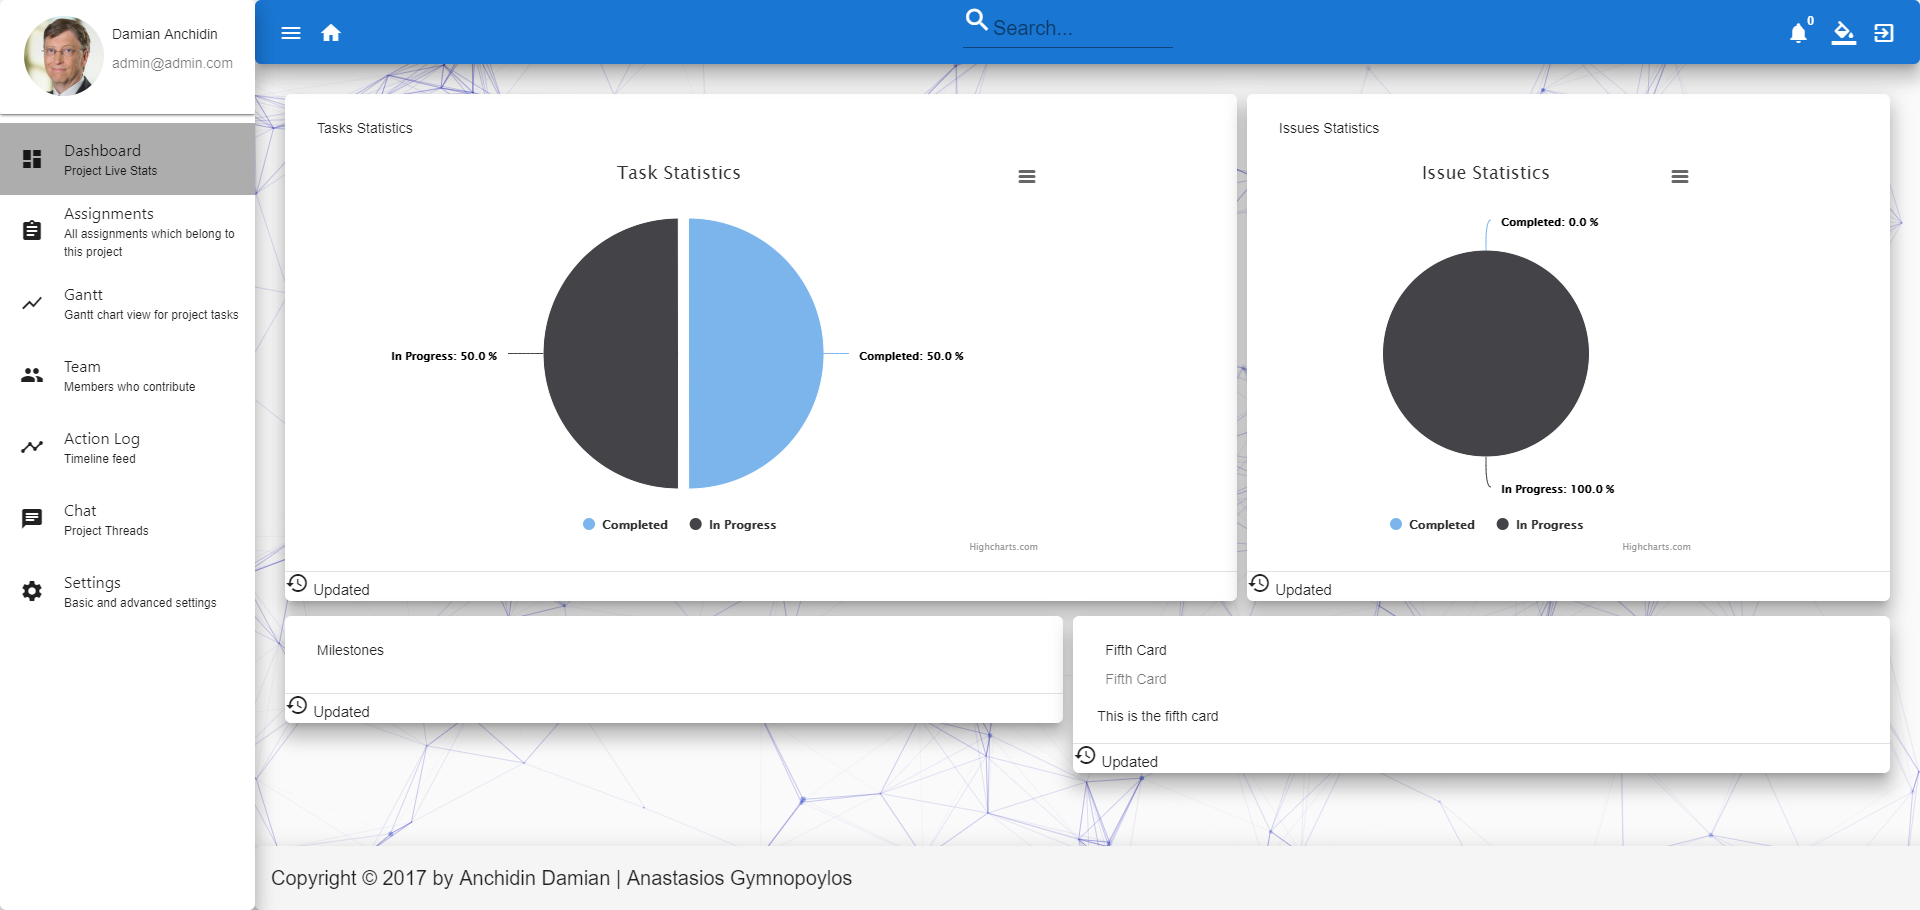
\includegraphics[width=\linewidth]{images/projectDashboard.png}
\caption{\e{Project - Dashboard}}
\label{fig:projectDashboard}
\end{figure}

\pSpaceΚαι στις δύο περιπτώσεις, χρησιμοποιήθηκαν διαγράμματα σε μορφή πίτας (\e{Pie Chart}).Όπως όλα τα διαγράμματα της εφαρμογής, προσφέρουν την δυνατότητα εκτύπωσης και κατεβάσματος.Επιπλέον, σε περίπτωση που δεν υπάρχουν δεδομένα, το διάγραμμα εξαφανίζεται, και μένει μια συντόμευση που οδηγεί τον χρήστη στην δημιουργία \e{Tasks} και \e{Issues}.

\pagebreak

\subsubsection*{\e{Assignments}}
\pSpaceΗ ανάθεση εργασιών στα μέλοι του έργου, είναι μια απο τις βασικότερες έννοιες του \e{Project Management}.Στην εφαρμογή \e{iPM} αυτό αλλά και η διαχείρισή τους επιτυγχάνεται από την επιλογή \e{Assignments} του αριστερού μενού, που αδηγεί στην διεύθυνση \e{\url{https://pmthesis.herokuapp.com/app/project/assignments}}.Αυτό φορτώνει μια καρτέλα η οποία είναι η βάση για το υπόλοιπα (βλ. σχ. \ref{fig:projectAssignments})

\begin{figure}[!htb]
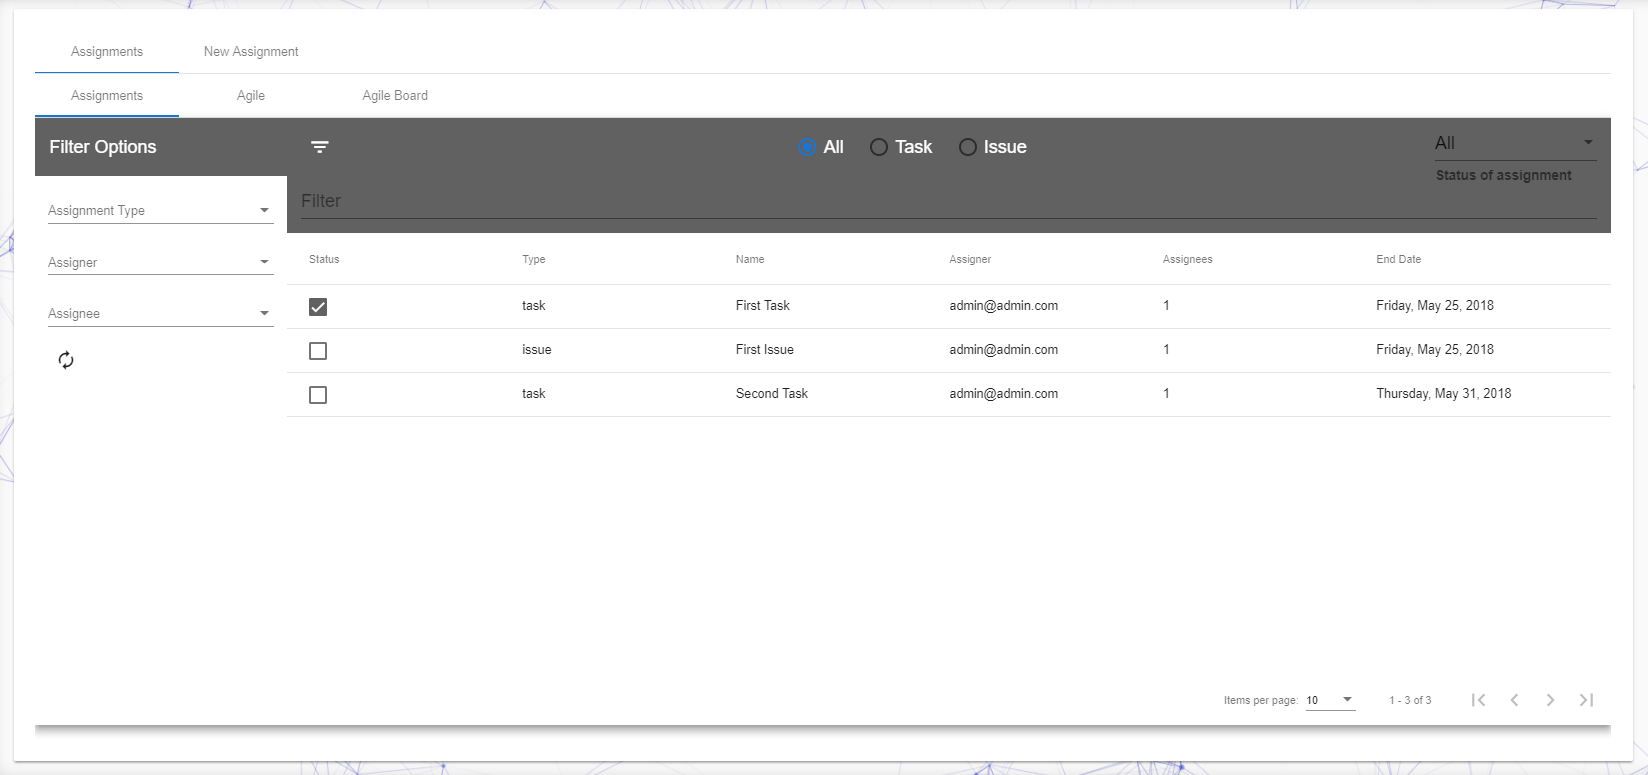
\includegraphics[width=\linewidth, height=8cm]{images/projectAssignments.png}
\caption{\e{Project - Assignments landing}}
\label{fig:projectAssignments}
\end{figure}

\pSpaceΌπως φαίνεται και απο το σχ. \ref{fig:projectAssignments}, υπάρχουν στον επάνω μέρος της καρτέλας δύο \e{tab}, \e{Assignments} και \e{New Assignment}.Θα εξηγήσουμε αρχικά το πρώτο.\\
\pSpaceΣτο πρώτο λοιπόν, περιλαμβάνονται άλλα τρία \e{tab} τα οποία φορτώνονται σε άλλη διεύθυνση σε σχέση με τα \e{tab} που υπήρχαν στην εφαρμογή.Το πρώτο στην σειρά αφορά μια κλασική απεικόνιση των εργασιών (βλ. σχ. \ref{fig:projectAssignmentsAssignments}), δηλαδή έναν πίνακα όπου η κάθε εγγραφή εκπροσωπεύει ένα \e{task} η \e{issue}.Η διεύθυνση αυτού είναι \e{\url{https://pmthesis.herokuapp.com/app/project/assignments/(assignments:assignments)}}.\\
\pSpaceΜια εγγραφή αποτελείται από την κατάσταση της εργασίας, ολοκληρωμενή η μή, ο τύπος (\e{Task, Issue}), τίτλος, ο χρήστης που την δημιούργησε, το σύνολο των μέλων στους οποίους αναθέτηκε αύτη η εργασία και η ημερομηνία στην οποία θα πρέπει να έχει ήδη ολοκληρωθεί.\\
\pSpaceΗ κατάσταση της εργασίας μπορεί να αλλάξει ενεργοποιώντας το \e{check box} που φαίνεται στην πρώτη στήλη, εφόσον ο χρήστης έχει πρόσβαση, δηλαδή να είναι δημιουργός η να ανήκει στην ομάδα των αναθετημένων.\\
\pSpaceΕπιλέγοντας μια εργασία, δηλαδή ενεργοποιώντας το κλίκ πάνω στην εγγραφή (εκτός \e{checkbox}), ανακατευθύνει τον χρήστη στην αναλυτική όψη.
\pSpaceΠάνω από τον πίνακα, παρατηρείται μια ομάδα από κουμπιά τύπου \e{radio}, ένα πεδίο \e{select} και ένα πεδίο κειμένου, τα οποία εκπληρώνουν την λειτουργία του φιλτραρίσματος.Τα φίλτρα που αναφέραμε, εφαρμόζονται ταυτοχρόνος, δηλαδή το αποτέλεσμα επηρεάζεται απο το σύνολο τους.\\
\pSpaceΕπιπλέον, στο αριστερό μέρος του πίνακα υπάρχει ένα μενού (επίσης με δυνατότητα απόκρυψης), στο οποίο βρίσκονται άλλα φίλτρα πιο συγκεκριμένα, προς το παρόν όμως δεν έιναι διαθέσιμα.\\
\pSpaceΟ πίνακας διαθέτει σελιδοποιήση και ρύθμιση των εγγραφών ανά σελίδα.

\begin{figure}[!htb]
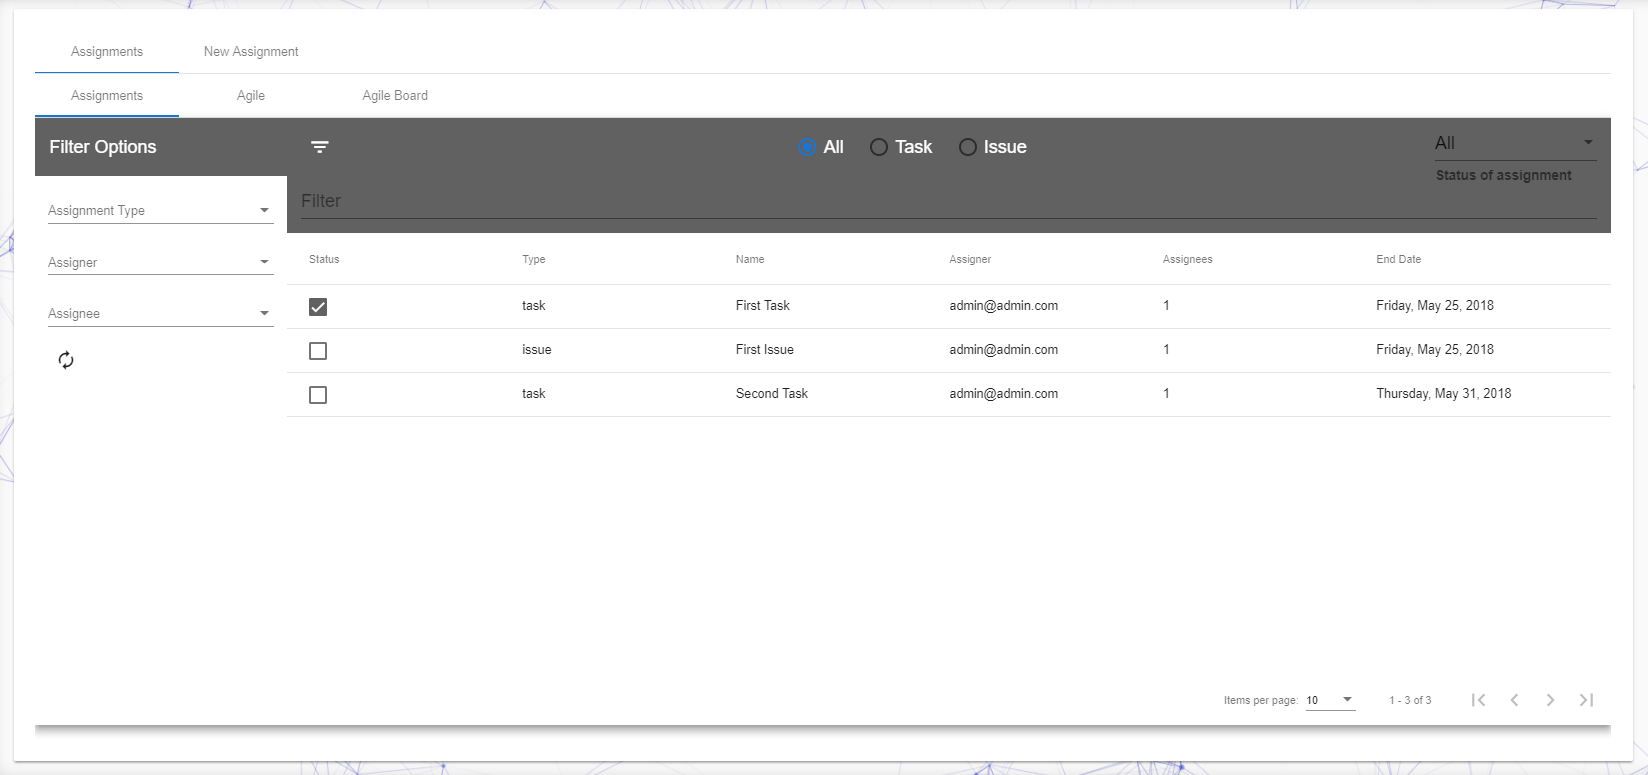
\includegraphics[width=\linewidth, height=8cm]{images/projectAssignmentsAssignments.png}
\caption{\e{Project - Assignments Classic}}
\label{fig:projectAssignmentsAssignments}
\end{figure}

\pSpaceΤα επόμενα δύο \e{tab}, δέν είναι διαθέσιμα προς το παρόν.\\

\pSpaceΤο \e{tab} με τίτλο \e{Create Assignment} (βλ. σχ. \ref{fig:projectCreateAssignment}) εξυπηρετεί την δημιουργία νέας εργασίας.Αποτελείται από τέσσερις \e{Expansion Panels} για να διευκολύνει την χρήση.Τα \e{panels} πηγαίνουν ως εξής:\\

\begin{itemize}
	\item Στο πρώτο εισάγονται τα βασικά στοιχεία όπως τύπος, τίτλος και μια σύντομη περιγραφή (2048 χαρακτήρες μέγιστο).
	\item Στο δεύτερο εισάγεται το εύρος ημερομηνιών.
	\item Το τρίτο αφορά τα άτομα στα οποία θα ανατεθεί η εν λόγω εργασία.Ο χρήστης μπορεί να πληκτρολογήσει τις ηλεκτρονικές διευθύνσεις η να επιλέξει από το αύτα που εμφανίζονται.Το συγκεκριμένο πεδίο είναι τύπου \e{select} αλλά και εισαγωγή κειμένου.Χωρίζοντας τις διευθύνσει με κόμμα, τις προσθέτει κατευθείαν στην λίστα.
	\item Το τελευταίο αφορά τις εξαρτήσεις.Αν επιλέξει να ορίσει κάποια η πολλαπλές εξαρτήσεις, θα ανοίξει ένα \e{modal} παράθυρο που περιέχει έναν πίνακα με τις υπαρκτές εργασίες και τον τύπο εξάρτησης.
\end{itemize}

\begin{figure}[!htb]
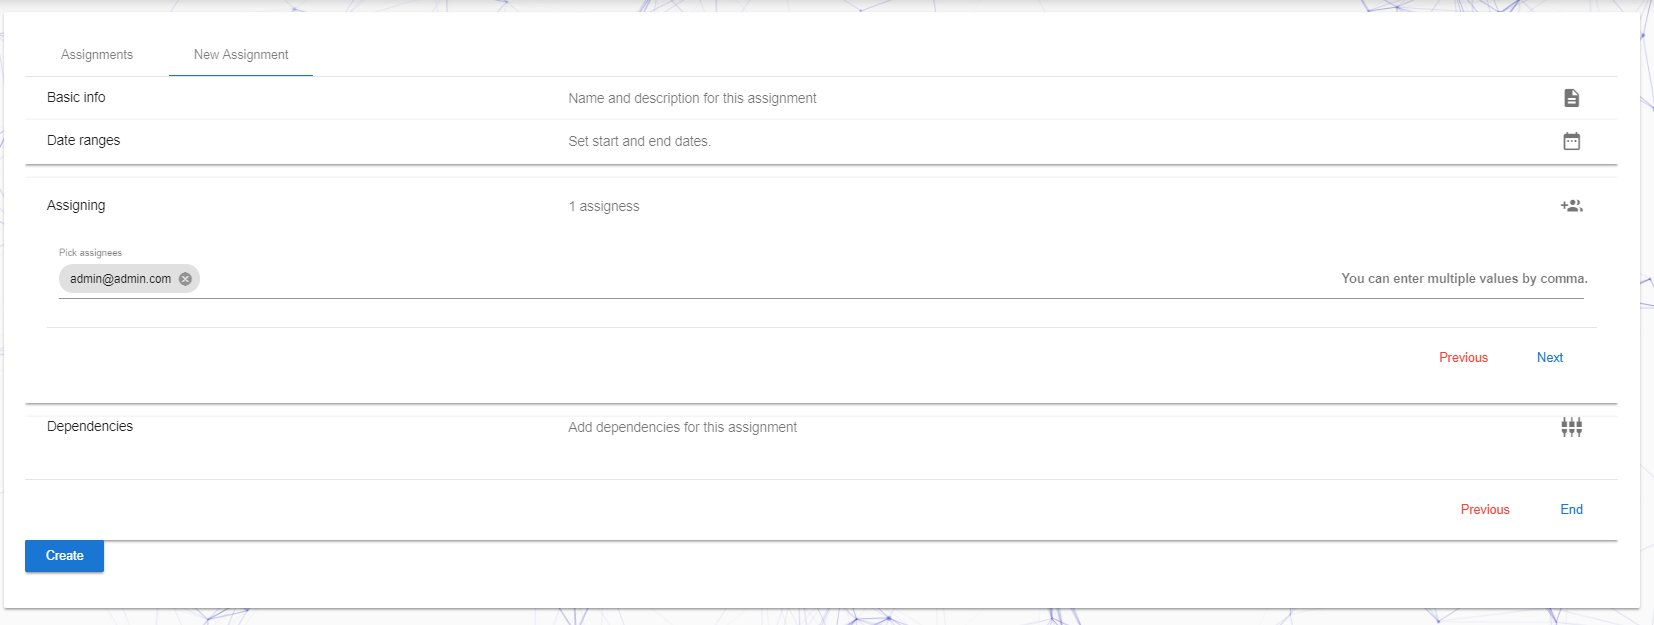
\includegraphics[width=\linewidth, height=8cm]{images/projectCreateAssignment.png}
\caption{\e{Project - Create Assignment}}
\label{fig:projectCreateAssignment}
\end{figure}

\pSpaceΕπιλέγοντας κάποια εργασία, ανακατευθύνει τον χρήστη στην διεύθυνση \e{\url{https://pmthesis.herokuapp.com/app/assignmentview/@id}} η οποία φορτώνει 2 καρτέλες, μια σχεδόν ίδια με το σχ. \ref{fig:projectCreateAssignment} και μια για τα σχόλια της έν λόγω εργασία.Η δεύτερη δεν είναι ακόμη διαθέσιμη.\\
\pSpaceΗ πρώτη καρτέλα έχει επιπλέον την κατάσταση της εργασίας ως διαφορές στο σχεδιασμό.Όμως, αν ο χρήστης επιθυμεί να την επεξεργαστεί, θα πρέπει να είναι είτε ο δημιουργός, είτε να ανήκει στην ομάδα των αναθετημένων, αλλίως όλα τα πεδία απενεργοποιούνται.

\begin{figure}[!htb]
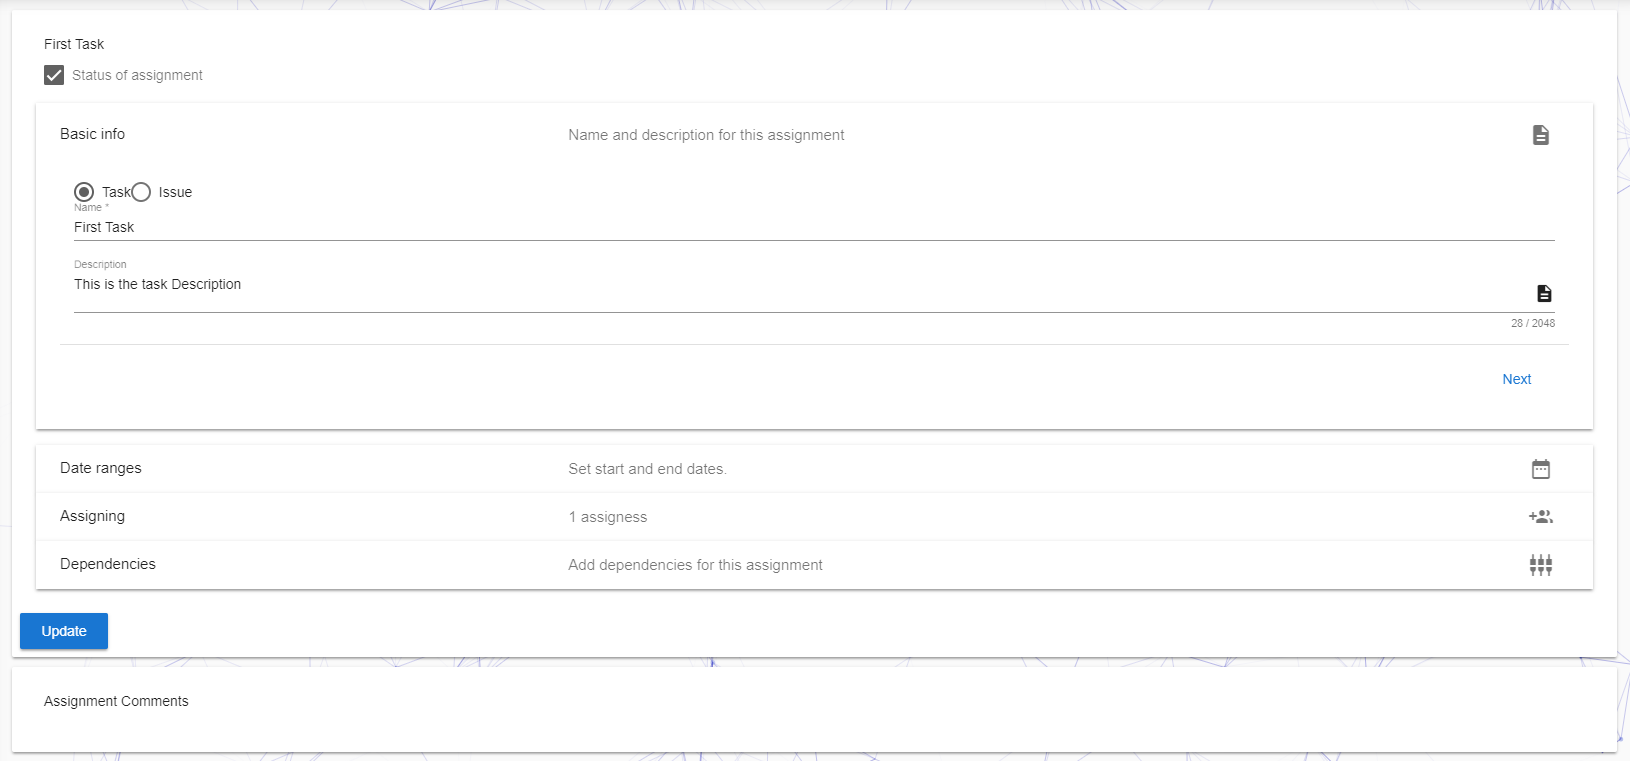
\includegraphics[width=\linewidth, height=8cm]{images/projectAssignementView.png}
\caption{\e{Project - Assignment View$\&$Edit}}
\label{fig:projectAssignmentView}
\end{figure}

\pagebreak

\subsubsection*{\e{Gantt}}
\pSpaceΗ διεύθυνση \e{\url{https://pmthesis.herokuapp.com/app/project/gantt}} φορτώνει την καρτέλα με το διάγραμμα Γκάνττ.Το διάγραμμα είναι ίδια με αυτήν που βρίσκεται στην ενότητα \e{User}, με την διαφορά ότι τα δεδομένα που προβάλλονται ανήκουν στο έργο και είναι μόνο τύπου \e{Task}.Οι εργασίες που έχουν κάποιου έιδους εξάρτηση μεταξύ τους είναι ομαδοποιημένα, και σχετίζονται με βελάκια που παριστάνουν την εξάρτηση.

\begin{figure}[!htb]
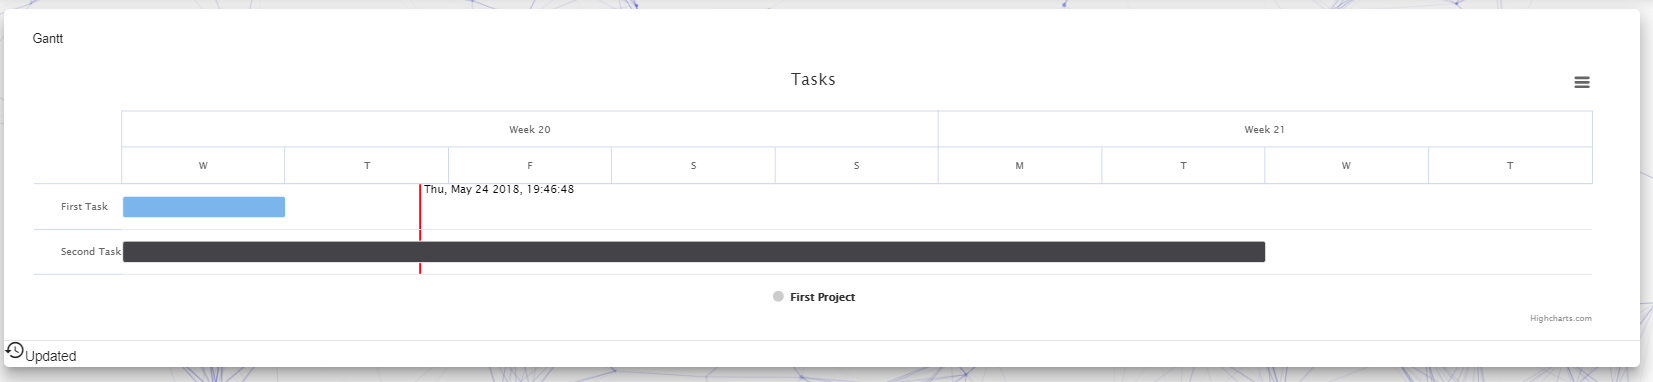
\includegraphics[width=\linewidth, height=6cm]{images/projectGantt.png}
\caption{\e{Project - Gantt}}
\label{fig:projectGantt}
\end{figure}

\subsubsection*{\e{Team}}
\pSpaceΗ επόμενη επιλογή στο αριστερό μενού, στην ενότητα έργου, είναι το \e{Team}, με διεύθυνση \e{\url{https://pmthesis.herokuapp.com/app/project/team}}.Φορτώνει στο πλαίσιο δεδομένων δύο καρτέλες (βλ. σχ. \ref{fig:projectTeam}).\\
\pSpaceΣτην πρώτη καρτέλα, απεικονίζεται η ομάδα του έργου σε μορφή πίνακας, κάθε εγγραφή παριστάνωντας ένα μέλο με τις ακόλουθες πληροφορίες: αριθμός, ηλεκτρονική διεύθυνση, ρόλο.Σε κάθε εγγραφή, δίνεται η δυνατότητα αφαίρεσης της, και έμμεσα του μέλους από την ομάδα.\\
\pSpaceΣτην δεύτερη καρτέλα υπάρχει ένα πεδίο κειμένου, όπως αυτό στην δημιουργία έργου, όπου πληκτρολογεί ο χρήστης τα άτομα που επιθυμεί να προσκαλέσει στην ομάδα.

\begin{figure}[!htb]
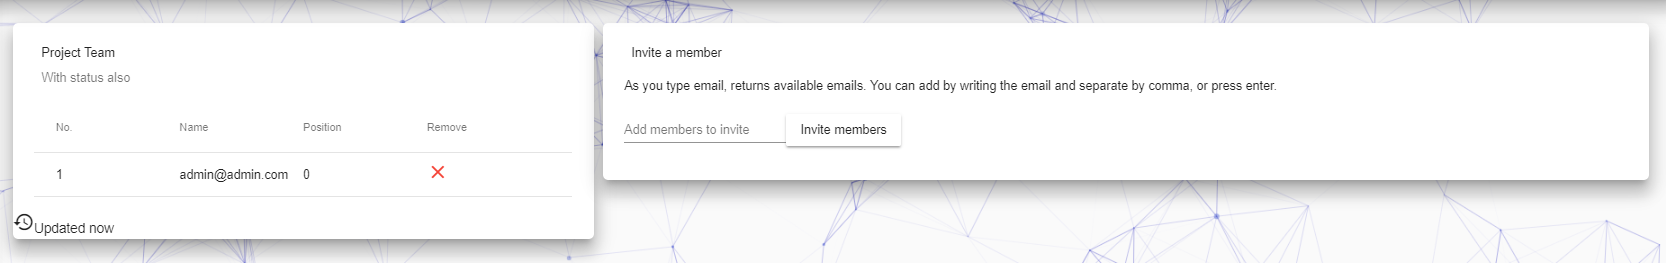
\includegraphics[width=\linewidth]{images/projectTeam.png}
\caption{\e{Project - Team}}
\label{fig:projectTeam}
\end{figure}

\subsubsection*{\e{Action Log}}
\pSpaceΤο \e{Action Log} αναφέρεται στο χρονοδιάγραμμα έργου, όπου σημειώνονται τα σημαντικότερα σύμβαντα.Βρίσκεται στην διεύθυνση \e{\url{https://pmthesis.herokuapp.com/app/project/timeline}} και φορτώνει την καρτέλα του σχ. \ref{fig:projectTimeline}.\\
\pSpaceΗ σειρά των εγγραφών είναι με βάση τις ημερομηνίες τους.Επιλέγοντας κάποια εγγραφή του χρονοδιαγράμματος, εμφανίζει κάτω από τον ίδιο περαιτέρω πληροφορίες σχετικά με αυτήν.

\begin{figure}[!htb]
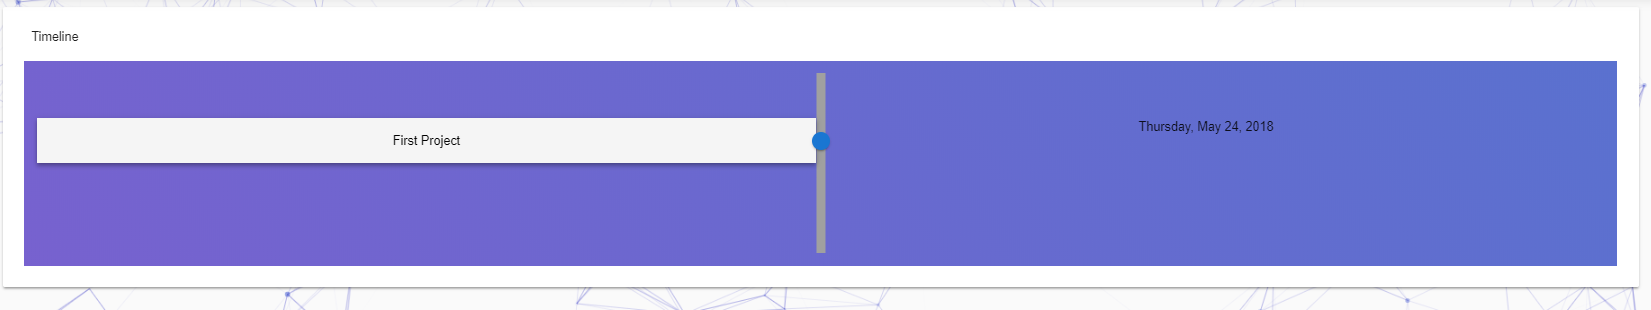
\includegraphics[width=\linewidth]{images/projectTimeline.png}
\caption{\e{Project - Action Log}}
\label{fig:projectTimeline}
\end{figure}

\subsubsection*{\e{Settings}}
\pSpaceΤελευταία επιλογή του μενού, πηγαίνει τον χρήστη στις ρυθμίσεις έργου, οι οποίες έιναι προσβάσιμες άν ο χρήστης έιναι ο διαχειριστής, αλλίως τον ανακατευθύνει στο \e{Dashboard} έργου.Η διεύθυνση \e{\url{https://pmthesis.herokuapp.com/app/project/settings}} φορτώνει στον πλαίσιο δεδομένων δύο καρτέλες (βλ. σχ. \ref{fig:projectSettings}).Και οι δύο αποτελούνται από τέσσερα \e{Expansion Panels}.\\
\pSpaceΗ πρώτη καρτέλα, αφορά τα βασικά στοιχεία του έργου τα οποία εισάχθηκαν στην δημιουργία:\\
\begin{itemize}
	\item Εταιρία
	\item Τίτλος
	\item Προυπολογισμός
	\item Σύντομη περιγραφή
\end{itemize}

\pSpaceΗ δεύτερη καρτέλα αφορά ρυθμίσεις που χρειάζονται όλη την προσοχή του διαχειριστή:\\

\begin{itemize}
	\item \e{Privacy} - Αν το έργο είναι ιδιωτικό η δημόσιο.Αυτό επηρεάζει τα αποτελέσματα αναζήτησης.
	\item Ιδιοκτησία - Εδώ ο διαχειριστής, μπορεί να δώσει τον ρόλο του σε άλλο μέλος του έργου.
	\item Κλείδωση - Αν αποφασίσει να κλειδώσει το έργο ο διαχειριστής, σημαίνει πώς δεν μπορούν να λάβουν θέση άλλες ενέργειες, παρά μόνο προβολή των πληροφοριών.
	\item Διαγραφή - Διαγραφή έργου και όλως των δεδομένων (\e{Task, Issue} κλπ)
\end{itemize}

\pSpaceΤο κουμπί στο δεξιό μέρος του πλαισίου δεδομένων έχει τον ρόλο αποθήκευσης αλλαγών.

\begin{figure}[!htb]
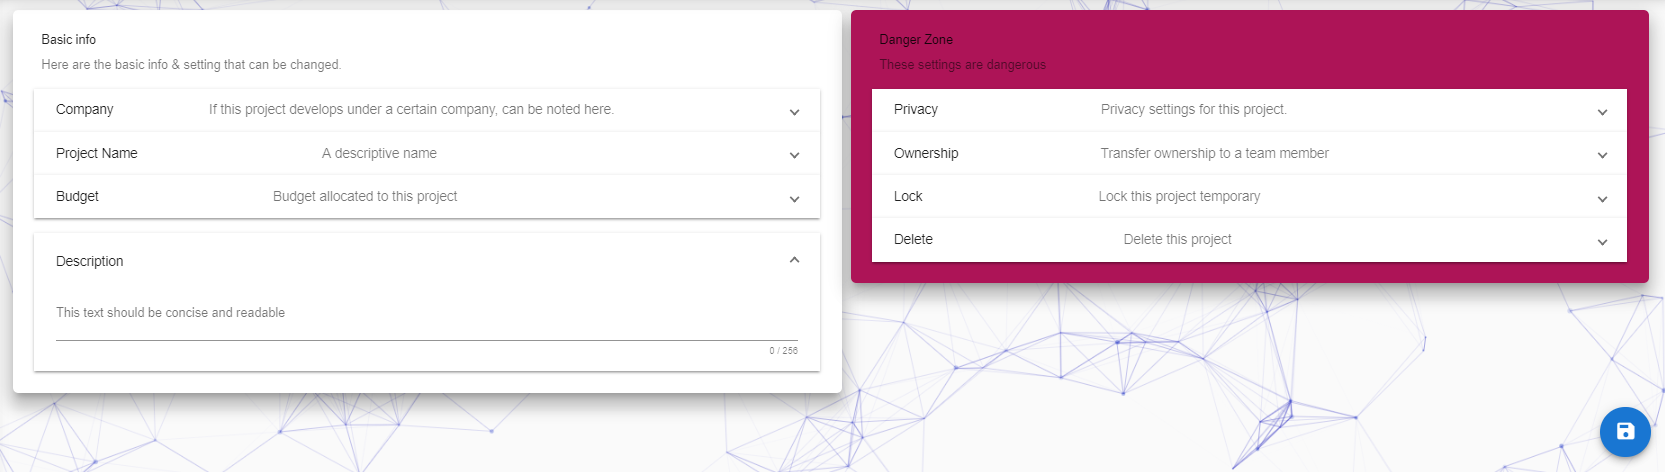
\includegraphics[width=\linewidth]{images/projectSettings.png}
\caption{\e{Project - Settings}}
\label{fig:projectSettings}
\end{figure}

\subsubsection*{\e{Notifications}}
\pSpaceΟι ειδοποιήσεις είναι τύπου \e{Push} (βλ. σχ. \ref{fig:pushNotification}), και χρειάζονται την αποδοχή του χρήστη για να εμφανιστούν.Περιέχουν τίτλο, περιγραφή και σε μερικές περιπτώσεις συνδέσμους για γρήγορα πρόσβαση στις υπόλοιπες πληροφορίες.\\
\pSpaceΕπιπλέον, το σύνολο ειδοποιήσεων φαίνονται ενεργοποιώντας τον διακόπτη για το δεξιό μενού, απο την πάνω γραμμή εργαλειών.Αυτό ανοίγει τα \e{Notifications} ομαδοποιημένα σε δύο κατηγορίες: \e{Seen, Unseen} (βλ. σχ. \ref{fig:userNotifications}).

\begin{figure}[!htb]
\centering

\includegraphics[scale=0.5]{images/pushNotification.png}
\caption{\e{Notification}}
\label{fig:pushNotification}
\end{figure}

\begin{figure}[!htb]
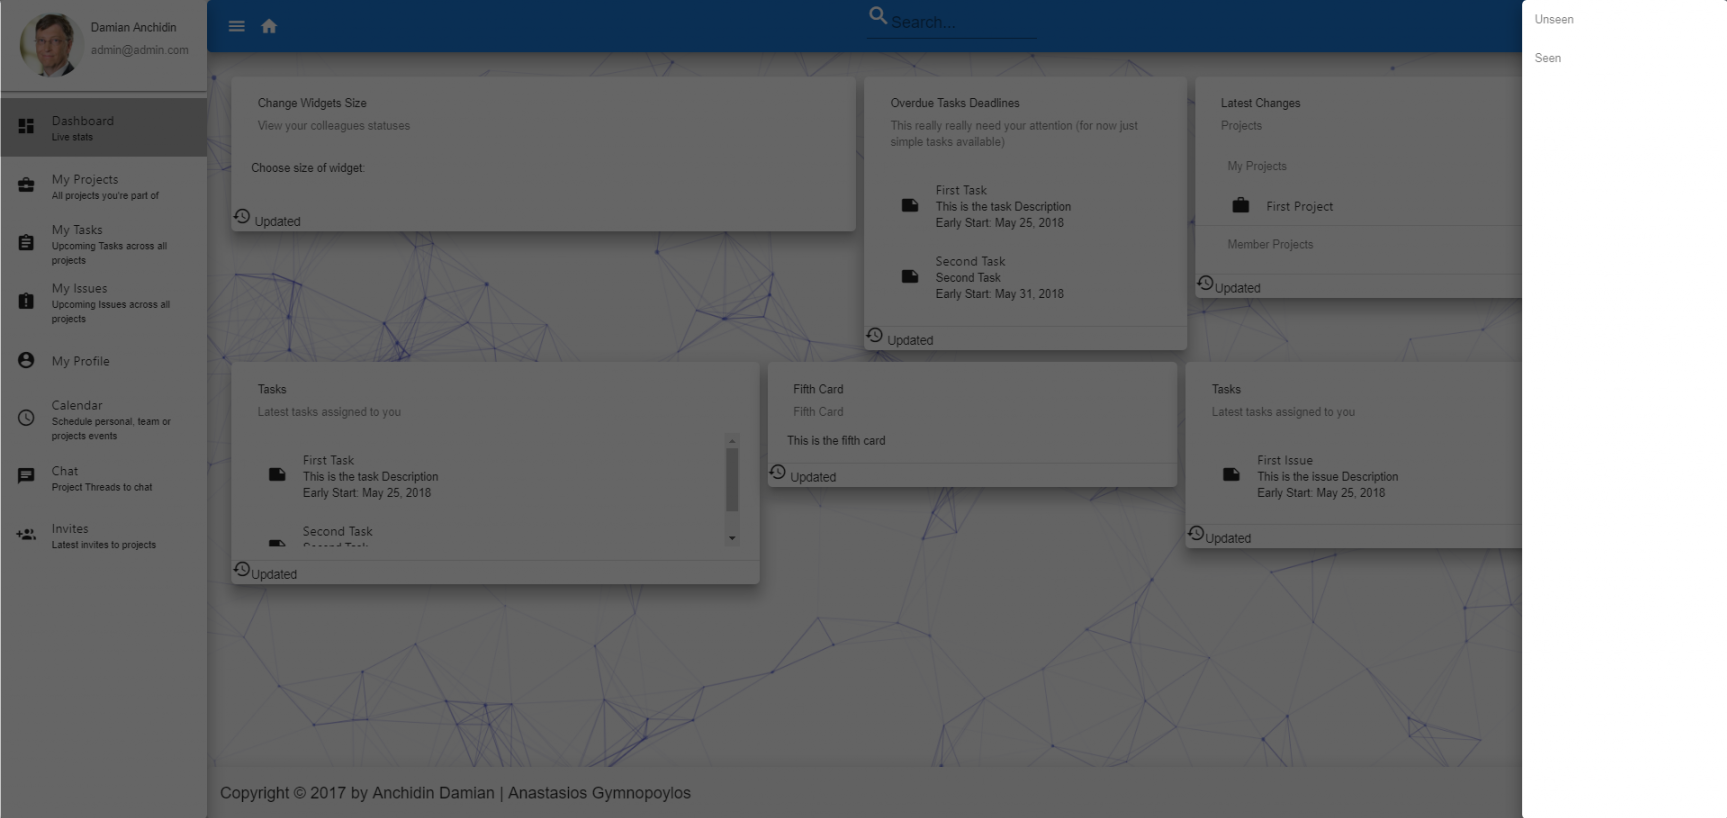
\includegraphics[width=\linewidth]{images/userNotifications.png}
\caption{\e{Notifications}}
\label{fig:userNotifications}
\end{figure}

\subsubsection*{\e{Theme}}
\pSpaceΤο κουμπί για το θέμα σχεδιασμού που βρίσκεται στην πάνω γραμμή εργαλειών, ανοίγει ένα \e{Context Menu} με τέσσερις επιλογές (δύο διαθέσιμες).Η μια είναι η προκαθορισμένη, ενώ η δεύτερη φαίνεται στο σχ. \ref{fig:userDashboardDark}.

\begin{figure}[!htb]
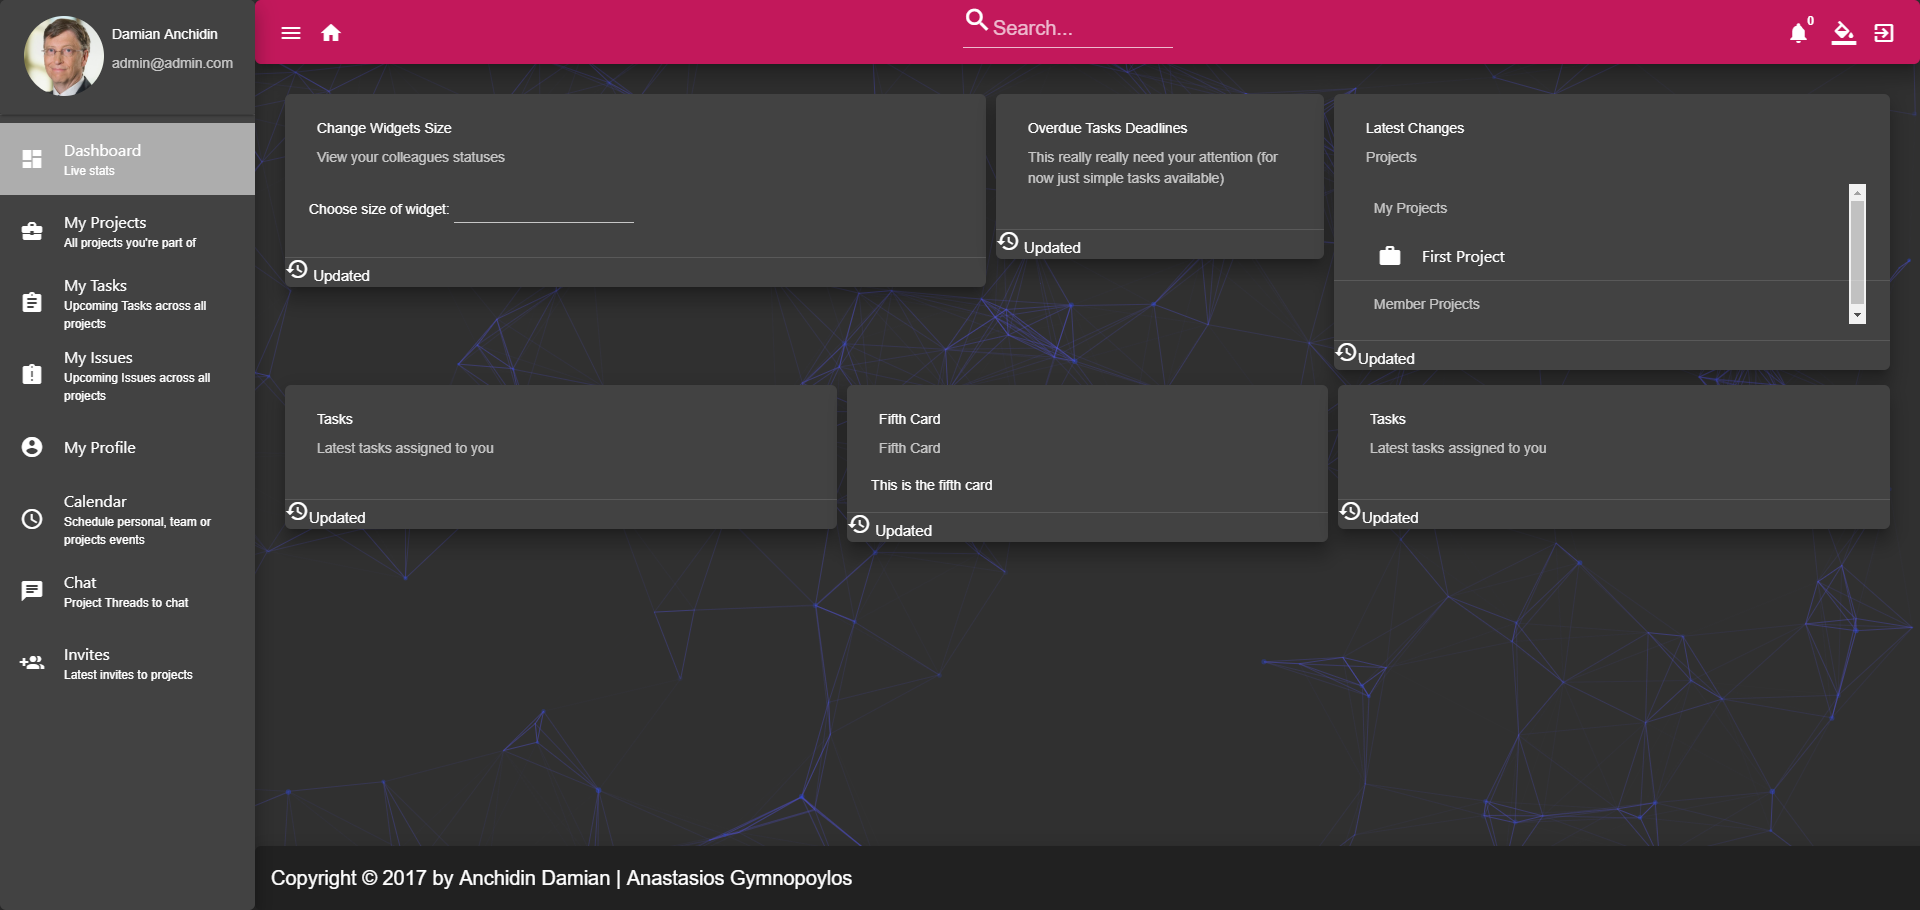
\includegraphics[width=\linewidth]{images/userDashboardTHEME2.png}
\caption{\e{Dark Theme}}
\label{fig:userDashboardDark}
\end{figure}

% /Project actions

\chapter{Συμπεράσματα}
\subsection*{Συμπεράσματα}
\pSpace Οι εφαρμογές και το διαδίκτυο αποτελούν σήμερα τα απαραίτητα εργαλεία στην διαχείριση έργων. Καθώς η τεχνολογία προχωράει και οι θεωρίες πολλαλασιάζονται περί του θέματος, οι χρήστες ψάχνουν την καλύτερη δυνατή λύση. Όμως, ο συνδυασμός των βασικών αναγκών, η εύκολη χρήση και η εξοικονόμηση χρόνου οδηγεί τους δημιουργούς να ψάχνουν ανάμεσα απο τις καλύτερες λύσεις, που προσφέρονται στην αγορά, μια λύση που να εκπληρώνει τον συνδυασμό αυτό.\\
\pSpace Στην αρχή της παρούσας εργασίας ο σκοπός που τέθηκε ήταν η κατασκεύη μια διαδικτυακής εφαρμογής για την διαχείριση έργων, που στοχεύει την απλότητα και εύκολη χρήση της.\\
\pSpace Ύστερα από κάποιες δοκιμές απο άτομα με διαφορετικό επίπεδο γνώσεων ως πρός το \e{Project Management}, φτάσαμε στο συμπεράσμα πως η εφαρμογή έχει εκπληρώσει τον σκοπό της. Ενώ στερεί σε αριθμό λειτουργιών, παρατηρήθηκε πως ο χρήστης ήταν ικανοποιημένος κυρίως από την απλή χρήση και την εξοικονόμηση χρόνου. Όπως ήταν αναμενόμενο, στις περιπτώσεις όπου τα έργα ήταν μεγαλύτερου μεγέθους, απαιτείται μια λύση που να καλύπτει περισσότερες λειτουργίες.\\
\pSpace Ένας δεύτερος σκοπός που έχει τεθεί, ως προς την υλοποίηση, ήταν ο σωστός συνδυασμός των δύο γνωστών πρότυπων προγραμματισμού, Αντικειμενοστραφής και Αντιδραστικός.\\
\pSpace Το δυσκολότερο κομμάτι για την επίτευξη αυτού του σκοπού, ήταν η συνήθεια στην Αντιδραστική σκέψη. Χρησιμοποιώντας αύτο το πρότυπο, άλλες πρακτικές του προγραμματισμού έπρεπε να απορριφθούν καθώς ήταν ανούσιες η έκαναν τον κώδικα πολύπλοκο χωρίς κάποιο κέρδος.\\
\pSpace Φτάσαμε στο συμπεράσμα όμως, ότι ο συνδυασμός των δύο δεν συνιστάται αν οι προγραμματιστές δεν αποφασίσουν ομαδικά να ακολουθούν ένα αντιδραστικό τρόπο ανάπτυξης. Επίσης, η επίτευξη αυτού του σκοπού θεωρήθηκε ομαδικώς, ότι έχει ολοκληρωθεί κατά 85 $\%$.\\

\subsection*{Επεκτασιμότητα και βελτιώσεις}
\pSpace Η εφαρμογή βρίσκεται αύτην την στιγμή σε ένα πολύ βασικό στάδιο, αλλά μπορεί να αναπτυχθεί σε αρκετά υψηλότερο επίπεδο κρατώντας την ίδια βάση.\\
\pSpace Μια επέκταση αυτής της εφαρμογής είναι να προστεθεί η δυνατότητα προβολής \e{Agile} των εργασιών. Παρόλο, που αυτή η λειτουργία ήταν διαθέσιμη, δεν αποτελούσε μια πρακτική λύση στην μορφή που βρισκόταν.\\
\pSpace Μια άλλη ιδέα επέκτασης είναι η ενσωμάτωση διάφορων γνωστών εργαλείων, όπως \e{Dropbox, GoogleDrive, Slack} η \e{Github}.\\
\pSpace Η εφαρμογή μπορεί να βελτιωθεί ξεκινώντας από τις υπηρεσίες ειδοποιήσεων και προσκλήσεων, έτσι ώστε η εμπειρία του χρήστη να βελτιωθεί. Προς το παρόν οι δύο αναφερόμενες υπηρεσίες στερούν στό επίπεδο χρησιμότητας που επιθυμείται. Το ίδιο ισχύει για την εφαρμογή σε κινητό περιβάλλον, όπου ίσως ο σχεδιασμός να είναι το μεγαλύτερο πρόβλημα.


\addcontentsline{toc}{chapter}{\textgreek{Βιβλιογραφία}}
\selectlanguage{english}
\printbibliography
\end{document}
